% Escolha: Portugues ou Ingles ou Espanhol.
% Para a versão final do texto, após a defesa acrescente Final:


\documentclass[Ingles,Final]{ic-tese-v3}
% \documentclass[Portugues,Final]{ic-tese-v3}

\usepackage[latin1,utf8]{inputenc}
\usepackage{babel} 
%\usepackage{pdflscape}
\usepackage{rotating}
\usepackage{tikz}
\usepackage{xcolor}
\usepackage{enumitem}
\usepackage {subfig}
\usepackage {float}
% Para acrescentar comentários ao PDF descomente:
% \usepackage
%  [pdfauthor={Augusto F. R. Queiroz},
%   pdftitle={Secure code execution using PUF authentication},
%   pdfkeywords={PUF}]%,
% %   pdfproducer={Latex with hyperref},
% %   pdfcreator={pdflatex}]
% {hyperref}
\usepackage{hyperref}


% *** GRAPHICS RELATED PACKAGES ***w

\usepackage{graphicx,url, float}
%    \ifCLASSINFOpdf
%        \usepackage[pdftex]{graphicx,url}
        \graphicspath{{figures/pdf/}}
        \DeclareGraphicsExtensions{.pdf}
%    \else
%        \usepackage[dvips]{graphicx,url}
%        \graphicspath{{figures_eps/}}
%        \DeclareGraphicsExtensions{.eps}
%    \fi

% *** MATH PACKAGES ***
\usepackage{amssymb}  

% *** ALGORITHM PACKAGES ***
\usepackage{algorithm}
\usepackage{algorithmic}

% *** CITATION PACKAGE ***
\usepackage{cite}

% *** MISC UTILITY PACKAGES ***
% \usepackage{ulem}
\usepackage{multirow}
\usepackage[printonlyused]{acronym}

% *** COMMANDS ***
\newcommand{\cald}{{\cal D}}
\newcommand{\calh}{{\cal H}}
\newcommand{\calj}{{\cal J}}
\newcommand{\calm}{{\cal M}}
\newcommand{\caln}{{\cal N}}
\newcommand{\cals}{{\cal S}}
\newcommand{\calt}{{\cal T}}
\newcommand{\calv}{{\cal V}}

\begin{document}

% Escolha entre autor ou autora:
\autor{Augusto Fernandes Ribas Queiroz }


% Sempre deve haver um título em português:
\titulo{Execução segura de códigos utilizando PUF para autenticação}

% Se a língua for o inglês ou o espanhol defina:
\title{Secure code execution using PUF authentication}

% Escolha entre orientador ou orientadora. Inclua os títulos acadêmicos:
\orientador{Prof. Dr.Guido Costa Souza de Araújo}
%\orientadora{Profa. Dra. Nome da Orientadora}

% Escolha entre coorientador ou coorientadora, se houver.  Inclua os títulos acadêmicos:
\coorientador{Prof. Dr.Mário Lúcio Côrtes}


% Escolha entre mestrado ou doutorado:
\mestrado
%\doutorado

% Se houve cotutela, defina:
%\cotutela{Universidade Nova de Plutão}

\datadadefesa{28}{03}{2019}

% Para a versão final defina:
\avaliadorA{Prof. Dr. someone}{Universidade Estadual de Campinas}
\avaliadorB{Prof. Dr.Someonel}{Universidade Federal de Santa Catarina}
\avaliadorC{Profa. Dra. someone}{Universidade Estadual de Campinas}


% Para incluir a ficha catalográfica em PDF na versão final, descomente e ajuste:
%\fichacatalografica{includes/Ficha-Catalografica-Protocolo-325698704.pdf}



% Definitions
\def\socs{SoCs}
\def\prf{PRF}
\def\prfs{PRFs}
\def\sram{SRAM}
\def\srams{SRAMs}
\def\spuf{SPUF}
\def\spufs{SPUFs}
\def\tagsystem{SEC-ENG}
\def\mctrl{MCTRL}
\def\system{CSHIA}
\def\seccache{SEC-CACHE}
\def\thetitle{Secure code execution using PUF authentication}



% Definitions
\def\phd{Ph.D.}
\def\iot{IoT}
\def\iots{IoTs}
\def\soc{SoC}
\def\cpu{CPU}
\def\socs{SoCs}
\def\asic{ASIC}
\def\asics{ASICs}
\def\puf{PUF}
\def\pufs{PUFs}
\def\prp{PRP}
\def\prps{PRPs}
\def\prf{PRF}
\def\prfs{PRFs}
\def\sram{SRAM}
\def\srams{SRAMs}
\def\spuf{SPUF}
\def\spufs{SPUFs}
\def\seceng{SEC-ENG}
\def\mctrl{MCTRL}
\def\pmmu{PMMU}
\def\handler{BUS-HDLR}
\def\cshia{CSHIA}
\def\fuzzy{Fuzzy Extractor}
\def\fe{FE}
\def\fes{FEs}
\def\ptag{PTAG}
\def\ptags{PTAGs}
\def\pufarch{PUF Architecture}
\def\pufarchs{PUF Architectures}
\def\puf{PUF}
\def\apuf{APUF}
\def\pufs{PUFs}
\def\apufs{APUFs}
%\def\icache{ICL}
%\def\icaches{ICLs}
%\def\dcache{DCL}
%\def\dcaches{DCLs}
\def\icache{LIC}
\def\icaches{LICs}
\def\dcache{LDC}
\def\dcaches{LDCs}
\def\ptaggen{PTAG-GEN}
\def\ptagnmi{PTAG-NMI}
\def\ptagmem{PTAG Memory}
\def\ptagcache{PTAG Cache}
\def\fpga{FPGA}
\def\fpgas{FPGAs}
\def\vhdl{VHDL}
\def\siphash{SipHash}
\def\nopolicy{Caching.Path}
\def\chtree{CHTree}
\def\readhit{Read.Hit}
\def\secbus{SecBus}
\def\etal{\textit{et al.}}
\def\mt{Merkle Tree}
\def\voting{TMV}
\def\bch{BCH}
\def\ibs{IBS}
\def\ecc{ECC}
\def\isa{ISA}
\def\aes{AES}
\def\lru{LRU}
\def\alap{ALAP}
\def\leon{Leon3}
\def\amba{AMBA}
\def\dsu{DSU}
\def\grmon{GRMON}
\def\cacti{CACTI}
\def\epe{EPE}
\def\baseline{\textit{Leon3 Baseline}}
\def\timestamp{\textit{\cshia-TS}}
\def\cshiamt{\textit{\cshia-MT}}
\def\attacker{he\slash{}she}
\def\Attacker{he\slash{}she}
\def\hisher{his\slash{}her}
\def\Hisher{His\slash{}her}
\def\crp{CRP}
\def\crps{CRPs}
\def\andor{and\slash{}or}
\def\xom{XOM}
\def\aegis{AEGIS}
\def\fedtic{FEDTIC}
\def\lone{L1}
\def\ltwo{L2}
\def\lut{LUT}
\def\luts{LUTs}
\def\otp{OTP}
\def\crc{CRC}
\def\io{I\slash{}O}
\def\ios{I\slash{}Os}
\def\amba{AMBA2}
\def\sline{SEC Line}
\def\slines{SEC Lines}
\def\sbuf{BHS Buffer}
% To turn comments OFF simply comment out the \Commentstrue line
\newif\ifComments
\Commentstrue

\ifComments
\newcommand{\chek}[1]{\textcolor{red}{Check: {#1}}}
\newcommand{\liana}[1]{\textcolor{purple}{Liana: {#1}}}
\newcommand{\gabi}[1]{\textcolor{purple}{Gabi: {#1}}}
\newcommand{\augusto}[1]{\textcolor{violet}{Augusto: {#1}}}
\newcommand{\guido}[1]{\textcolor{magenta}{Guido: {#1}}}
\newcommand{\mario}[1]{\textcolor{olive}{Mario: {#1}}}
\newcommand{\rem}[1]{\textcolor{gray}{\sout{#1}}}
\newcommand{\new}[1]{\textcolor{blue}{ {#1}}}
\newcommand{\ed}[1]{\textcolor{red}{ {#1}}}
\newcommand{\short}[1]{\textcolor{blue}{ {#1}}}
\else
\newcommand{\augusto}[1]{}
\newcommand{\liana}[1]{}
\newcommand{\gabi}[1]{}
\newcommand{\chek}[1]{}
\newcommand{\caio}[1]{}
\newcommand{\guido}[1]{}
\newcommand{\mario}[1]{}
\newcommand{\rem}[1]{}
\newcommand{\new}[1]{#1}
\newcommand{\ed}[1]{#1}
\newcommand{\short}[1]{}
\fi

% Este comando deve ficar aqui:
\paginasiniciais


\prefacesection{Dedicatória}
Lorem ipsum dolor sit amet, consectetur adipiscing elit. Phasellus vitae iaculis erat. Aliquam tristique consectetur ante, quis commodo lacus egestas in. Nullam semper elit nec eros pretium 


% Se houver epígrafe, descomente e edite:
% \begin{epigrafe}
% {\it
% Vita brevis,\\
% ars longa,\\
% occasio praeceps,\\
% experimentum periculosum,\\
% iudicium difficile.}
%
% \hfill (Hippocrates)
% \end{epigrafe}


% Agradecimentos ou Acknowledgements ou Agradecimientos
% \prefacesection{Agradecimentos}
% Os agradecimentos devem ocupar uma única página.


% Sempre deve haver um resumo em português:
\begin{resumo}
Lorem ipsum dolor sit amet, consectetur adipiscing elit. Phasellus vitae iaculis erat. Aliquam tristique consectetur ante, quis commodo lacus egestas in. Nullam semper elit nec eros pretium dapibus. Ut eget porta metus. Mauris rhoncus vel magna non faucibus. Ut a ornare elit. Morbi sagittis quam nec risus laoreet, tincidunt volutpat ex venenatis. Sed ultrices felis quis felis scelerisque gravida a non neque. Etiam sed nisi neque. Ut lobortis pulvinar facilisis. Vestibulum quis enim bibendum, iaculis nulla non, consequat nunc. Suspendisse sed hendrerit tortor, non maximus lorem. Ut sit amet turpis eget libero condimentum scelerisque. Quisque sed dolor metus.

Cras ac tincidunt tellus. Morbi id interdum magna, a ornare justo. Praesent tincidunt tempus porta. Sed iaculis fermentum nibh non porta. Aenean mattis sapien purus, ut ornare risus ornare non. Integer sit amet neque auctor, interdum mi in, sodales sem. Pellentesque at rutrum quam, eget posuere elit. Donec nec tortor egestas, laoreet ligula sit amet, luctus felis. Proin sit amet tempor odio. Sed orci orci, gravida dignissim molestie id, fringilla nec ligula.

Aenean pharetra, massa eu dapibus malesuada, lacus nisl auctor magna, in tempor nulla ante et ante. Mauris in purus lacus. Nam ac enim et ipsum condimentum vehicula. Mauris pulvinar facilisis lacus, non ultrices risus tempus a. Lorem ipsum dolor sit amet, consectetur adipiscing elit. Donec auctor sagittis lacinia. Fusce porta dapibus vulputate.

Nam posuere lacus nulla, nec pharetra nisi tempor vitae. Sed ac erat eget lacus ultrices tincidunt. Aliquam egestas quam vitae magna semper tempor. Nam at diam sit amet eros bibendum efficitur at ac neque. Morbi rhoncus ullamcorper erat, porta rutrum lacus tincidunt non. Nunc eget tellus eu nulla ornare ullamcorper et sit amet nulla. Vivamus in erat ultrices, faucibus velit sit amet, feugiat massa. Ut lacinia mattis quam ac posuere. Praesent et eros mauris. Nullam malesuada mauris diam, sed varius tortor posuere at. Aenean volutpat suscipit tortor vel blandit. Nullam euismod est a suscipit tempus.
\end{resumo}


% Sempre deve haver um abstract:
\begin{abstract}
% The abstract must have at most 500 words and must fit in a single page.

Lorem ipsum dolor sit amet, consectetur adipiscing elit. Phasellus vitae iaculis erat. Aliquam tristique consectetur ante, quis commodo lacus egestas in. Nullam semper elit nec eros pretium dapibus. Ut eget porta metus. Mauris rhoncus vel magna non faucibus. Ut a ornare elit. Morbi sagittis quam nec risus laoreet, tincidunt volutpat ex venenatis. Sed ultrices felis quis felis scelerisque gravida a non neque. Etiam sed nisi neque. Ut lobortis pulvinar facilisis. Vestibulum quis enim bibendum, iaculis nulla non, consequat nunc. Suspendisse sed hendrerit tortor, non maximus lorem. Ut sit amet turpis eget libero condimentum scelerisque. Quisque sed dolor metus.

Cras ac tincidunt tellus. Morbi id interdum magna, a ornare justo. Praesent tincidunt tempus porta. Sed iaculis fermentum nibh non porta. Aenean mattis sapien purus, ut ornare risus ornare non. Integer sit amet neque auctor, interdum mi in, sodales sem. Pellentesque at rutrum quam, eget posuere elit. Donec nec tortor egestas, laoreet ligula sit amet, luctus felis. Proin sit amet tempor odio. Sed orci orci, gravida dignissim molestie id, fringilla nec ligula.

Aenean pharetra, massa eu dapibus malesuada, lacus nisl auctor magna, in tempor nulla ante et ante. Mauris in purus lacus. Nam ac enim et ipsum condimentum vehicula. Mauris pulvinar facilisis lacus, non ultrices risus tempus a. Lorem ipsum dolor sit amet, consectetur adipiscing elit. Donec auctor sagittis lacinia. Fusce porta dapibus vulputate.

Nam posuere lacus nulla, nec pharetra nisi tempor vitae. Sed ac erat eget lacus ultrices tincidunt. Aliquam egestas quam vitae magna semper tempor. Nam at diam sit amet eros bibendum efficitur at ac neque. Morbi rhoncus ullamcorper erat, porta rutrum lacus tincidunt non. Nunc eget tellus eu nulla ornare ullamcorper et sit amet nulla. Vivamus in erat ultrices, faucibus velit sit amet, feugiat massa. Ut lacinia mattis quam ac posuere. Praesent et eros mauris. Nullam malesuada mauris diam, sed varius tortor posuere at. Aenean volutpat suscipit tortor vel blandit. Nullam euismod est a suscipit tempus.

\end{abstract}




% A lista de figuras é opcional:
\listoffigures

% A lista de tabelas é opcional:
\listoftables

% A lista de abreviações e siglas é opcional:
% \prefacesection{Lista de Abreviações e Siglas}

% A lista de símbolos é opcional:
% \prefacesection{Lista de Símbolos}

% Quem usa o pacote nomencl pode incluir:
%\renewcommand{\nomname}{Lista de Abreviações e Siglas}
%\printnomenclature[3cm]


% O sumário vem aqui:
\tableofcontents


% E esta linha deve ficar bem aqui:
\fimdaspaginasiniciais


% O corpo da dissertação ou tese começa aqui:
%this  group is to remove the spaces afte the chapters 
%\begingroup 
% this is a ugly hack to clear the inserted clearpages - this is messing with the references!
% \renewcommand{\cleardoublepage}{}
% \renewcommand{\clearpage}{}

\chapter{Introduction}
\label{chap:introduction}

%TODO USE BOTH SOC AND EMBEDDED?
%SOC
%Standard design techniques to secure code execution in \socs~are based on well-known cryptographic mechanisms and on (micro) architecture features to encode bus transactions~\cite{Elbaz2005}, or isolate secure code into trusted platforms~\cite{tpm_spec}, among others. Although such techniques usually provide good levels of security, most of them are either inefficient, considerably impact processor (micro) architecture design, require extensive changes in the programming tool-chain~\cite{Suh2003a}, or are so complex \cite{Suh2005} that may create unexpected security loopholes. Any solution up to this challenge should be able to use more than incremental approaches which try to re-use current cryptographic mechanisms to fill in security holes; the new generation of \iot~\soc~devices will require novel solutions which deeply integrate hardware-intrinsic security features to program execution, across the whole architecture and software stacks.
%PUF
%\textit{Physical Unclonable Functions} (\pufs) are devices which exploit the statistical distribution of hardware-intrinsic physical parameters to design functions capable of (uniquely) mapping a set of inputs (\textit{challenges}) to outputs (\textit{responses}) \cite{PRTG02}. Built upon PUF theoretical models, several constructions of essential cryptographic primitives have been proposed, mainly to support key exchange~\cite{LLG05,STO05,BFSK11}, device authentication~\cite{Suh2007}, intellectual property protection~\cite{GKST07}, oblivious transfer~\cite{R10,BFSK11} and commitment schemes~\cite{BFSK11}. The myriad of cryptographic primitives which could benefit from \pufs~has driven the search for efficient real-world implementation of these devices.
%Although silicon \pufs~have gained a lot of attention, they are still under strong scrutiny, as they can undergo a number of attacks like: (1) reverse engineering \cite{Nedospasov2013}, (2) characterization of the physical parameters \cite{Tajik2014}, (3) modeling \cite{Becker2015}, and (4) emulation \cite{Helfmeier2013}. Even though there are still many concerns about the overall security of \pufs, their simplicity, low-power consumption and speed are very attractive design features for some application domains~\cite{1502786} (e.g. \iot~devices). One of the potential applications of \pufs~in \iot~devices would enable integrity checking and authentication of program code and data. Yet very few works have addressed that using \pufs\cite{Suh2005}. Thus additional research needs to be done in order not only to improve \puf~security, but also to allow its integration into processor architecture and software stacks.

%Recently, \textit{Computer Security by Hardware-Intrinsic Authentication} (\system) was presented in~\cite{Hoffman2015}. \system~proposes a new secure program execution model which employs a new \puf-based authentication mechanism aimed at ensuring code and data authenticity for a given program\slash{}processor pair. Specifically, the system generates an authentication tag (called \ptag) to every instruction and data cache line at the very first moment that it runs in the processor. This authentication tag is later verified for integrity, ensuring that program instructions and data are not violated in runtime, and thus programs will execute correctly during the lifetime of the device. 
%This work  intents to extend the preliminary contributions in \cite{Hoffman2015}. In particular, design a \cshia~\fpga~prototype in conjunction with a security analysis and further evaluate its impact on performance and robustness .

%Embedded systems
The demand for code/data integrity and authenticity has steadily increased. The broad spectrum of known attacks currently poses a threat to a variety of embedded systems that need constant protection against tampering. An excellent example of such systems are the ones that are equipped with large external non-volatile memories to store software and data, like voting machines, smart metering devices and employee attendance control systems. These systems need to provide integrity and authenticity, but usually not secrecy or confidentiality, in order to be easily audited by governmental authorities and independent experts.

Due to the stringent nature in available resources of embedded systems, software solutions for code and data integrity do not lead to efficient solution due to their impact in the performance and power consumption of the system. Besides, software authenticity could involve a third-party certification authority, considerably increasing the complexity of the final solution, thus making hardware a potentially effective solution to such a problem. A myriad of hardware solutions for code and data authenticity and integrity have been proposed in the literature (\cite{Suh2005:AEGISImplementation,Vaslin2009:OTP,Hong2010:FEDTIC,Bobade2015:SecurityFPGA}), however, some of these solutions target high-end embedded systems or more robust configurations.


Other approaches need modifications on the Instruction Set Architecture (\isa) or processor datapath, leading to complete redesign of code, compilers, operating systems, among others. Moreover, not all solutions provide integrity and authenticity.

Recently, an architecture aiming at code/data authenticity and integrity was proposed in \cite{Hoffman2015}. The Computer Security by Hardware-Intrinsic Authentication (\cshia) provides authenticity by authenticating all memory blocks of the external memory using a unique key extracted from Physical Unclonable Functions (\pufs) implemented in each instance. The authentication tags (called \ptags) are computed during an enrollment procedure and later verified or updated on runtime for each memory block brought to the processor. The main advantages of \cshia~ over the previous hardware solutions are that it does not require changes in the \isa~or datapath, being adaptable to most of the embedded system architectures while providing complete software compatibility, it also uses a separate bus for the tag memory, which gives designers the freedom to match timing requirements so as to hide verification overhead. 


The \cshia~ architecture original proposal had security and viability evaluation, but how can one implement such a system using industry standard tools and IPs?  This question drove this work where we show the implementation details, evaluate the results with well-known benchmarks showing the performance overheads, and synthesize it presenting the reports of the final implementation. 


%TODO  Focus on the architecture  and design tradoffs, caio is going to describe the security part 

%, we evaluated performance and storage overheads, computed area and power estimates
%The \cshia~implementation enables two solutions against replay attacks: timestamps or \mt. To the best of our knowledge, it is the first time that both solutions are evaluated in the same architecture. The results showed that the \cshia's timestamp instance is the best one, when taking into account performance degradation, area and energy overhead. It presented only 2.76 \% of performance penalty on average, while the \mt~instance showed an average 5.77 \% reduction on performance.




\section{Contributions}
\label{sec:contributions}
The main contributions to this work are the following: 
\begin{enumerate}[label=(\alph*)]
    \item it provides the first hardware implementation of the CSHIA architecture ,using LEON3 processor;
    \item it analyses the trade-offs of the resulting architecture, performance in benchmarks and provide area and power estimations. 
\end{enumerate}

% the publications submitted will be mentioned  inthe conlcusions and in te presentation
% \section{Publications}
% \label{sec:publications}
% The contributions of this work were published  in the following venues 
% \begin{itemize}
% \item{Pub0} Publication 1  - description 1
% \item{Pub1} Publication 2 - description 2
% \end{itemize}

\section{Organization of the dissertation}
\label{sec:organization_of_dissertation}
This work is organized as follows, Chapter \ref{chap:fundamental_concepts} introduces the necessary concepts  needed for this work. A review of the related work is presented in the chapter \ref{chap:related_work}.  The CSHIA architecture implementation is described in Chapter \ref{chap:cshia_architecture}. Chapter \ref{chap:cshia_prototype} details the prototype and all implementation requirements. The evaluation of the prototype is presented in Chapter \ref{chap:cshia:evaluation} ans Chapter \ref{chap:conclusion} concludes this work.
%\mario{Acho que houve um mal entendido. Não faz sentido esta figura sobre a organização da dissertação. Eu tinha falado sobre o mapeamento das contribuições, o que já está nos capítulos adiante. Pode retirar a figura.}
%\begin{figure*}[!ht]
%	\centering
%	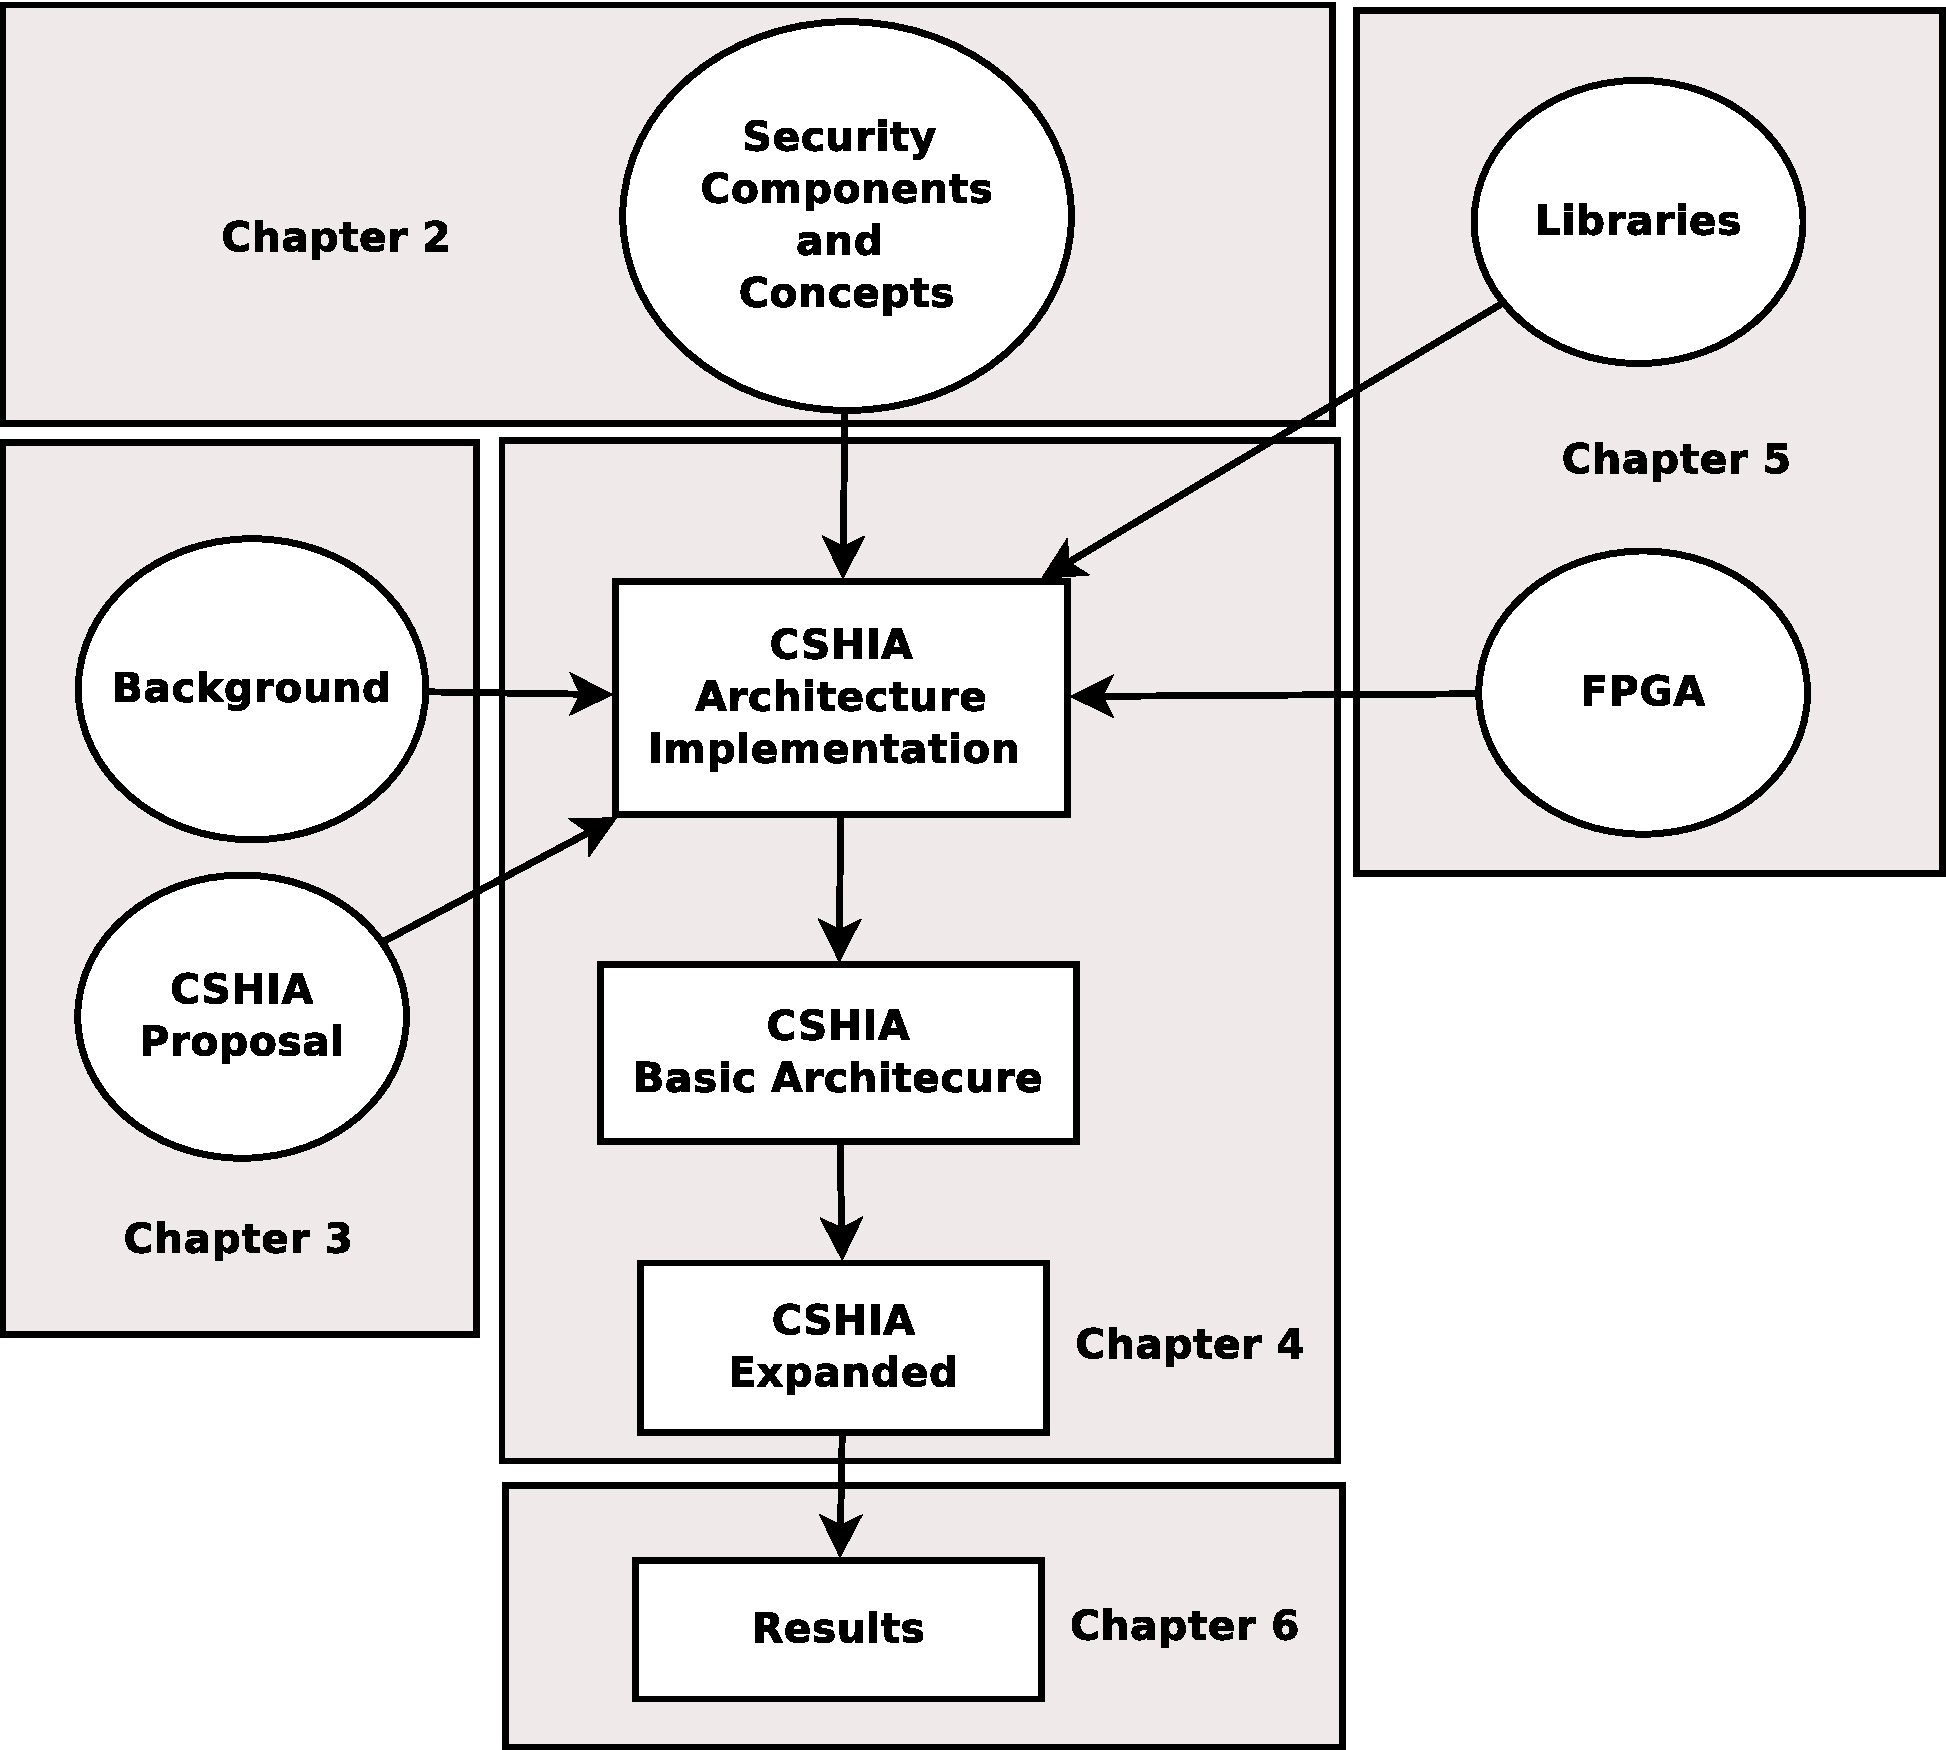
\includegraphics[scale=0.25]{figures/pdf/organization.pdf}
% 	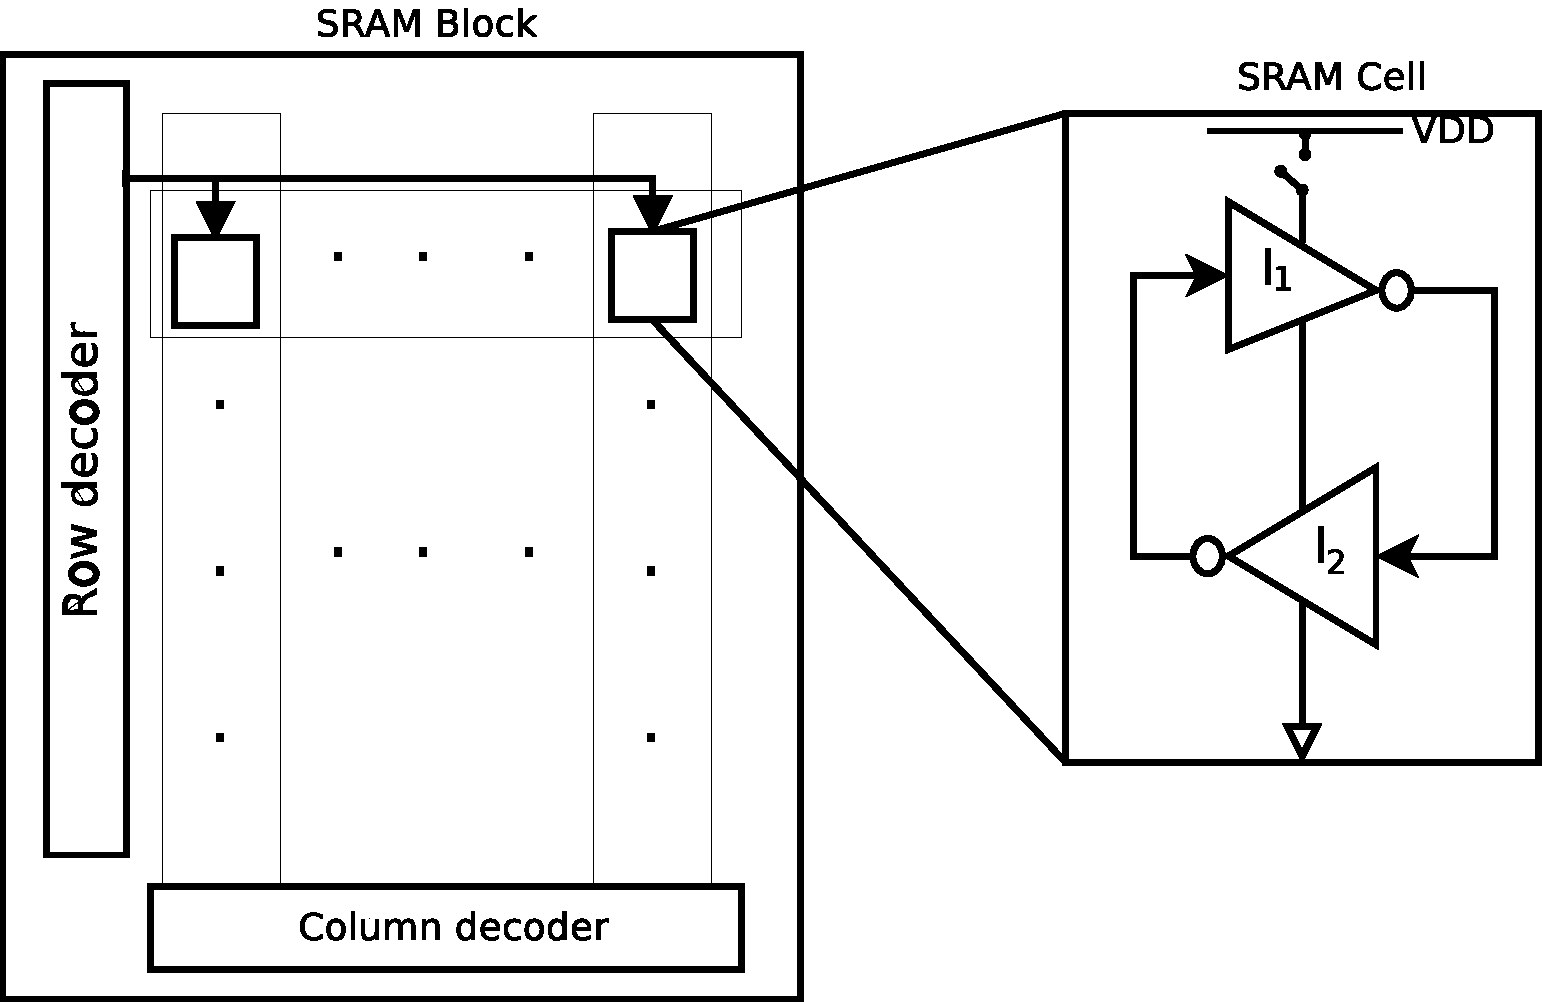
\includegraphics[width=\textwidth]{figures/pdf/spuf}
%	\caption{Visual organization of the dissertation.}
%	\vspace*{-9pt} 
%	\label{fig:orgvisual}
%\end{figure*}

%Security issues in embedded system are discussed in Section \ref{sec:Security-Issues-in-Embedded-Systems}. Section \ref{sec:CSHIA} describes the architecture. Section \ref{sec:Implementation} provides details about the implementation of \cshia~in the \leon's platform. Section \ref{sec:Experiments-and-Results} discusses experiments and results. A security analysis of the \cshia~implementation is presented in Section \ref{sec:Security-Analysis}. Section \ref{sec:Related-Work} discusses related work and Section \ref{sec:Conclusions} concludes this work.




\chapter{Fundamental concepts}
\label{chap:fundamental_concepts}  
%======================================================================
\section{Physical Unclonable Functions - PUFs}
\label{sec:pufs}
\pufs~are physical functions created to mimic random functions. Their inputs, called challenges, and outputs, called responses, are designed to have a unique relation for every \puf~instance. This is achieved by leveraging on imperfections resulted from fabricating electronic devices.

\subsection{PUF types}
\begin{figure*}[!ht]
	\centering
% 	\includegraphics[scale=0.45]{cshia}
	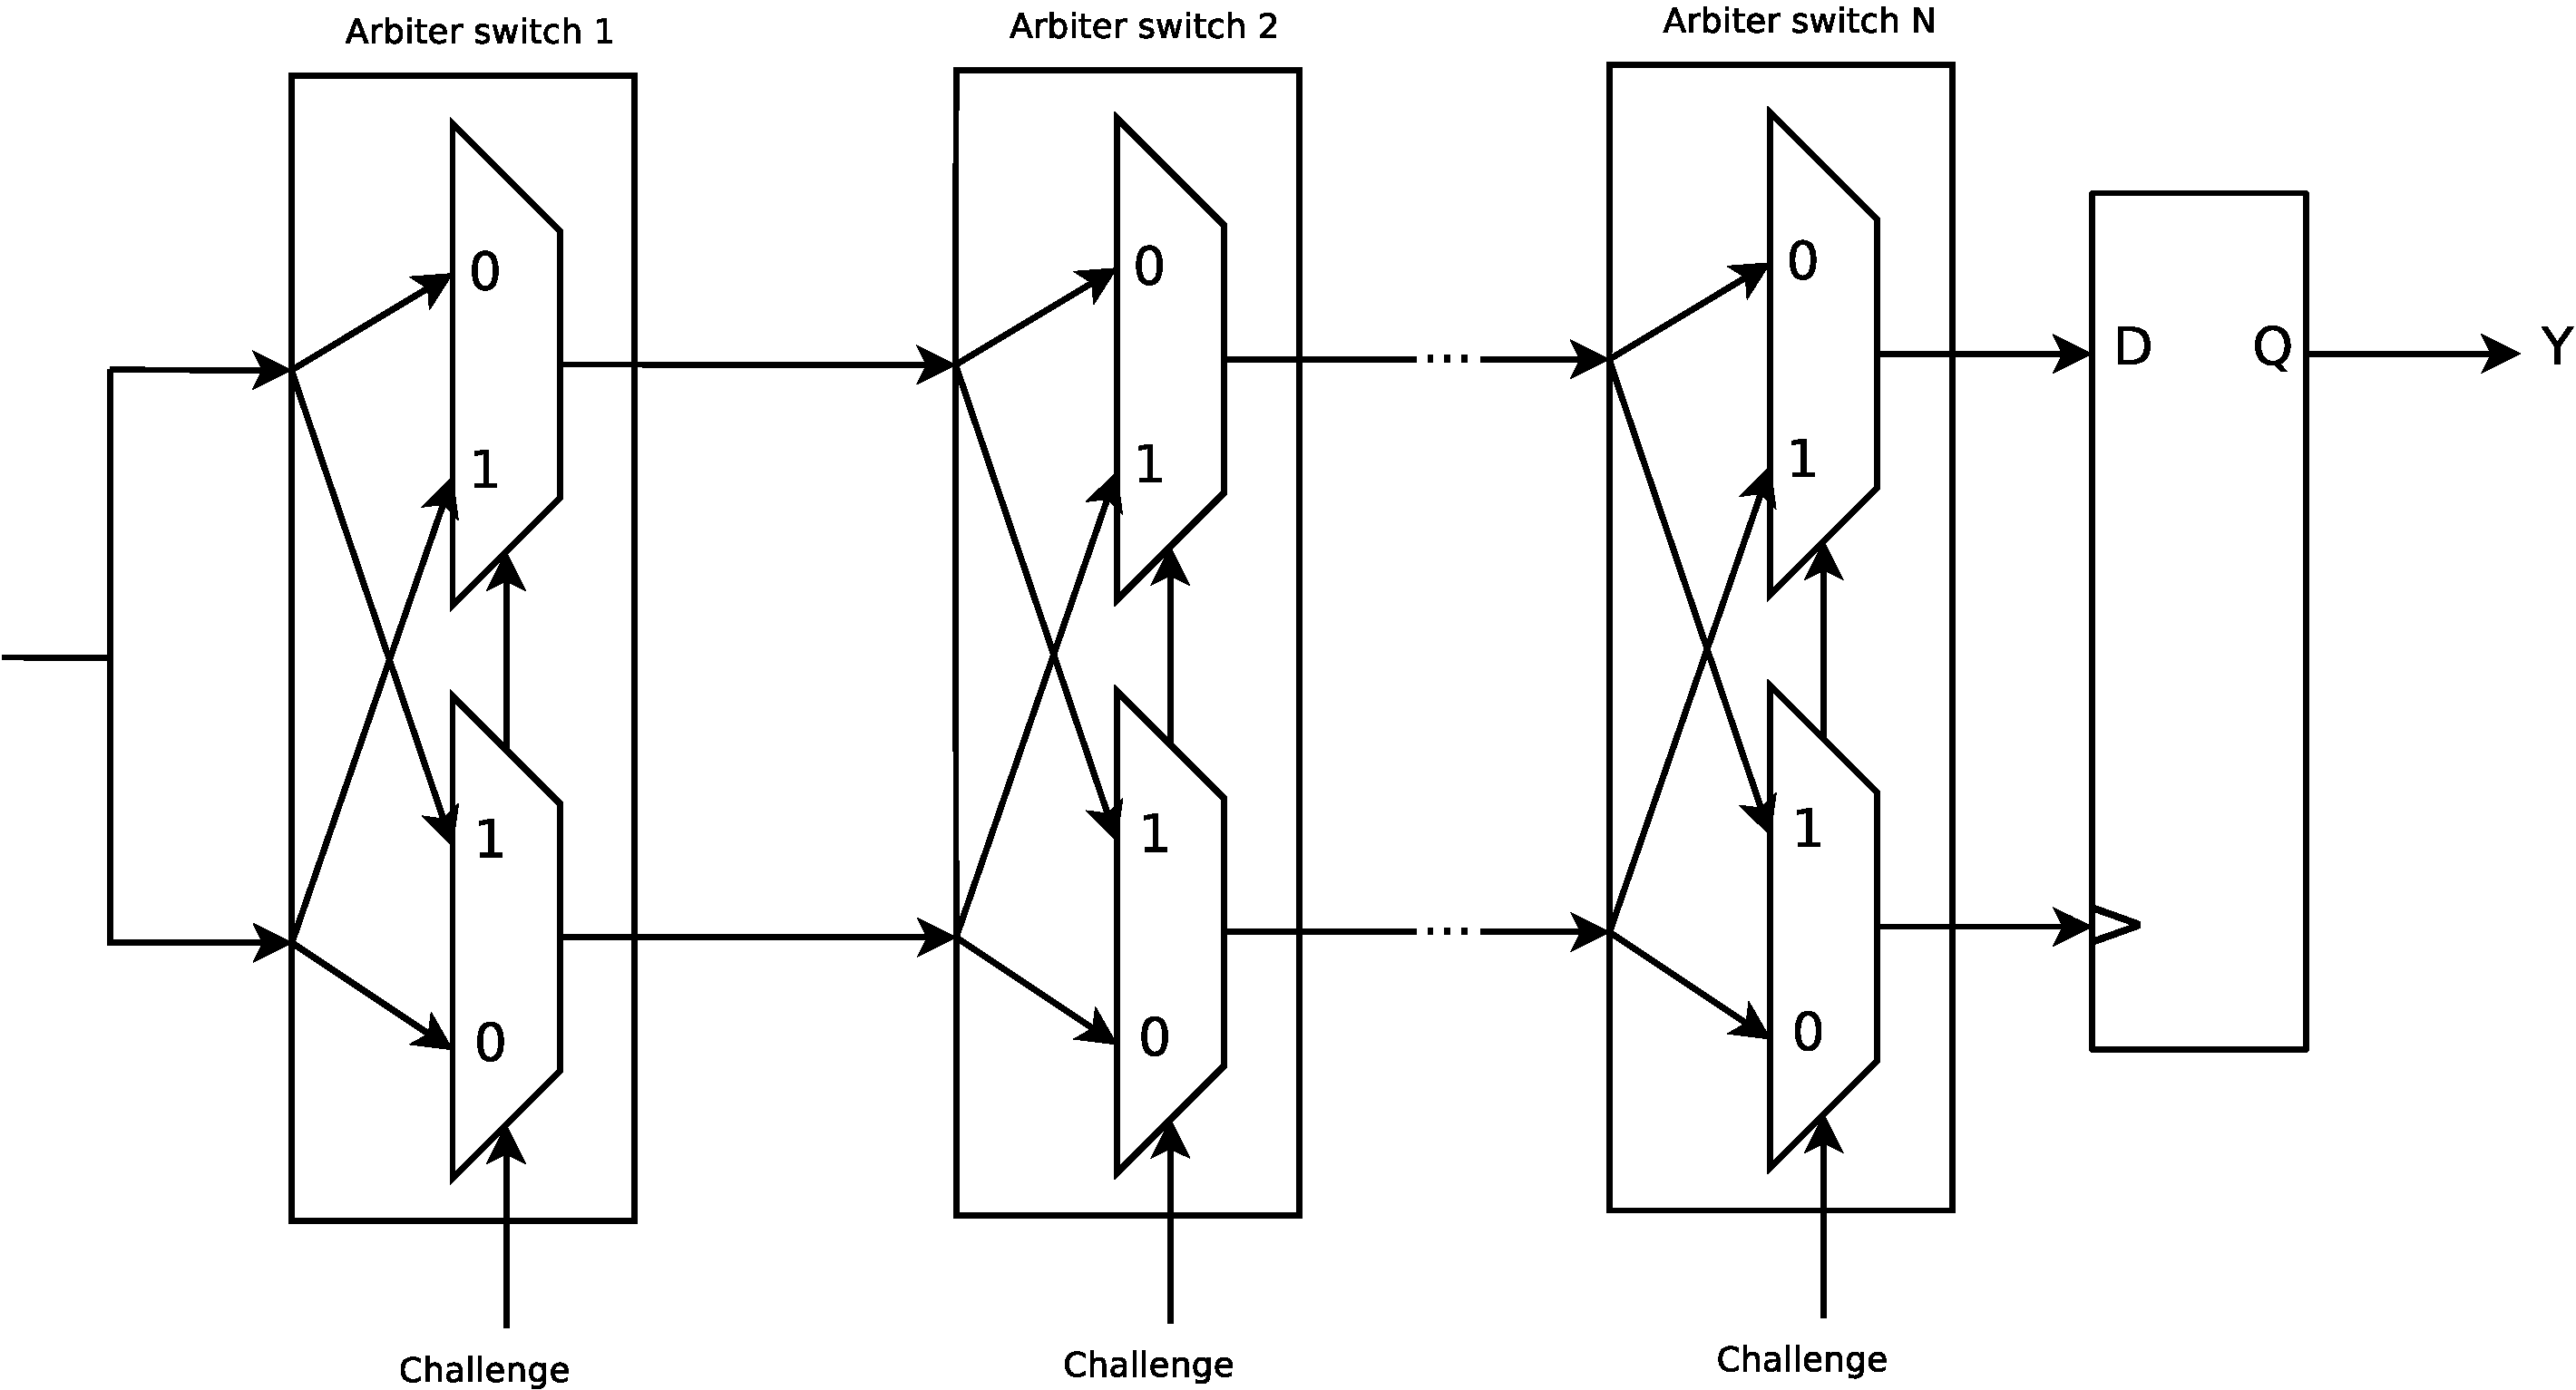
\includegraphics[width=\textwidth]{arbiter}
	\caption{The \cshia~architecture.}
%	\vspace*{-9pt} 
	\label{fig:cshia}
\end{figure*}

\subsection{PUF as a key}
When a system needs a key in hardware for any purpose, such as encryption, authentication or any other application, this key needs to be generated  and stored in hardware
\cite{puf-key-devadas-1278484}. The main advantage of using \pufs~as key generators is that they can produce keys at running time, this way, on-chip memories are not needed for key storage. Another benefit is that they are unclonable, meaning that even the manufacturer itself cannot produce two \puf~instances that will have the same set of Challenge-Response Pairs (\crps) \cite{Gassend2002:PUFs}.


%======================================================================
\section{Security Properties}
\label{sec:securityproperties}
In order to counter the attacks discussed above, a system designer need to employ mechanisms that implements three security properties: authenticity, integrity, and secrecy. Although these features can be implemented through software, the stringent nature of embedded systems demands solutions that consume few clock cycles and are not power consuming.
In the following, we discuss hardware implementation of those security features.

%---------------------------------------------------------
\subsection{Authenticity}
\label{subsec:Authenticity}
Suppose that an attacker wants to add \hisher~own code for execution in the embedded system or intends to move the data from one system instance to another. These attacks can be avoided by employing authentication mechanisms. In this solution, a key (or unique set of keys) is determined for each instance.
%TODO explain the instance more clear
Code \andor~ data are tagged using these keys during manufacturing (an enrollment phase). At run time, this key (or set of keys) is used to regenerate tags. Only a correct key value will be able to verify what was installed during manufacture. Therefore, an instance will not accept code or data that was not tagged using its own keys.

Before the introduction of electronic \pufs \cite{Gassend2002:PUFs}, these keys had to be inserted into the system  before they were made available to the users. To do so, keys are stored on chip using non-volatile memories and the manufacturer\slash{}vendor controlled the uniqueness of the keys in each instance. The main downsides of storing key permanently include: facilitating physical attacks \cite{Sadeghi2010:Security-PUFs}, and possibly increasing costs of production since it may demand integration of different technologies on the same chip.

%---------------------------------------------------------
\subsection{Integrity}
\label{subsec:integrity}
\ref{subsec:integrity}
Similarly  to authentication, integrity is ensured by tagging code and data with additional information such as memory address location \andor~timestamps. This prevents an attacker from tampering with a system by, for instance, moving instructions from their location in memory, setting different initial values of variables, etc. The level of integrity can be done for an entire program, memory pages, or memory blocks. 

Integrity can also be considered at the instruction sequence level, which we refer as Control-Flow Integrity (CFI). Hardware solutions for control-flow integrity usually require deep integration between hardware and software \cite{Davi2015:HAFIX}, that can result not only in changing the Instruction Set Architecture (\isa) \andor~the tool-chain, but also the processor's data path, as proposed in \cite{Gelbart2005:CODESSEAL, Kanuparthi2012:DynamicIntegrity}. Even though CFI protection is welcomed, many embedded system applications cannot afford the performance penalties and storage overhead inherently of this solution. For instance, in applications where user inputs are limited and \io~involves fixed amounts of data, an attacker has very little room to employ a buffer overflow or similar attacks prevented by CFI. However, integrity verification regarding blocks of code and data (as mentioned above) can avoid a variety of situations that go beyond run time attacks. For example, if an embedded system is unwatched, an attacker can upload a malicious code or modify the data in the external memory even if the system is not running. Integrity verification can prevent and indicate these violations before they reach the processor.


%---------------------------------------------------------
\subsection{Secrecy}
\label{subsec:Secrecy}

An embedded system can also use encryption to prevent exposure of code \andor~data stored in the external memory. Consequently, the processor can run these instructions and data only after decryption. Therefore, the major drawback of using encryption is the performance overhead that highly depends on which cryptographic primitive is employed \cite{Suh2007:PUFs}. In addition, secrecy only prevents that an attacker obtains the information, if it is not combined with a unique key or integrity verification, the system will be vulnerable to execute code of different system instances \andor~to suffer relocation and replay attacks\cite{Elbaz2009}.

\chapter{Related Work}
\label{chap:related_work}
%TODO


%SOC
%\soc~devices have a number of features which distinguish them from other traditional electronic solutions. Their dedicated nature allows the adoption of more intrusive protection, while posing challenging energy and performance requirements. Unfortunately, traditional security solutions based on typical cryptographic mechanisms (e.g. bus encryption)  can have a significant impact in device cost, energy efficiency and performance. One way to go around that is to consider approaches which enable a deep integration of device hardware-intrinsic features and program execution, as those offered by \pufs.

Qualitative analyses of \pufs~have already been done in the literature~\cite{Katzenbeisser2012} motivated by several applications such as cryptographic key generation~\cite{Suh2007, Bhargava2014} and true random number generation~\cite{Leest2012, Herrewege2013}. Unlike those works, which aim at evaluating the quality of a standalone \puf-inspired mechanism. %\new{On big conundrum on using \pufs~is how to prevent unintended bit-flips on responses used to compound the cryptographic key. An approach to deal with that is to use post-processing schemes like Fuzzy Extractors \cite{}. Despite the fact that Fuzzy Extractors be a simple and known circuits, they the weakest spot on the architecture and can leak the cryptographic key through side channel attacks. }

Most of the preliminary work on secure code execution aimed at keeping instructions and data secure from scrutiny, by using mechanisms like bus encryption. In~\cite{Elbaz2005}, Elbaz \etal~performed a comprehensive survey of bus encryption, where they describe many possible ways of using cryptographic algorithms in \soc~architectures, so as to ensure that no malicious instruction\slash{}data would be executed by the CPU. The major shortcoming of these solutions is the usage of on-chip secret key storage in non-volatile memories, which enable off-line key recovery attacks~\cite{towardshardwaresecurity2010}.

AEGIS, the secure processor proposed by Suh \etal~in~\cite{Suh2005}, employs \pufs~as a cryptography primitive to uniquely authenticate code and data in order to prevent both software and physical attacks. They present a toolchain for developing a secure software for their architecture which includes a secure operating system to manage different levels of memory protection. Although the presented toolchain does not require modifications in the processor architecture, it demands extensive changes in the \soc~architecture, in addition to changes in the compiler and operating system. Moreover, AEGIS \emph{does not} ensure full-time security from power-on to power-off; i.e. the system runs unprotected until the security kernel loads the system. In addition, physical attacks were neither evaluated nor simulated. Different circuits used in AEGIS, like \pufs~and post-processing schemes for key extraction such as Fuzzy Extractors, have been successfully attacked with side-channel \cite{Merli2011,Tajik2016:Photonic} and semi-invasive attacks \cite{Tajik2015:LaserAttack}. While semi-invasive attacks are hard to repeal, side-channel attacks have few known countermeasures \cite{Merli2013:Masking} that can be quickly adopted.


%A fine list of works in the literature has influenced this work. Their weaknesses and strengths, targeted systems, and construction helped us to make design choices to implement a proof of concept of \cshia. 
%Security 
%In 2003, Yang, Zhang, and Gao \cite{Yang2003:XOM} proposed an improved version of \xom, an architecture for digital copyright protection. The architecture provides authenticity through a pairwise private\slash{}public key. Every instance of a \xom~architecture has a unique private key. Secrecy is provided by encrypting software using specific symmetric keys chosen by the software vendor. These keys are encrypted using \xom's public key and therefore only the instance that has the correspondent private key will be able to execute the software. \xom~provides integrity protection by hashing memory blocks, but it only prevents spoofing and splicing. Replay attacks are left uncovered. The differential of \xom~is to isolate programs in compartments, which have their own tags and keys. Due to this isolation, new instructions had to be added to the processor in order to relax constraints of architecture. For example, to enable sharing data between isolated programs. From the point of view of targeted market, \xom~is suitable for very high end embedded systems or above since they simulated their architecture using a processor capable of out-of-order execution and \xom's performance highly depends on the existence of second-level cache (\ltwo) and its size. Finally, area overhead is not estimated, implementation is through simulation, and the averaged performance slowdown is 16.76\% on the tested benchmarks, however, they were able to reduce this slowdown to 1.28\% implementing an additional cache memory. 

%The first architecture that proposed to use \pufs~for key generation was \aegis, the work presented by Suh \etal~in \cite{Suh2005:AEGISImplementation}. \aegis~is a tamper-resistant and tamper-evident architecture. Meaning that it hinders tampering threats, but the system still indicates if an attacker successfully overpasses the security features. \aegis~is a complete solution in which not only new instructions are provided, but also system calls, security modes, and different divisions of memory into new regions. It can securely run even under an untrusted operating system. \aegis~provides a \mt~to prevent replay attacks and uses a small cache to store nodes and reduce performance penalties. All this security comes with downsides such as an almost 100\% area increase in comparison to the processor baseline, and the modification of the entire toolchain: compilers, operating systems, and even programs. Due to the complexity of the architecture, targeted systems are preferable high-end embedded systems or above. Although the authors are not very clear about overall performance penalties of the architecture, when they used their full protection mode and an architecture configuration consisting in 32 KB instruction\slash{}data cache and 16 KB \mt~cache, the worst benchmark performance overhead was 3.3\%. However, when the architecture configuration is 4 KB instruction\slash{}data cache and 2 KB \mt~cache, the same benchmark has a performance overhead of 73.1\%.

%Following \aegis~in 2005, Then SecBus 2009
%Liu 2013



%Rogers, Milenković, and Milenković presented in 2007 a secure architecture \cite{Rogers2007:LowOverhead}. Different from the previous works described above, they truly focused on embedded system since they assume that processors would not have second-level cache memory (\ltwo), but would present a separated \lone~into data and instruction memories. Their architecture provides integrity and secrecy for memory blocks of instructions, and data integrity is not discussed. The architecture uses virtual address to compound encrypted blocks, in order to thwart splicing attacks, they came up with a interesting solution of encrypting an unique \puf-generated (or thermal-noise generated) key together with the program this key authenticated. Thus, when two programs present a collision between virtual addresses, an attacker will not be able to switch programs because their key will be different. Although their architecture was only simulated, they estimated a power consumption overhead over the baseline system. Setting up a simulation of an ARM processor with small instruction \lone~cache of 1 KB resulted in a power consumption overhead as high as twice the baseline's value. In terms of performance penalties for the tested benchmarks, the results also were very detrimental for a small instruction \lone, achieving an overhead of 2 times greater than baseline's performance, and becoming negligible for a 8 KB instruction cache in the best scenario. At last, for a standard memory block of 256 bits, their storage overhead reached 50\% of the main memory, which is high. 
In 2009, Vaslin \etal~proposed a security approach for off-chip memory in embedded microprocessors \cite{Vaslin2009:OTP}. Vaslin \etal~used the One-Time-Pad (\otp) scheme to provide integrity and secrecy. Their architecture encrypts a timestamp, the memory address and a padding value using \aes. Then, this encrypted content is combined with the cache line. Because they used memory address and timestamp, relocation and replay attacks are thwarted. However, to inhibit spoofing attacks, memory blocks need tags and Vaslin \etal~proposed using \crc32. One critical point is that their architecture needs not only an internal timestamp memory but also a \crc32 memory. That led to internal memory of at least 18.8\% of the size of main memory. Nonetheless, Vaslin \etal's architecture was able to achieve a worst-case performance impact of 10\% in the tested benchmarks. However, the area overhead in the \fpga~tested almost tripled.

%\fedtic, the 2010 work of Hong and Guo \cite{Hong2010:FEDTIC}, is an architecture for integrity verification and secrecy for embedded systems. Their main contribution is a single engine that uses one \aes~hardware instance for encryption, decryption, and tagging of cache lines. As in \cite{Vaslin2009:OTP}, a stamp is generated for each memory block write back, which prevents replay attacks. However, instead of a one-time-pad scheme, Hong and Guo used \aes~in output feedback mode, which allowed them to use shifted encrypted blocks to compose a tag. In terms of achievements, for a 512 bit cache lines, their external memory overhead was less than 7\% and for the tested benchmarks a maximum internal memory for timestamps needed was 5 KB. It should be noticed that this internal memory is not a cache and thus will increase with the program size. The average performance penalty was 7.6\% and the maximum 30.72\%. Their evaluation used a combination of simulation and \fpga~implementation.

Bobade and Mankar presented in \cite{Bobade2015:SecurityFPGA} a secure architecture for embedded system. Their architecture provides integrity and secrecy through an Elliptic Curve Cryptographic engine. The main difference regarding the other architectures presented here is that they use the timestamps as private keys. Thus, cache lines are encapsulated with their address and time stamp (for integrity verification purpose), and then encrypted with the public key to be stored in external memory. As the timestamps are stored in internal memory, the decryption can be done with reprocessing the pair private\slash{}public key and the integrity is ensured by the correct decryption of the triad encapsulated: data, address, and time stamp. Although Bobade and Mankar synthesized their architecture for a {\fpga}S, they only simulated the architecture and did not use any benchmark. Nonetheless, they computed the overhead of slices and \luts~over their baseline processor, which was over 76\%. Memory overhead was 25\%. Also, they estimated power increment over baseline. Despite the dynamic power more than doubled in all processor's frequency simulated, the static was kept stable.

Recently, Sepulveda, Wilgerodt, and Pehl in \cite{Sepulveda2018:CSHIA} proposed a Multi-Processors System-on-Chip that provides memory integrity and authenticity through \pufs. The proposed architecture innovates by targeting multi-processors. %They also used \siphash~to provide memory blocks integrity tags to protect against all three significant threats we have discussed before. 
One key difference in their replay attack solution is that they use session tokens instead of timestamps. While that is an innovative way, it may not be sufficient to protect against replay attacks, since tokens are updated during idle periods and booting time. Thus, in a long period of execution, in which a specific memory block can be written back multiple times to memory, an attacker might mount a replay attack. One interesting point is that Sepulveda \etal argues that \cshia~needs profound modifications in \soc~and \cpu. However, we believed that this work demonstrates that only minor modification is needed and they are all transparent to the core and does not affect how it works. It is also essential to notice that the authors used a similar Code-offset Fuzzy Extractor \cshia~had employed initially, which, as discussed in the previous section, is less secure than the one used in \cshia~in terms of entropy reduction of the key. Finally, they estimated area and power of the components of their architecture and did performance evaluation which, by computing an average degradation, was 5.6\% on the tested benchmarks.

Table \ref{tab:related-work} presents a summary of the advantages and drawbacks of \cshia~and related works. A fair comparison of performance among the works is quite hard to be performed, due to a variety of benchmarks, baseline cores, choice of platforms, among others. However, a qualitative analysis of design choices can still be done, as discussed in section \ref{chap:cshia_architecture}. For instance, \pufs~have continuously been claimed to be a better solution for key generation than storing on-chip key. In that regard, \cshia~is more advantageous than those that did not use them. All the mentioned related works have a higher abstraction level, in this work, we disclose the implementation details and design tradeoffs of \cshia. 

%security related 
%Moreover, we carefully analyzed major threats presented in the literature in order to propose a secure employment of a \puf-based key. Because embedded system applications can have a very specific nature, our concern since the beginning was to propose a flexible architecture, which is characterized by its additional bus for the \ptagmem~and the choice between timestamps or \mt~as replay attack solution. Thus, although we were not able to precisely estimate power and area, we believe that we presented a solid solution for the security of embedded systems. 





%\begin{sidewaystable}
\begin{table*}[!ht]
	\center
	\caption{Summary of Related Works in comparison with \cshia.}
	\label{tab:related-work}
	\footnotesize
	%\begin{tabular}{cp{1in}p{2in}p{2in}}
	%\begin{tabular}{cppp}
	%\resizebox{\textwidth}{!}{\begin{tabular}{cccc}
     \resizebox{\textwidth}{!}{\begin{tabular}{cp{1in}p{2in}p{2in}}
		\hline
			Work & Target Architecture & Advantages & Drawbacks \\	
		\hline
		%\hline
		%	\xom & High-End embedded systems and above & Program isolation & Does not provide protection against replay attacks. \\
		\hline
			\aegis\cite{Suh2005} & High-End embedded systems and above & A complete solution & Integration with standard products can be difficult due to modification imposed to the whole toolchain. \\
		%\hline
		%	\cite{Rogers2007:LowOverhead} & Embedded Systems & Program Isolation & High memory overhead. \\
		\hline
			\cite{Vaslin2009:OTP} & Embedded Systems & Uses \aes~in \otp~mode combined with \crc32 to provide integrity with low on-chip memory overhead. & High area overhead in a \fpga~implementation. \\
		%\hline
		%	\fedtic & Embedded Systems & Uses one \aes~component to encryption, decryption and authentication & Can impose large on-chip non-volatile memory. \\
		\hline
			\cite{Bobade2015:SecurityFPGA} & Embedded Systems & Security is based on public-key cryptography. & No performance evaluation.\\
		\hline
			\cite{Sepulveda2018:CSHIA} & MP\soc & First \puf~based secure architecture for multiple cores. & Does not estimate area and power increment in regard to the baseline system.\\
		\hline
			\cshia & Embedded Systems & Design Flexibility. & Does not provide concrete estimate of area and power. \\
		\hline
	\end{tabular}}
	%}
%	\vspace*{-12pt}
%\end{sidewaystable}
\end{table*}

\chapter{CSHIA  Architecture}
\label{chap:cshia_architecture}



  %\system, illustrated in Figure \ref{fig:system}, is a processor architecture which aims at providing secure code execution by means of \puf-based authentication of cache lines. The central idea behind \system~is a \puf-Tag (\ptag) Memory, which runs in parallel with the system main memory (Figure \ref{fig:system}). Each entry in the \ptag~Memory stores an authentication code of a cache line generated by a \puf-based device located on-chip.
  
%   \begin{figure*}[!ht]
% 	\centering
% 	\includegraphics[scale=0.35]{cshia}
% %	\vspace*{-12pt} 
% 	\caption{A system overview of the \system~system.}
% %	\vspace*{-9pt} 
% 	\label{fig:system}
% \end{figure*}

  %\new{In comparison to traditional architectures, \system~includes two main modifications: The \textit{Secure Engine} (\tagsystem), which includes the \textit{PTAG Generator} (\ptaggen, Figure \ref{fig:ptaggen}); and the \textit{Security-Cache} (\seccache) that controls bus traffic between the processor and the \textit{Memory Controller} (\mctrl). Other two new architectural components are also required to complete the \system~design, the \textit{\ptag~Memory} and the \textit{PTAG Bus}. In a few words, when the processor requires\slash{}sends data\slash{}instructions to the \mctrl, the \seccache~sends the related cache line to the \tagsystem~for computing\slash{}validating its \ptag. Notice from Figure \ref{fig:system} that the \ptag~bus runs in parallel to the system buses, and thus no program can directly read the \ptag~Memory, since neither the processor nor the \mctrl~are aware about the \seccache.}


  % \subsection{\ptaggen~Operation}
  % \label{subsec:ptaggenOpr}

  % \new{The \tagsystem~controls the \ptaggen~based on the information delivered by the \seccache. This information is generated from bus transactions (Memory READ, Memory WRITE and I\slash{}O) between the processor and the memory controller, and which the \seccache~controls. Next, each \ptaggen~action is explained in regard to bus transactions.}
  
  %     \begin{figure*}[!ht]
	 %  \centering
	 %  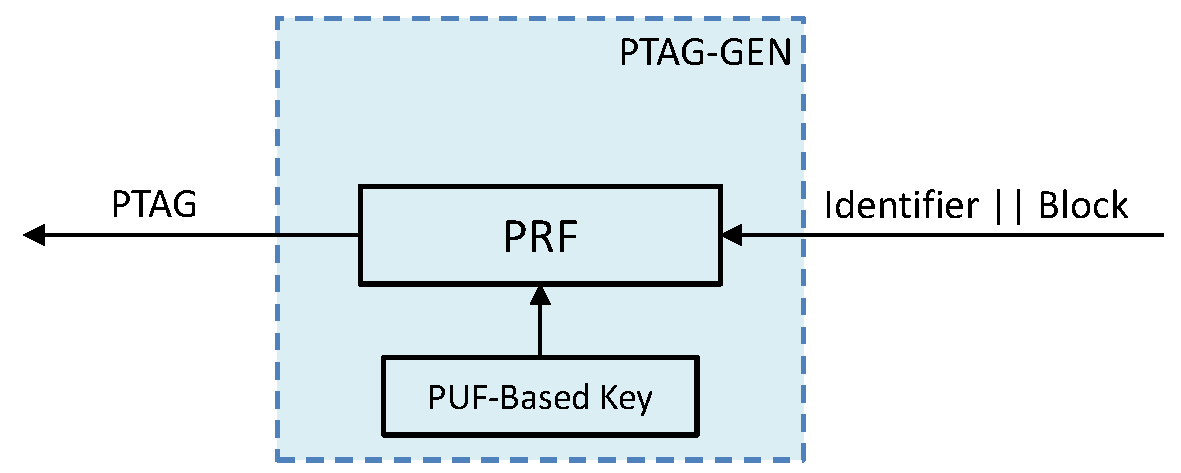
\includegraphics[scale=0.4]{ptaggen}
	 %  \caption{The \ptaggen~during \ptag~Generation (write) and \ptag~Verification (read) operations.}
  % %	\vspace*{-9pt} 
	 %  \label{fig:ptaggen}
  % \end{figure*}
  

	 %  \subsubsection{\ptag~Generation (memory write)}
	 %  \label{subsubsec:ptag-generation}
  % \new{During a write operation, the \seccache~passes data\slash{}instruction cache lines to the \tagsystem~and the \ptaggen~computes \ptags~and stores it into the \ptag~Memory. A \textit{Pseudorandom Function} (\prf) \cite{Goldreich2004} module is used to generate the \ptag~and takes as input the concatenation ($||$) of the cache line bits and the base address of the cache line provided by the core (see Figure \ref{fig:ptaggen}). In order to ensure uniqueness, the \prf~is configured using a \textit{unique-per-device key}. This key is produced by the intrinsic hardware features of a~\puf. Such authentication tag is specific to the core running that specific cache line, as ~\puf~outputs are dependent on the statistical variations of the manufacturing process, and are unique to each processor~\cite{Katzenbeisser2012}. Hence identical cache lines running on different processors will produce different \ptag~values for the same inputs. Notice that only code in the cache, for which integrity has been ensured, will be able to write to memory.}
  


	 %  \subsubsection{\ptag~Verification (memory read)}
	 %  \label{subsubsec:ptag-verification}
  % \new{During a read operation, the \seccache~passes data\slash{}instruction cache lines to the \tagsystem~and the \ptaggen~computes \ptags~for verification. As shown in Figure~\ref{fig:ptaggen}, during a read operation the cache line base address produced by the core is appended to the cache line contents read from memory and the result is fed to the \prf~module. The \ptag~produced this way is compared to the PTAG read from memory for equality. If the previously stored \ptag~and the recently computed value do not match, a \textit{Non-Maskable Interrupt} (NMI) is generated to the core (called \ptagnmi), as code\slash{}data integrity may have been violated. As shown in Figure \ref{fig:system}, in order to hide \puf~latency, the data\slash{}instruction is sent to the respective cache (I\$ or D\$) at the same time that \ptag-GEN computes the \ptag~for that cache line and compares it to its \ptag~previously stored into the \ptag~Memory.}

	 %  \subsubsection{Handling I\slash{}O}
	 %  \label{subsubsec:io}
  % In modern computer systems, I\slash{}O operations store data directly into specific memory regions through DMA mechanism. Thus, it is not possible to trust such memory regions and \system~does not ensure their integrity and authenticity. Software should first perform authentication of I\slash{}O data in a higher abstraction layer and then copy it to secure areas where the \system~can ensure integrity and authenticity.


%\mario{never start a chapter with a figure, Add an introduction about what is going to be explained in  this chapter }





\section{Overview}
\label{sec:overviewarch}

%\mario {cite Caio thesis, make clear each contribution}
\cshia~was originally proposed in \cite{Hoffman2015} as an architecture for \iot. However, we believe that \cshia~fits in a broader class of embedded system applications that can benefit from its nice security features. Many embedded system applications do not need secrecy\slash{}confidentiality, but strongly require code and data authenticity and integrity. 
%\augusto{This is a detailed version with Caio  contribution   in a higher level, this work is about just authenticity so it would be better to  get the version to TECS and  talk about the  improvements made by caio and cite his thesis, i just dont know in which part }
\begin{figure}[!ht]
    \centering
%     \includegraphics[scale=0.45]{cshia}
    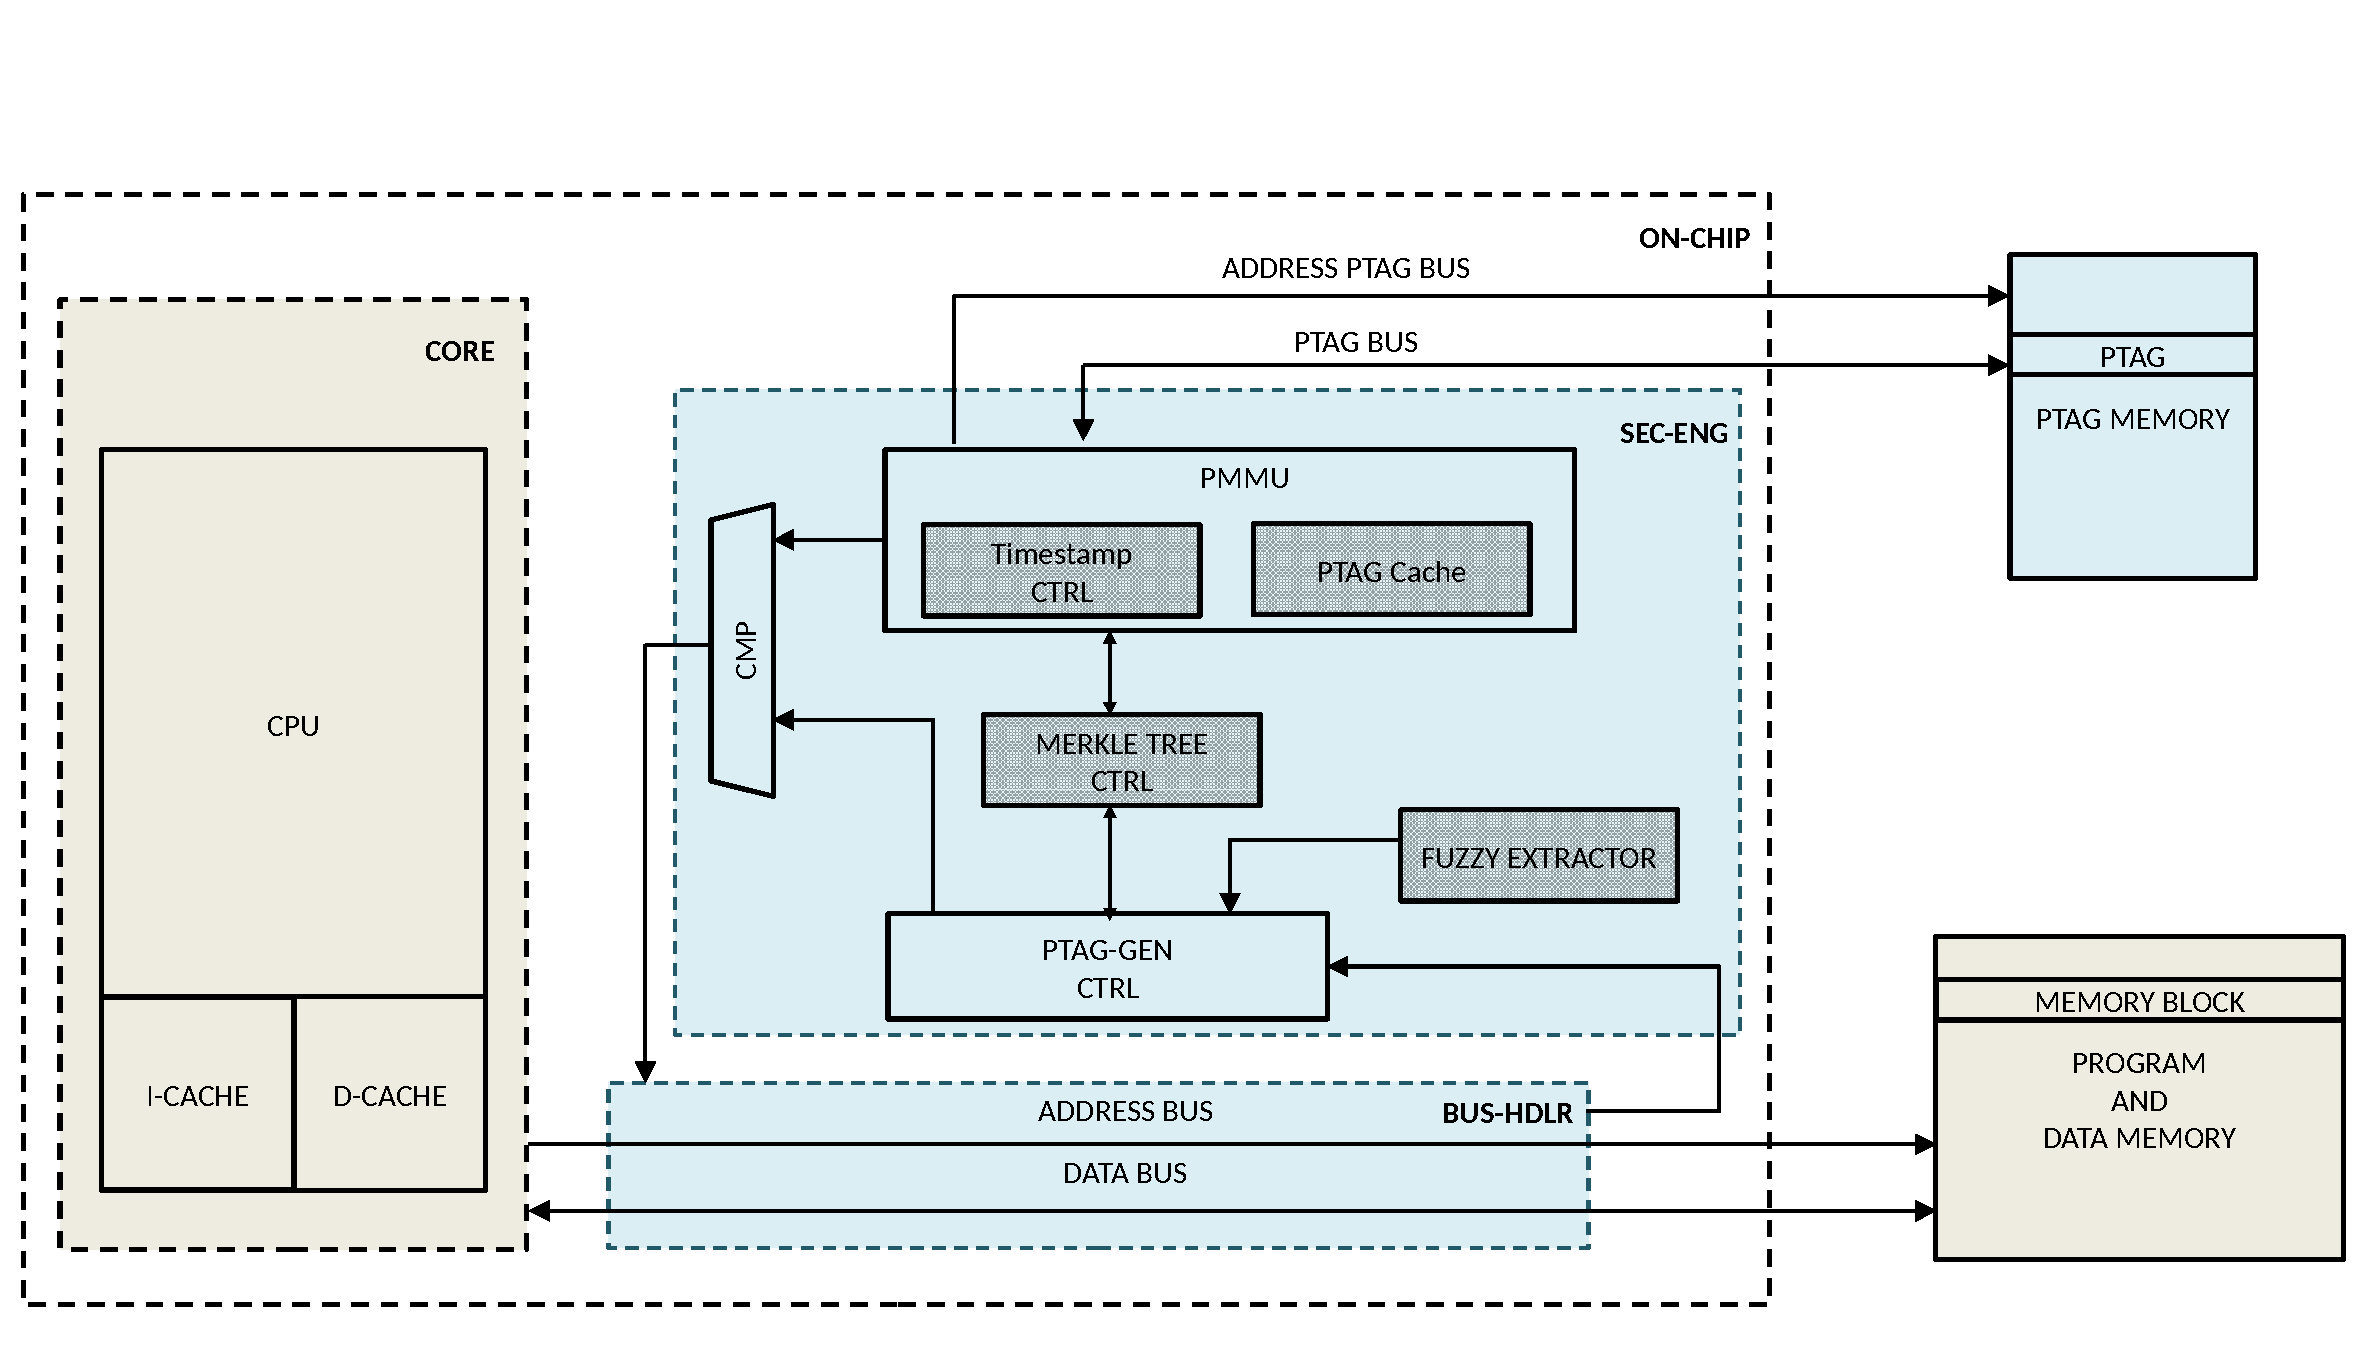
\includegraphics[width=\textwidth]{figures/pdf/CSHIA_detailed_caio_expansion.pdf}
    \caption{The \cshia~architecture.}
%    \vspace*{-9pt} 
    \label{fig:cshia}
\end{figure}
%\begin{figure*}[!ht]
%    \centering
%     \includegraphics[scale=0.45]{cshia}
%    \includegraphics[width=\textwidth]{figures/pdf/cshia.pdf}
%    \caption{The \cshia~architecture.}
%    \vspace*{-9pt} 
%    \label{fig:cshia}
%\end{figure*}
Using the original work with some architectural elements modified to provide stronger security features, the first LEON3 \fpga~ based implementation of \cshia was realized. This section focus on presenting the \cshia~implementation components and how they work to provide authenticity and integrity. Figure \ref{fig:cshia} illustrates the basic components required for \cshia~ to work: 
\begin{itemize}
    \item One core that in this implementation is a LEON3 processor;
    \item The \cshia~ components:
    \begin{itemize}
        \item \ptag~ Memory Management Unit (\pmmu)
        \item Bus Handler (\handler)
        \item Security Engine (\seceng) 
    \end{itemize}
    \item One external memory that contains instructions and data;
    \item One interconnection bus using \amba.
\end{itemize} 


\section{\amba}
\label{sec:amba2}
\begin{figure}[!ht]
    \centering
    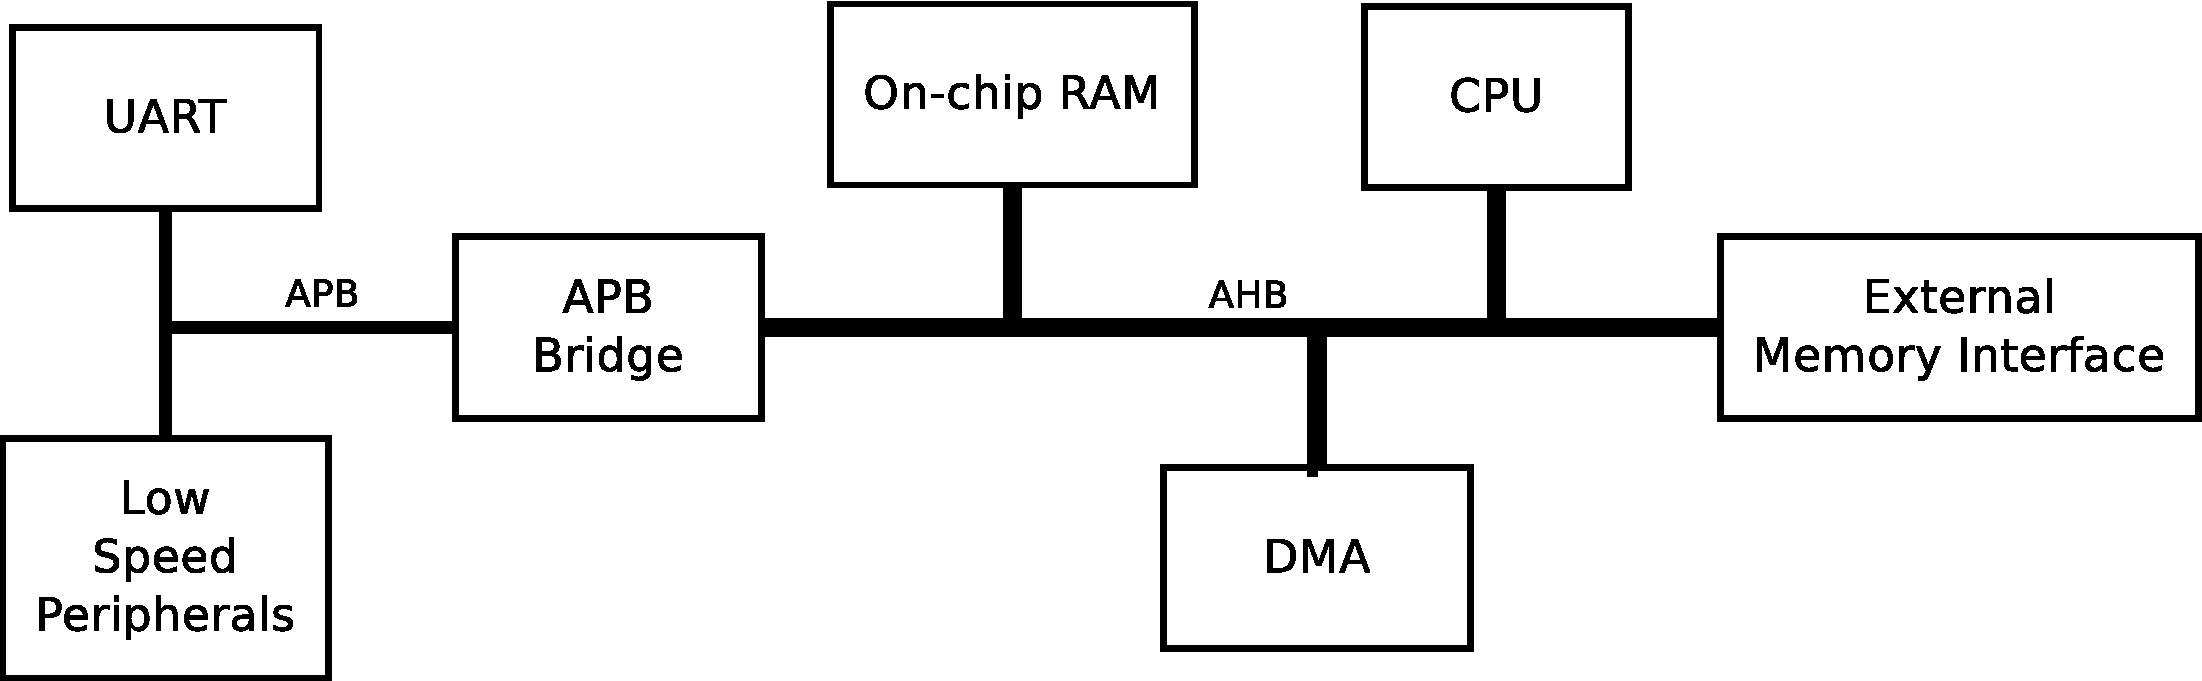
\includegraphics[width=1\textwidth]{figures/pdf/typical_amba_new.pdf}
    \caption{Typical \amba~ system , with a CPU , DMA and other low bandwidth peripherals. }
    \label{fig:general}
\end{figure}

The BUS used in the LEON3 processor is the Advanced High-performance Bus (AHB), where on-chip memory and other peripherals also reside. This bus provides a high-bandwidth interface between the elements connected to it, also, located on the bus is a bridge to the lower bandwidth APB, where most of the peripheral devices in the system are located. Figure \ref{fig:general} exemplify a traditional AHB utilization.

\amba~ AHB implements the features required for high-performance, high clock
frequency systems including:
\begin{itemize}
 \item {burst transfers}
\item {split transactions}
\item {single-cycle bus master handover}
\item {non-tristate implementation}
\item {wider data bus configurations (64/128 bits).}
\end{itemize}

 
\subsection{\amba~ AHB operation}

\begin{figure}[!ht]
    \centering
    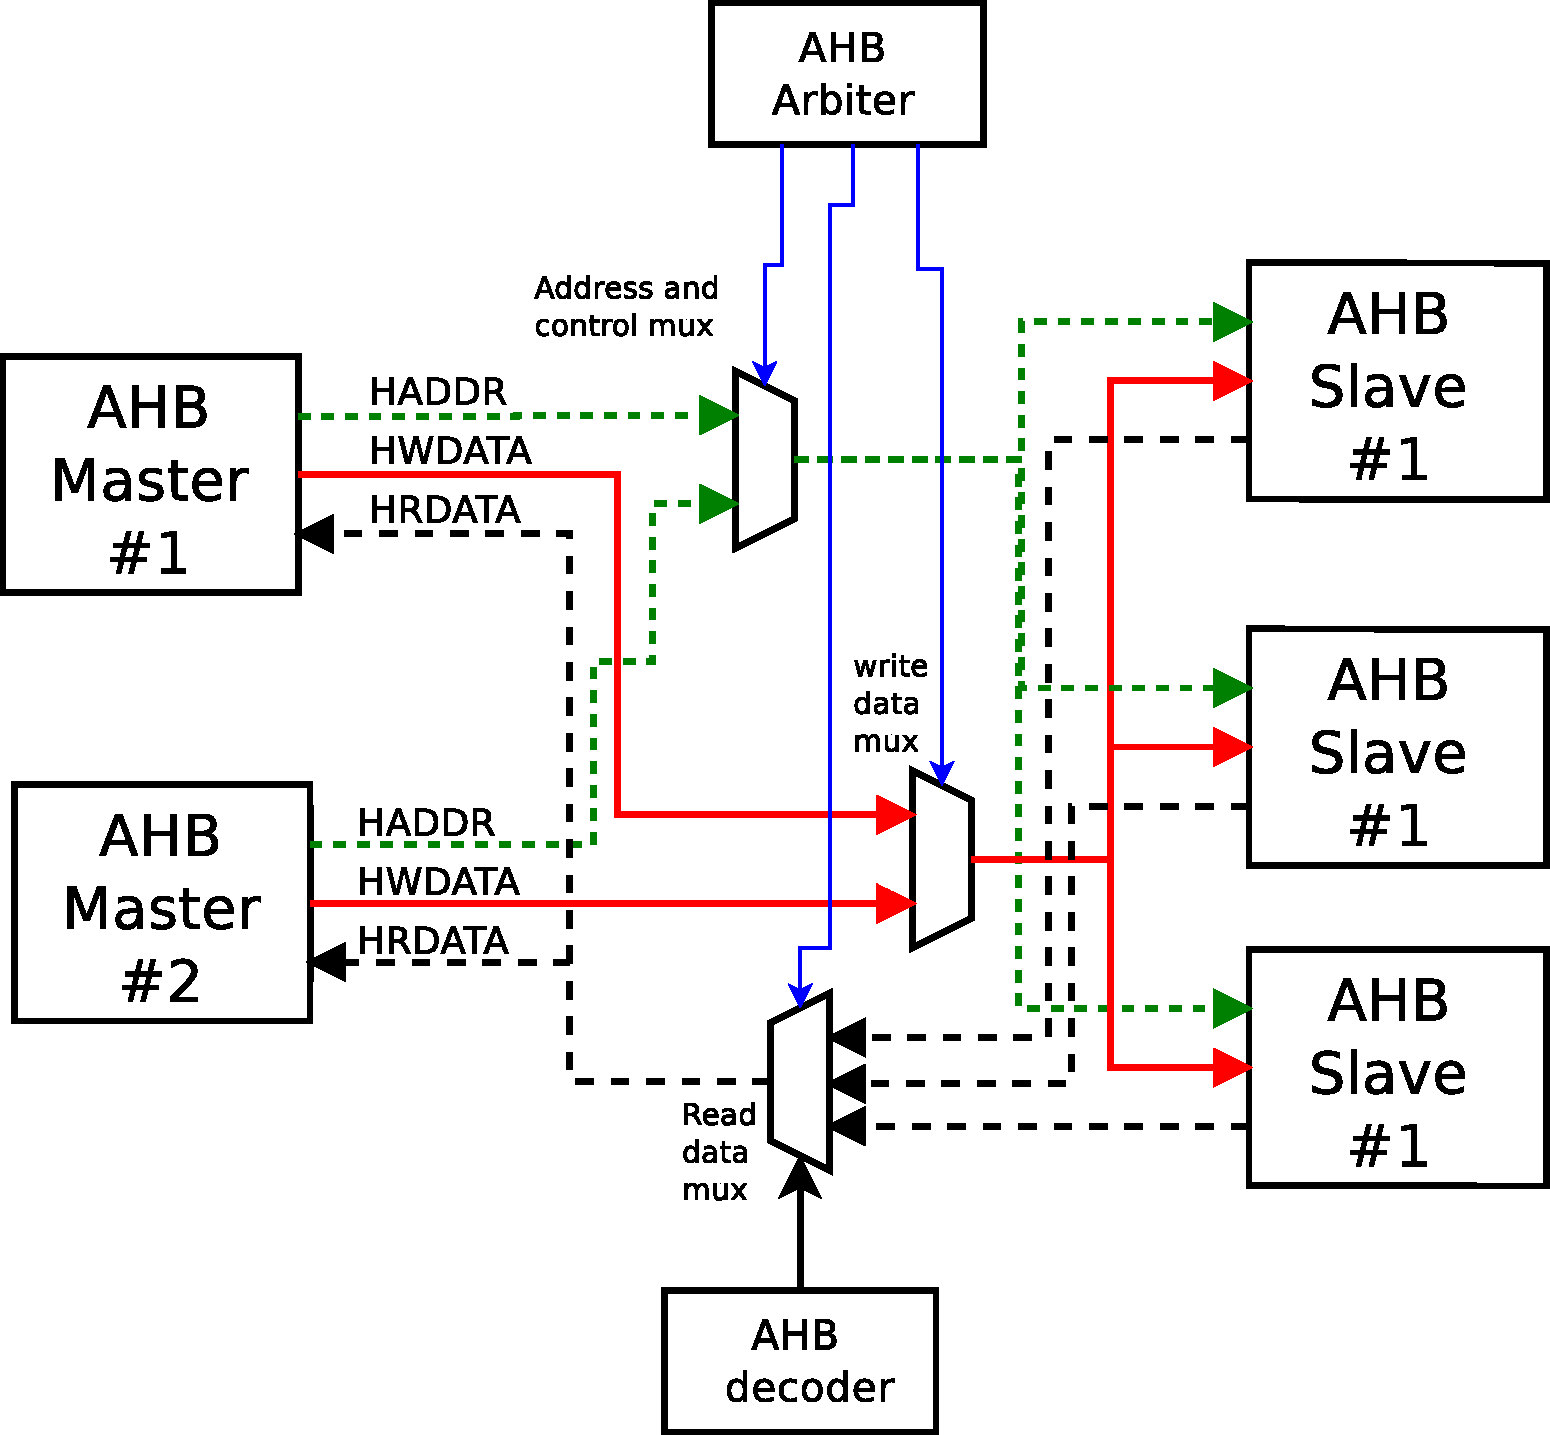
\includegraphics[width=0.7\textwidth]{figures/pdf/amba2_arbiter.pdf}
    \caption{Overview  of the \amba~ Organization, with the arbiters masters and slaves distribution.}
    \label{fig:internorg}
\end{figure}

The previously described \amba~ components are seen by the bus as masters and slaves, as depicted in Figure \ref{fig:internorg}, where, for instance, the CPU is an \amba~ master and the on-chip RAM is a slave. Who decides the priorities and decode all access is the \amba~ arbiter, which will be described further.

Before an \amba~ AHB transfer, from now on just referred to as transfer, can commence the bus master must be granted access to the bus. This process is started by the master asserting a request signal to the arbiter. Then the arbiter indicates when the master will be granted use of the bus. A granted bus master starts a transfer by driving the address and control signals. These signals provide information on the address, direction and width of the transfer, as well as an indication if the transfer forms part of a burst. Two different forms of burst transfers are allowed:
\begin{itemize}
\item incremental bursts, which do not wrap at address boundaries
\item wrapping bursts, which wrap at particular address boundaries.
\end{itemize}

A write data bus is used to move data from a master to a slave, during a read data bus
is used to move data from a slave to a master.
Every transfer consists of:

\begin{itemize}
\item an address and control cycle
\item one or more cycles for the data.
\end{itemize}

\begin{figure}[!ht]
    \centering
    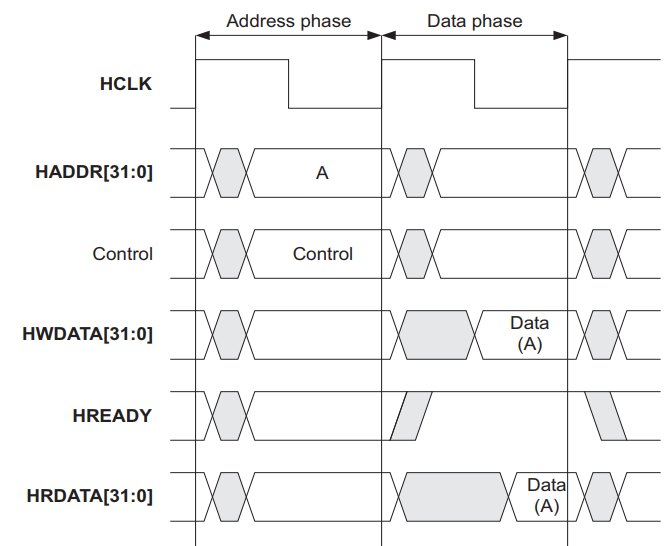
\includegraphics[width=0.4\textwidth]{figures/others/simple_ahb_transfer.png}
    \caption{AHB basic transfer with one cycle for address and control and one or many for data.}
    \label{fig:basic_ahb_transfer}
\end{figure}


In the address and control cycle, the address cannot be extended, and therefore, all slaves must sample the address during this time. The data, however, can be extended using the HREADY signal. When LOW these signal causes wait states to be inserted into the transfer and allow extra time for the slave to provide or sample data, as can be seen in Figure \ref{fig:basic_ahb_transfer}. During a transfer, the slave shows the status using the HRESP response signal where the  following values are used:

\begin{itemize}

\item  {OKAY -} The OKAY response is used to indicate that the transfer is progressing normally and when HREADY goes HIGH this shows the transfer has completed successfully.
\item {ERROR -} The ERROR response indicates that a transfer error has occurred and the transfer has been unsuccessful.
\item {RETRY and SPLIT  -} Both the RETRY and SPLIT transfer responses indicate that the transfer cannot complete immediately, but the bus master should continue to attempt the transfer. In normal operation, a master is allowed to complete all the transfers in a particular burst before the arbiter grants another master access to the bus. However, in order to avoid excessive arbitration latencies, it is possible for the arbiter to break up a burst and in such cases, the master must re-arbitrate for the bus in order to complete the remaining transfers in the burst.
\end{itemize}


\subsection{\amba~ Components}
%\augusto{say that we are reducing the scope to what was used in the design }
These \amba~ components are a  subset of the entire \amba~ features, the focus of this sections is to provide the basis to understand of the signals and work required for the \cshia~implementation, for a full reference please check \cite{ARMAMBA2}.

\subsubsection{Masters}
\begin{figure}[!ht]
    \centering
    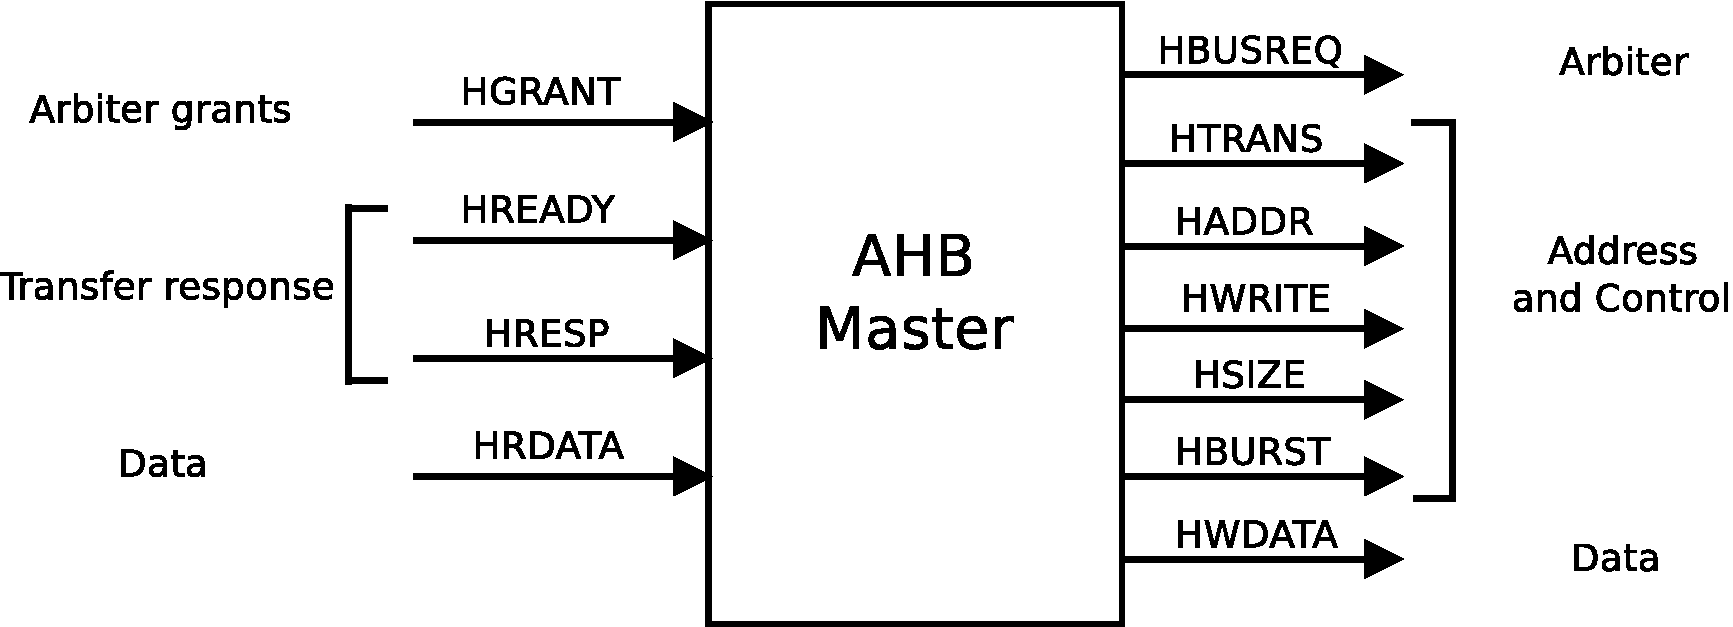
\includegraphics[width=0.7\textwidth]{figures/pdf/ahb_master_new.pdf}
    \caption{AHB master interface, with control and data signals. The HBUSSREQ and HGRANT signals  will be used take control over the bus.}
    \label{fig:masterint}
\end{figure}

 An AHB bus master has the most complex bus interface in an \amba~ system, and these interfaces are depicted in Figure \ref{fig:masterint}. The master contains one direct interface with the arbiter to receive and request the bus grant, a group of control signals to control the flow and duration of the transfer and to interfaces for reading and write data.  Typically an \amba~ system designer would use predesigned bus masters and therefore would not need to be concerned with the detail of the bus master interface.



\subsubsection{Slaves}

\begin{figure}[!ht]
    \centering
    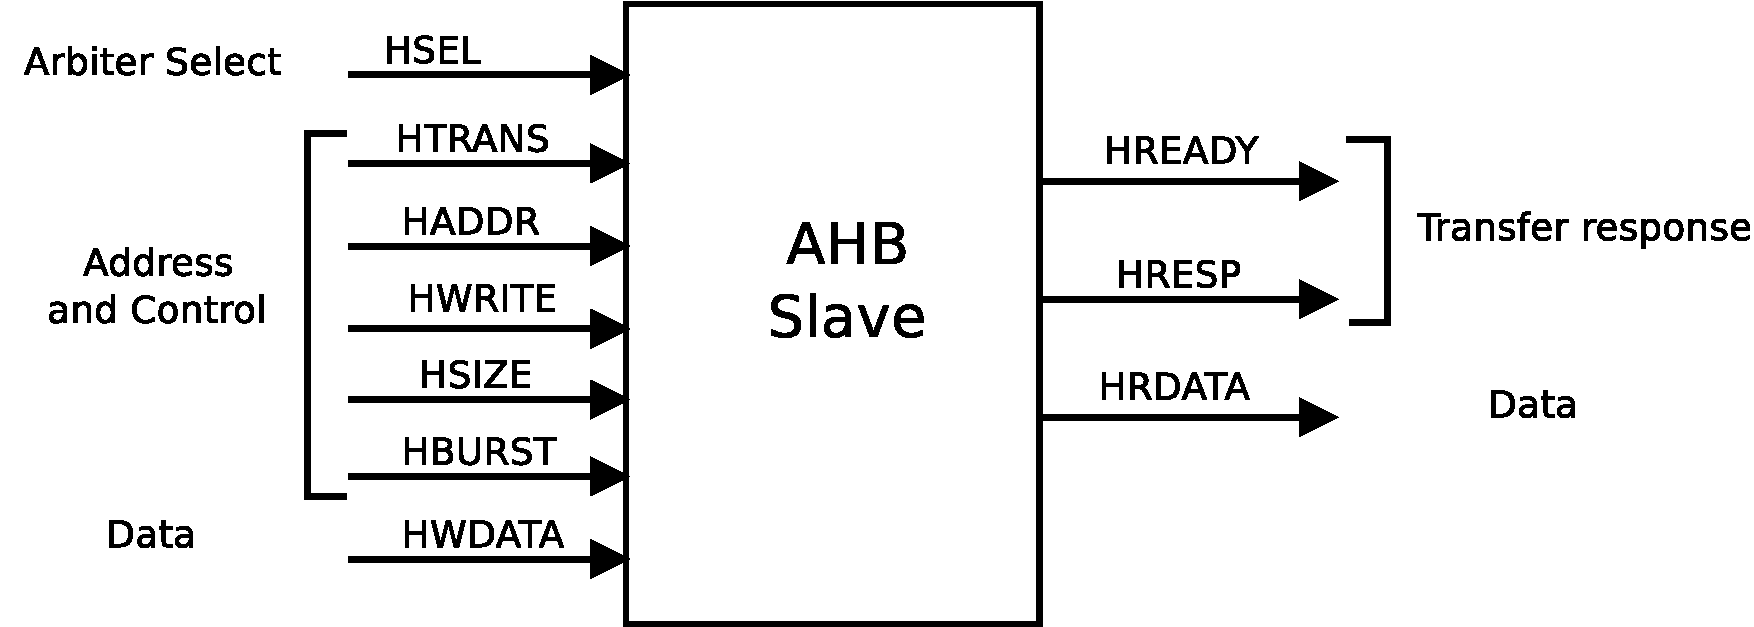
\includegraphics[width=0.7\textwidth]{figures/pdf/ahb_slave_new.pdf}
    \caption{AHB slave interface, where the HSEL signal will indicate when to start transfers.}
    \label{fig:slaveint}
\end{figure}
An AHB bus slave, as depicted in Figure \ref{fig:slaveint}, uses almost the same signals as the master, the difference is that the slave never controls the bus, so,  the interface with the arbiter is being selected as active and respond to transfers initiated by bus masters within the system. The slave uses an HSEL select signal from the decoder to determine when it should respond to a bus transfer. All other signals required for the transfer, such as the address and control information, will be generated by the bus master.
 
\subsubsection{Arbiter}
\begin{figure}[ht]
    \centering
    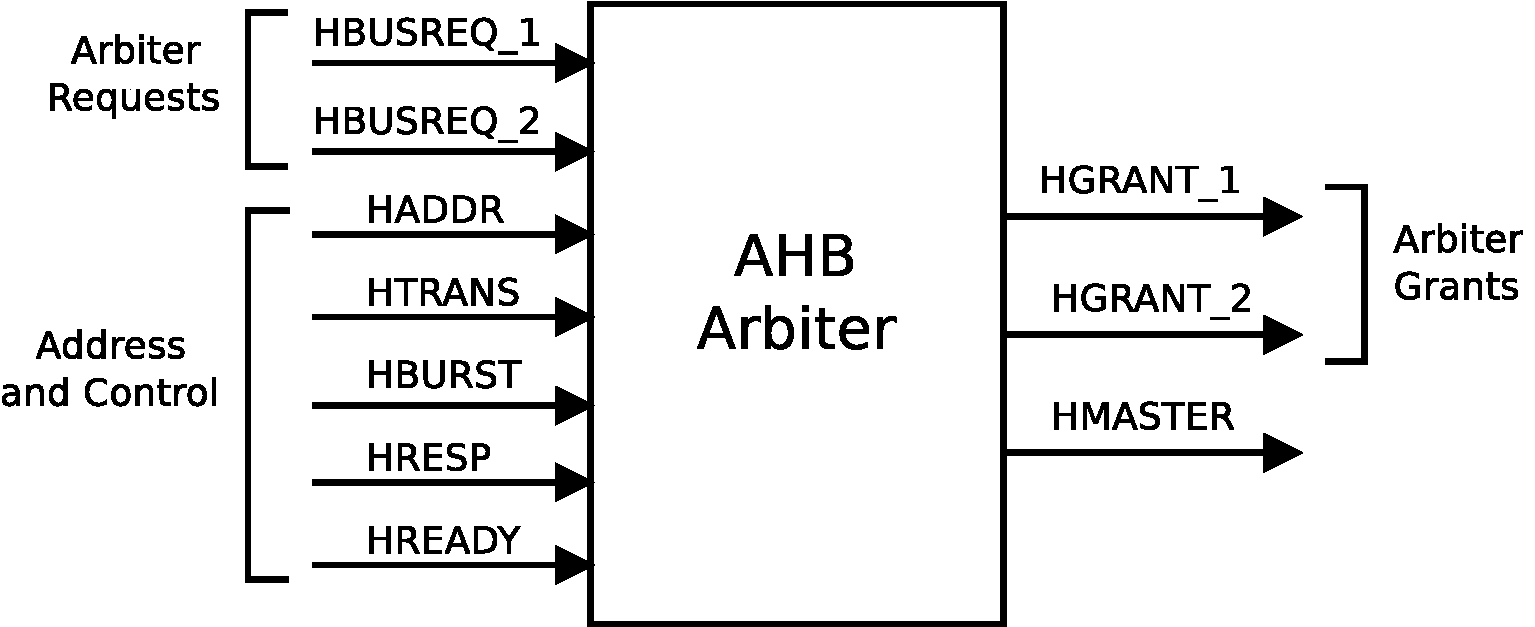
\includegraphics[width=0.7\textwidth]{figures/pdf/ahb_arbiter_new.pdf}
    \caption{AHB arbiter interface with one HGRANT and one HBUSSREQ for each master.}
    \label{fig:arbiterint}
\end{figure}

 The role of the arbiter in an \amba~ system is to control which master has access to the bus. As can be seen in Figure \ref{fig:arbiterint} every bus master has a REQUEST / GRANT interface to the arbiter and the arbiter uses a prioritization scheme to decide which bus master is currently the highest priority master requesting the bus. The detail of the priority scheme is not specified and is defined for each application. It is acceptable for the arbiter to use other signals, either \amba~ or non-\amba~, to influence the priority scheme that is in use.
 The address and control signals are used by the arbiter to route the HWDATA and the HADDR from the granted master to the selected slave as illustrated in Figure     \ref{fig:internorg}.
 
 
 \subsubsection{Arbitration}
 
 The arbitration process needs specific control signals, despite the ones described below, two more signals are used in the \amba~ system, HLOCK and HSPLIT,  the first to indicate that the master wants exclusive access to the bus, the second to restart transactions when they are interrupted.
 
 \begin{itemize}

\item  {HBUSREQ - } The bus request signal is used by a bus master to request access to the bus. Each bus master has an HBUSREQ signal to the arbiter and there can be up to 16 separate bus masters in any system.

%\item  {\textbf{HLOCKx -}} A master asserts the lock signal at the same time as the bus request signal. This indicates to the arbiter that the master is performing many indivisible transfers and the arbiter must not grant any other bus master access to the bus once the first transfer of the locked transfers has commenced. HLOCKx must be asserted at least a cycle before the address to which it refers, in order to prevent the arbiter from changing the grant signals.

\item  {HGRANT - } The grant signal is generated by the arbiter and indicates that the appropriate master is currently the highest priority master requesting the bus, taking into account locked transfers and SPLIT transfers. A master gains ownership of the address bus when HGRANT is HIGH and HREADY is HIGH at the rising edge of HCLK.

\item  {HMASTER - } The arbiter indicates which master is currently granted using the HMASTER signal and,  this same signal can be used to control the central address and control multiplexer, automatically routing the correct HDATA and control signals to the correct slave. The master number is also required by SPLIT-capable slaves so that they can indicate to the arbiter which master can complete a SPLIT transaction.

%\item  {\textbf{HMASTLOCK -}} The arbiter indicates that the current transfer is part of a locked sequence by asserting the HMASTLOCK signal, which has the same timing as the address and control signals.

%\item  {\textbf{HSPLIT[15:0] -}} The 16-bit Split Complete bus is used by a SPLIT-capable slave to indicate which bus master can complete a SPLIT transaction. This information is needed by the arbiter so that it can grant the master access to the bus to complete the transfer.
\end{itemize}

An Example of a master requesting the bus control is shown in Figure \ref{fig:gnwsm} where the arbiter grants the access after a few waiting cycles.
%  \begin{figure}[ht]
%     \centering
%     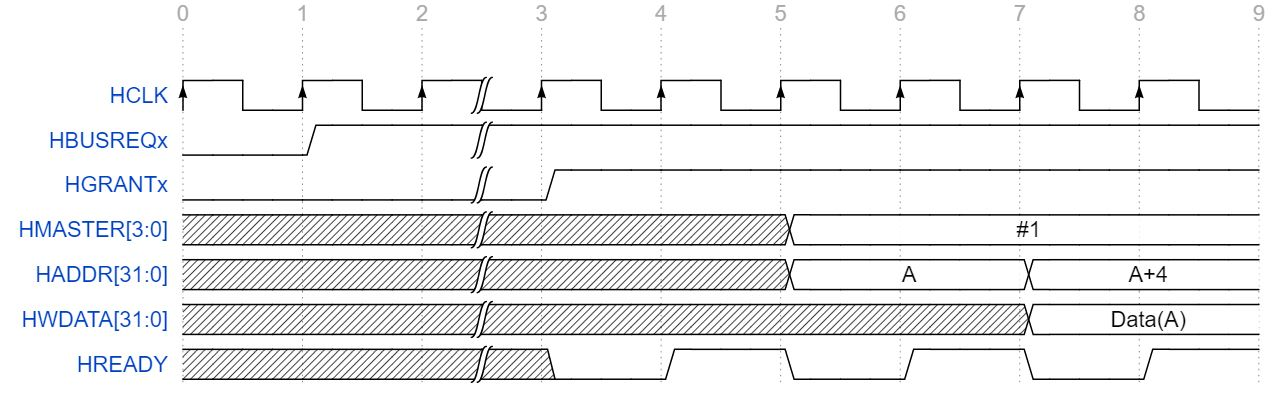
\includegraphics[width=\textwidth]{figures/read_grant_wc_new.JPG}
%     \caption{Granting with wait cycles}
%     \label{fig:grantwait}
% \end{figure}


\subsubsection{Decoder}

\begin{figure}[ht]
    \centering
    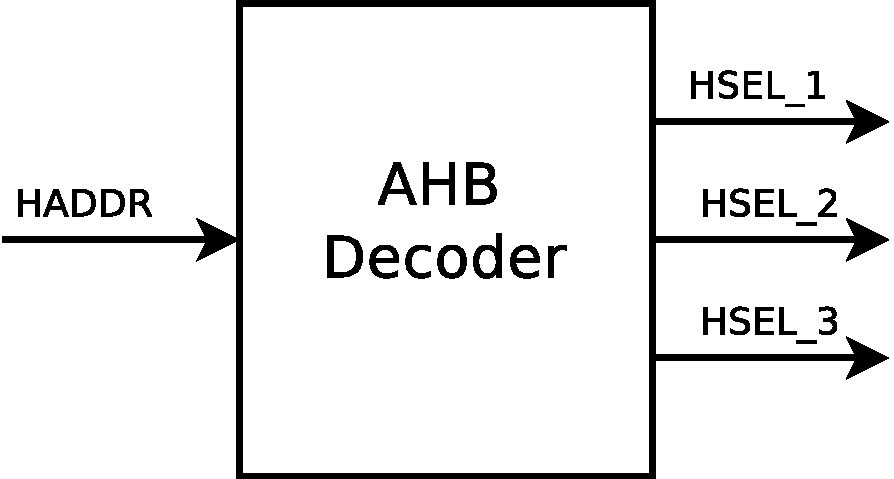
\includegraphics[width=0.6\textwidth]{figures/pdf/ahb_decoder_new.pdf}
    \caption{AHB Decoder interface}
    \label{fig:decoder int}
\end{figure}
 The decoder in an \amba~ system is used to perform a centralized address decoding function, which improves the portability of peripherals, by making them independent of the system memory map. The Idea is that the decoder will snoop the address and select with slave will respond to the transaction, also, as shown in figure \ref{fig:internorg} the decoder will indirectly control a demultiplexer that will route the signals from the correct slave to the granted master.

 

\section{\cshia~Components}
\label{sec:Components-of-the-Architecture}
\mario{Try a top down approach}
As Section \ref{subsec:integrity} discussed, the main resource to provide integrity are tags. Since \cshia~uses \puf-based keys to generate tags, we called them \puf-Tags, or \ptags~for short. \ptags~are the core of \cshia's design. They will be unique for each instance of \cshia~due to the unclonability property of \pufs. That ensures a one-to-one relationship between programs and instances, providing authenticity. To handle \ptags, three main components are added to conventional embedded system architecture. They are: The \ptag~Memory; the Bus Handler (\handler); and the Security Engine (\seceng). Figure \ref{fig:cshia} shows this design and how components communicate between themselves. 

\ptag~Memory is an external memory and has its own buses. This architectural decision gives freedom to designers that can choose bus width, frequency, address space, etc. Because the processor is not aware of any additional component of \cshia, \handler~intercepts data transfers between processor and memory in order to provide them to \seceng~that generates tags. \handler~can also request data ( on behalf of the processor) to main memory so as form complete memory blocks that are necessary to generate \ptags.

\seceng~has three major sub-components. The main one is the \ptag~Generator (\ptaggen), which uses input data whose length is equal to a memory block concatenated with its address to generate \ptags. The \fuzzy~is only used when the system loses its secret key, for instance, after a power cycle. Thus, when the system is powered on, the \fuzzy~will extract the \puf-based key and provide it to \ptaggen. Finally, we have the \ptag~Memory Management Unit (\pmmu). The main functions of the \pmmu~are to store and request \ptags~from the \ptagmem~and also to decode internal addresses of \ptags~to physical addresses of \ptagmem. 


%======================================================
%Bus Handler
%======================================================
\subsection{Bus Handler (\handler)}
\label{subsec:bushandler}
To implement the \cshia~ architecture, all the security operations described in \ref{sec:opmodes} will be performed using a set of words, ideally an entire cache line that the processor might request but that can be multiple cache lines or any other combination necessary to be in the format of the \seceng~ input, this set of words required to calculate the \ptags~ from now on will be referred as \sline.  The \handler~ has three main functions, monitoring the processor request and respond it when necessary, assemble a \sline~  and prevent the processor the execute unsafe or unverified instructions  as well as don't let  it  write in the bus any unsafe operation. In this context any instruction or data requested written by the processor that was not verified by the \seceng~ is considered unsafe.



%======================================================
%Block Diagram
%======================================================
\subsubsection{Block Diagram}

\begin{figure*}[!ht]
    \centering
    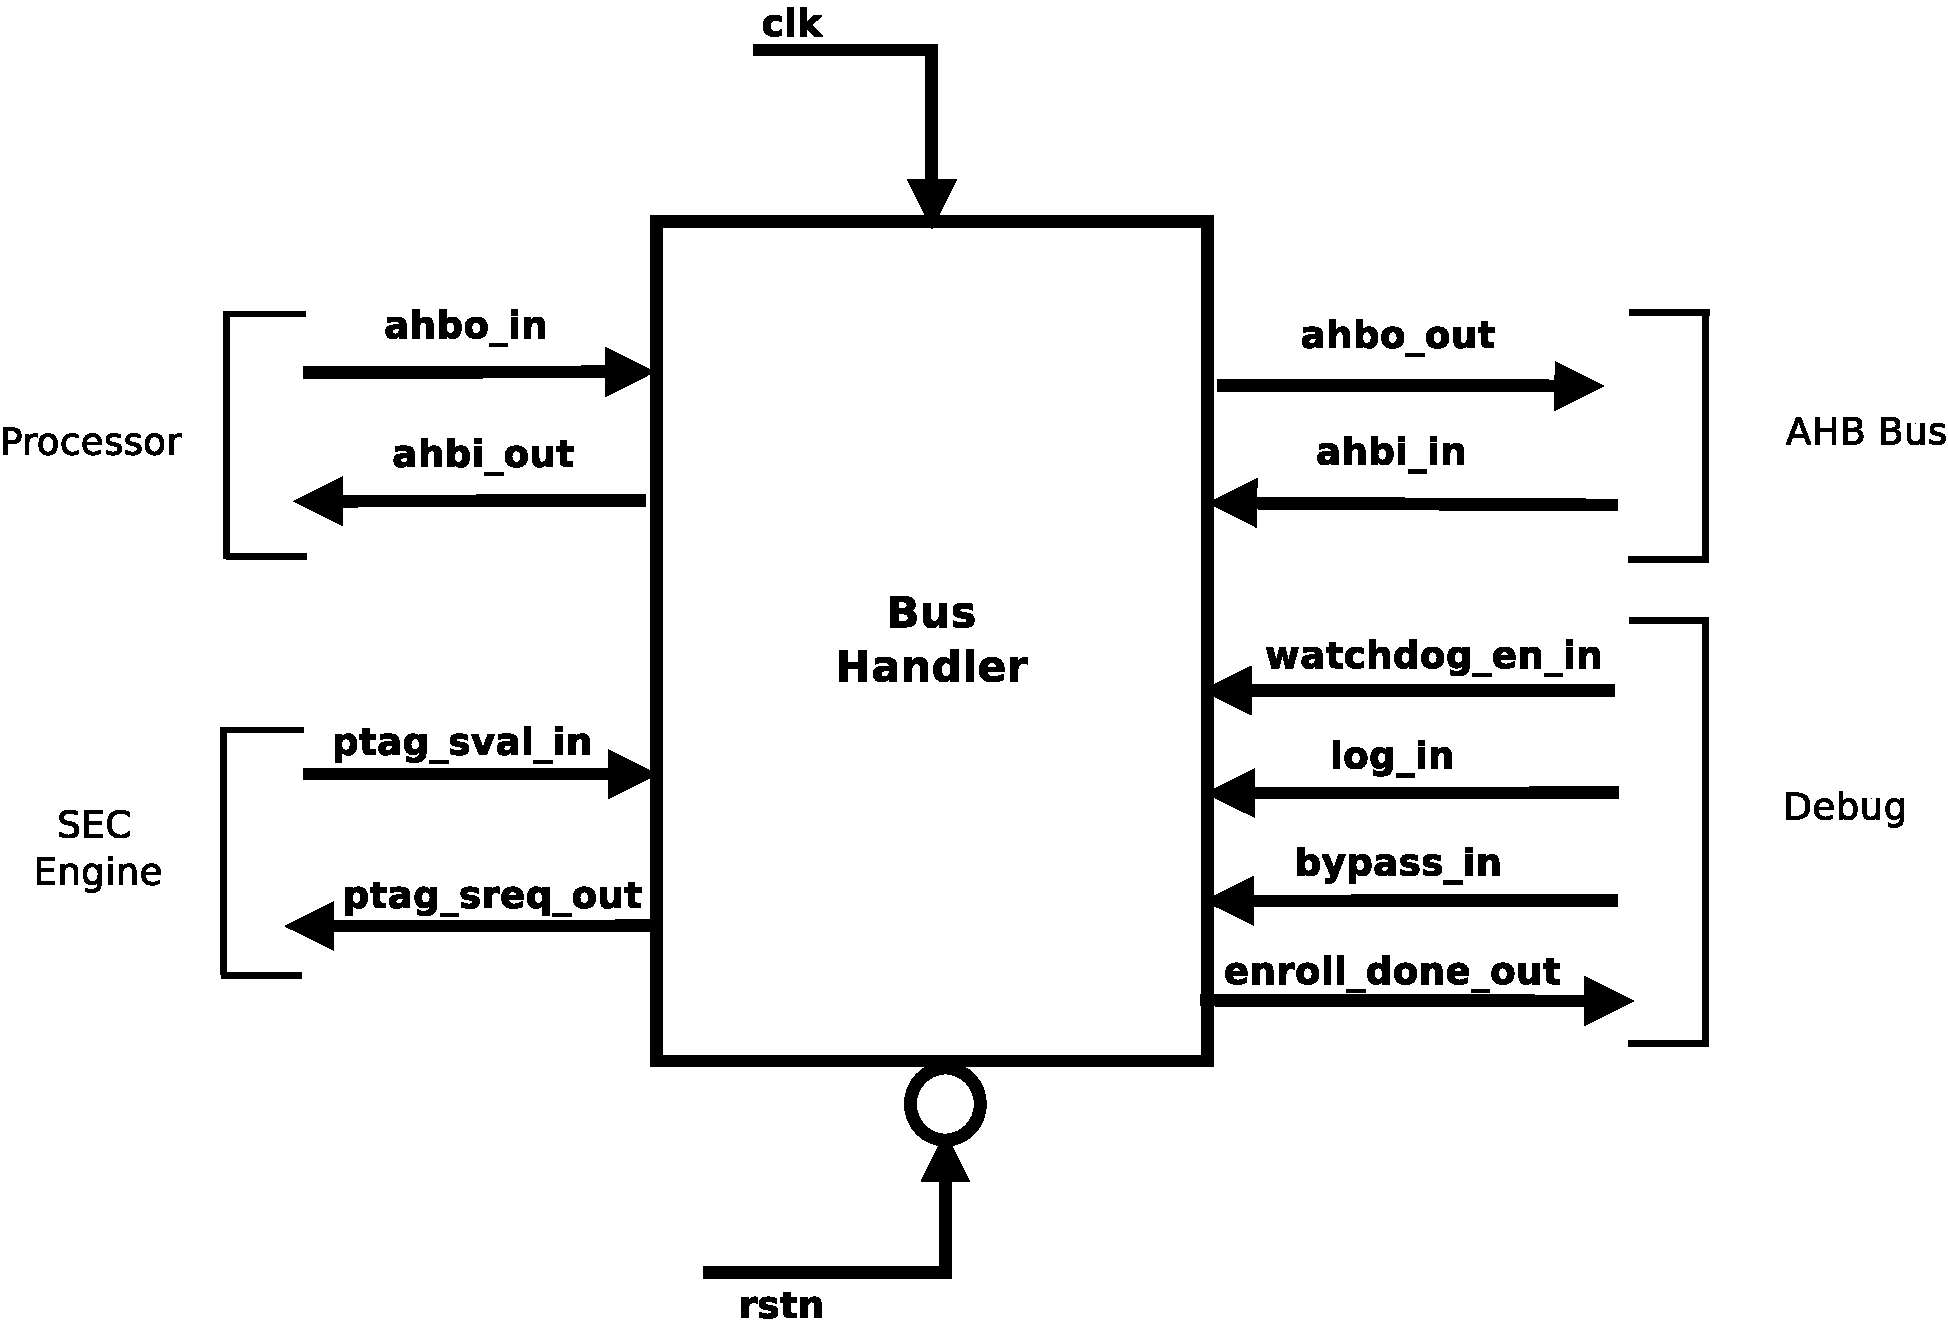
\includegraphics[scale=0.35]{bus_handler}
    \caption{Bus Handler  interface }
%    \vspace*{-9pt} 
    \label{fig:bhbb}
\end{figure*}


%======================================================
%Signal Description
%======================================================
\subsubsection{Signal Description}

The inputs and outputs of this block can be split in four interfaces,
the signals  ahbo\_in and ahbi\_out the interface with the processor,  ahbo\_out  and ahbi\_in
the interface with the bus, ptag\_sval\_in and ptag\_sreq\_out with the security engine and control and debug signals as described in Table \ref{table:shports}.
 The description of each type can be found in Appendix \ref{ap:signals}.

\begin{table}[H]
% \centering
\begin{tabular}{l l l l}
\textbf{Port}   & \textbf{in/out} & \textbf{Type}        & \textbf{Description} 	\\ \hline \hline
clk             & in              & std\_ulogic          & system clock         	\\ \hline
rstn            & in              & std\_logic           & negated rset         	\\ \hline
ptag\_sreq\_out & out             & ptag\_sec\_req\_type & security check request    	\\ \hline
ptag\_sval\_in  & in              & ptag\_sec\_val\_type & security check response  	\\ \hline
ahbi\_in        & in              & ahb\_mst\_in\_type   & AHB input from bus      	\\ \hline
ahbi\_out       & out             & ahb\_mst\_in\_type   & AHB output to processor      \\ \hline
ahbo\_in        & in              & ahb\_mst\_out\_type  & AHB input from processor    \\ \hline
ahbo\_out       & out             & ahb\_mst\_out\_type  & AHB output to BUS            \\ \hline
std\_logic         
bypass\_in      & out             & std\_logic           & bypass input         	\\ \hline
log\_in         & in              & std\_logic           & log bus activities       \\ \hline
watchdog\_en\_in  & in            & std\_logic           & enable a watchdog             \\ \hline
enroll\_done     & out             & std\_logic          & enrollment phase status            \\ \hline

\end{tabular}
 \caption{Description of the \handler~ ports .}
 \label{table:shports}

\end{table}

\subsubsection{Functional Description}

\begin{figure*}[!ht]
	\centering
	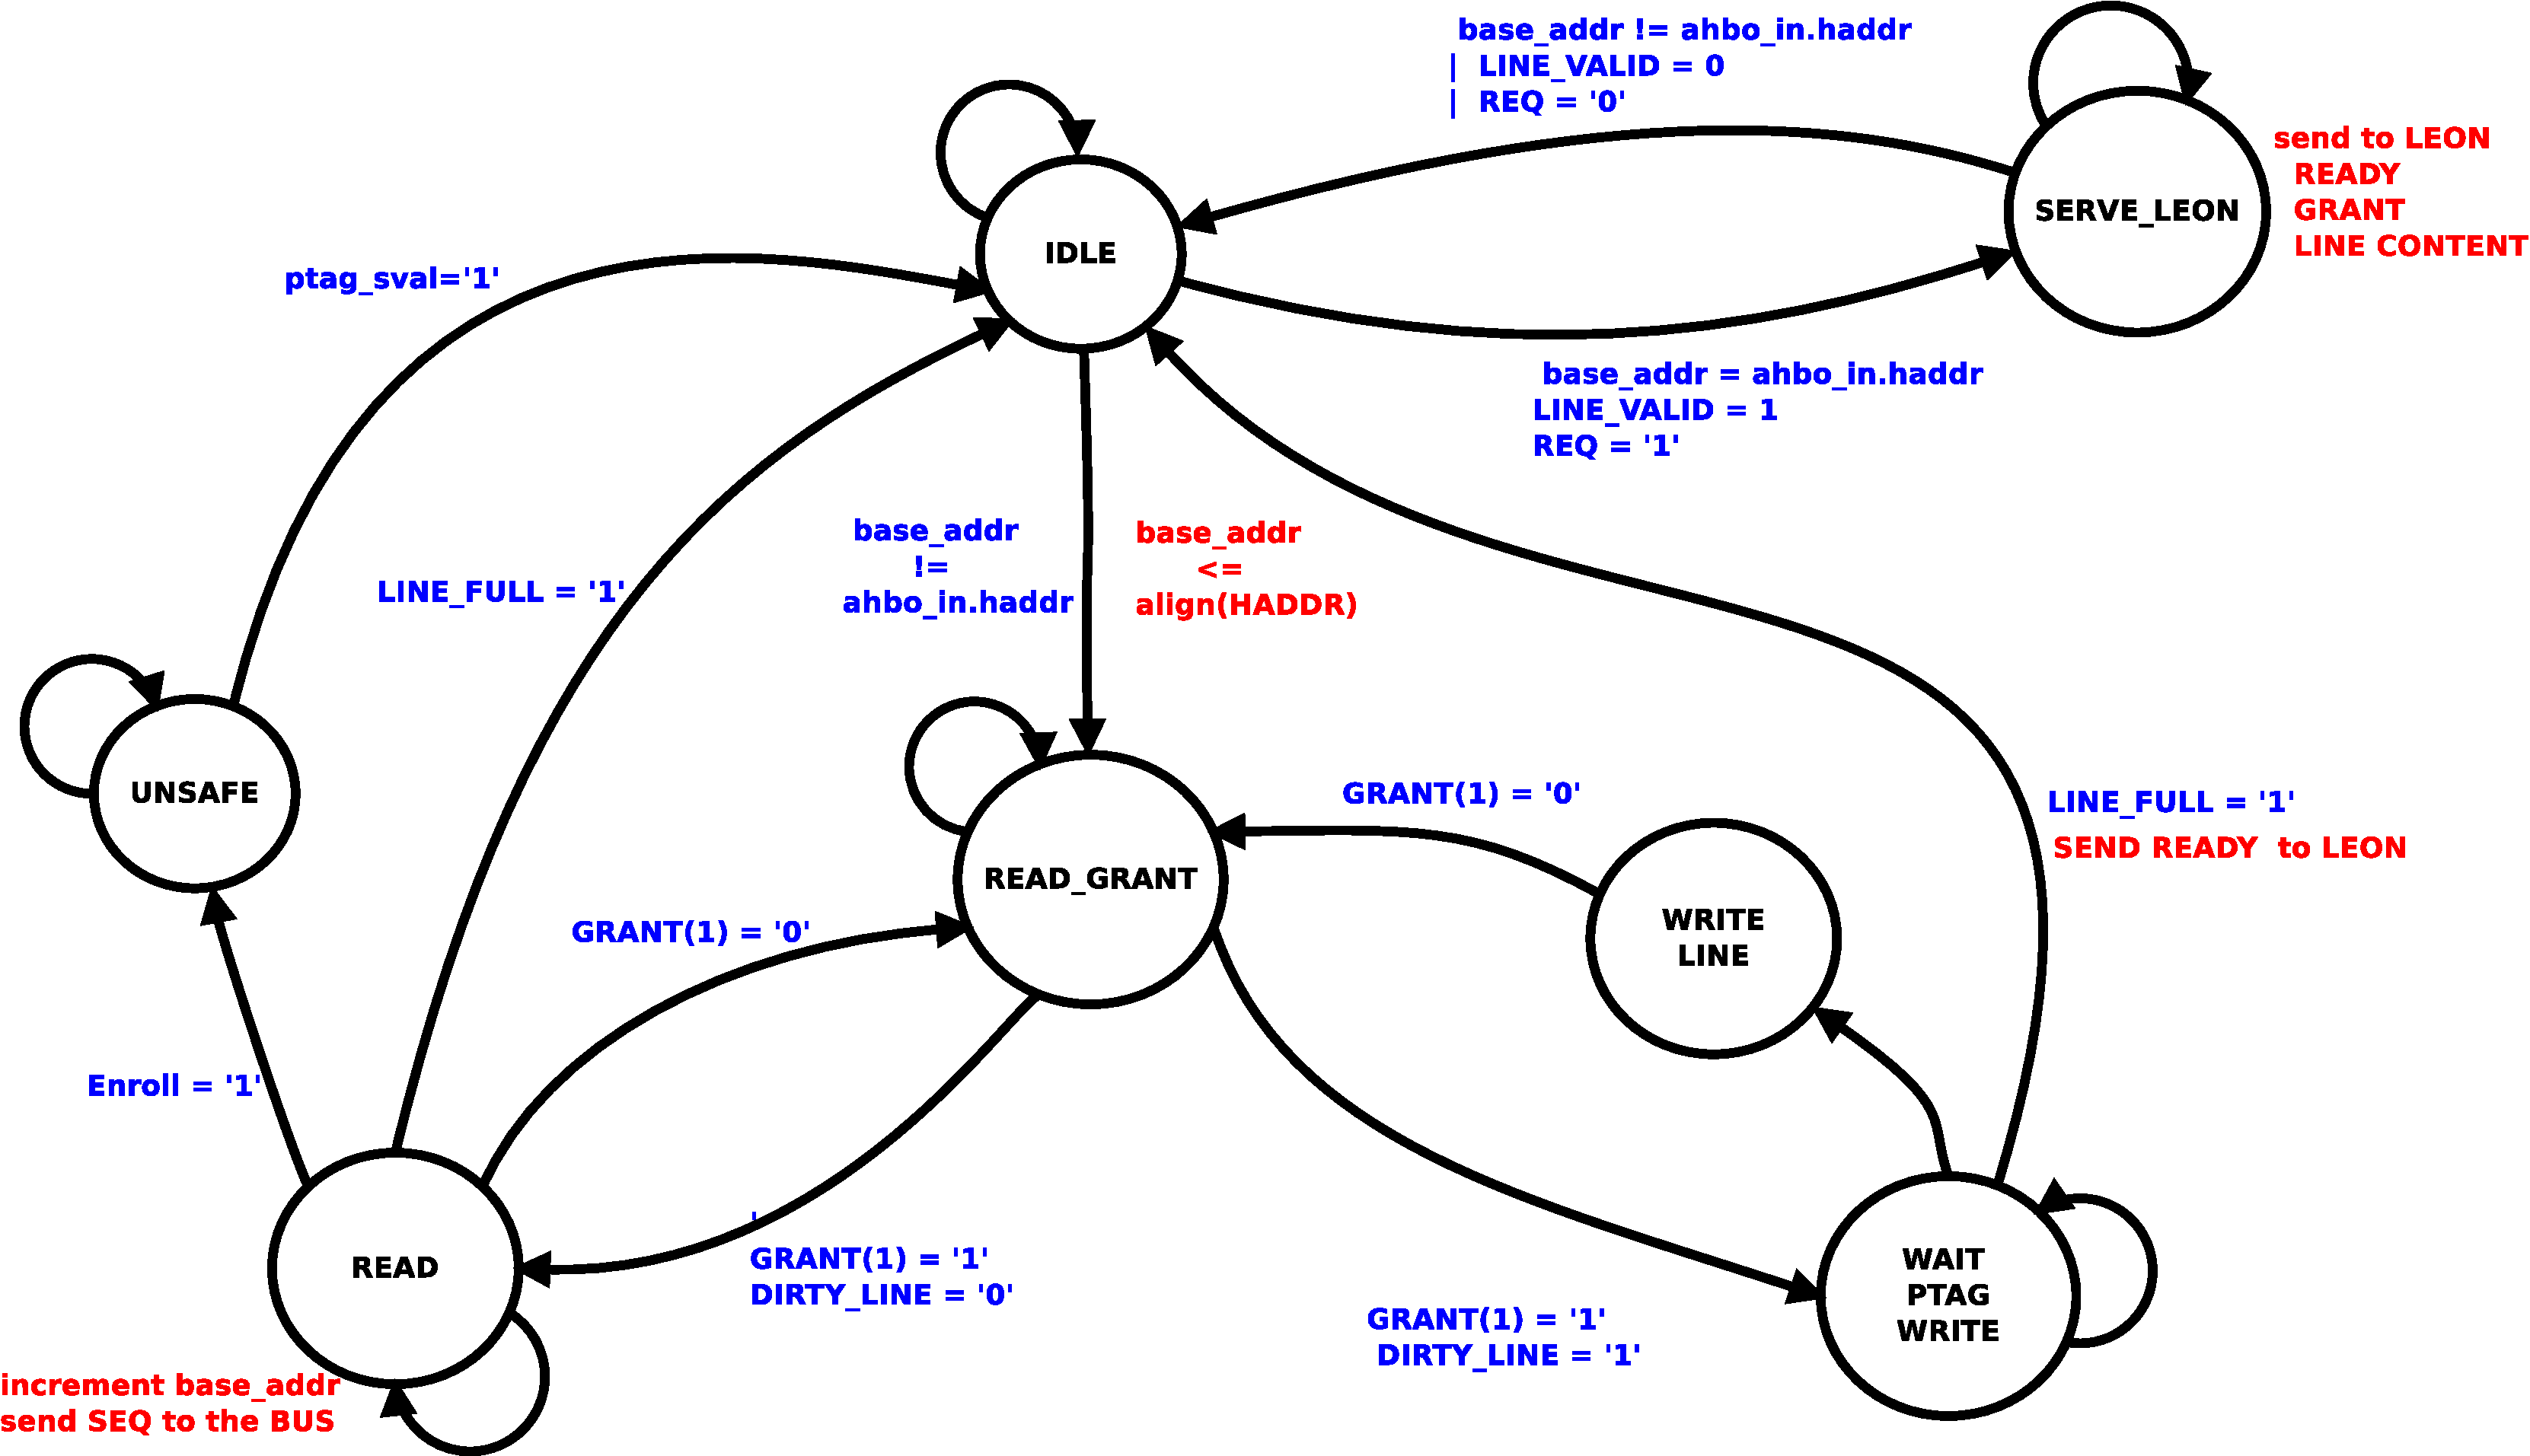
\includegraphics[scale=0.25]{figures/pdf/sec_hand_state_machine.pdf}
    \caption{Bus Handler state machine. The blue text indicate the condition necessary to the transition to happen, the red text indicates the \handler~ actions.   }
%	\vspace*{-9pt} 
	\label{fig:phsm}
\end{figure*}

As shown in Figure \ref{fig:cshia} the processor will see the \handler~ as the bus, and by the bus as the processor, assembling \slines~  and constantly sending those lines to \seceng.  To store the \slines, an internal buffer with a configurable size is used; this is the \handler~ \sline~ buffer and will be from now on referred to as \sbuf.  When the processor requests the bus, the \handler  will assert the grant, and depending on the state of the \sbuf, load new \slines~ from the bus or send one from the \sbuf. The \handler~ is implemented using a state machine which gives the block stability to assemble the \sline~ and to control the flow to the processor and to \seceng. Since this state machine controls all \handler~ operations the functional  description of this block can be explained using the state transitions  of Figure \ref{fig:phsm} and the following state description:

\begin{itemize}
 \item{\textbf{IDLE}}
 
The system stays in this state until the processor asserts HBUSSREQ, at this time the \handler~, on behalf of the arbiter, will answer these requests according to one of these scenarios:
 \begin{enumerate}
     \item The \sbuf~ contains the address requested by the processor in a \sline~ - In this case, the processor can start the transaction in the SERVE LEON state.
     \item The address requested is not in the \sbuf~ - In this scenario, the \handler~ will get the grant in the READ GRANT state and evaluate if its a read or a write, then assemble a new \sline.
     \item The processor requested a line that was not verified or verified incorrectly by \seceng~ -  In this case, the system will halt because a security flaw was detected.
 \end{enumerate}

 
  \item{\textbf{READ GRANT}}

  This state is required for any transaction in the bus, it requests the bus grant for the arbiter, asserting the HBUSSREQ signal on behalf of the processor before beginning the transaction. The arbiter can answer in two possible ways, with or without wait states, for the first, illustrated in Figure \ref{fig:gnwsm},  the HBUSSREQ is asserted in time $2$, by the time the arbiter responds, at time $3$, HGRANT and HREADY are asserted  indicating that the transaction can start in the next cycle. For the second, depicted in figure \ref{fig:gwsm}, The  HBUSSREQ is asserted on time $2$, but the HREADY signal is only asserted on time $5$ delaying the start of the transactions to time $7$, in situations like this the HREADY signal regulates all the traffic. 
  
  
\begin{figure}[!ht]
    \centering
    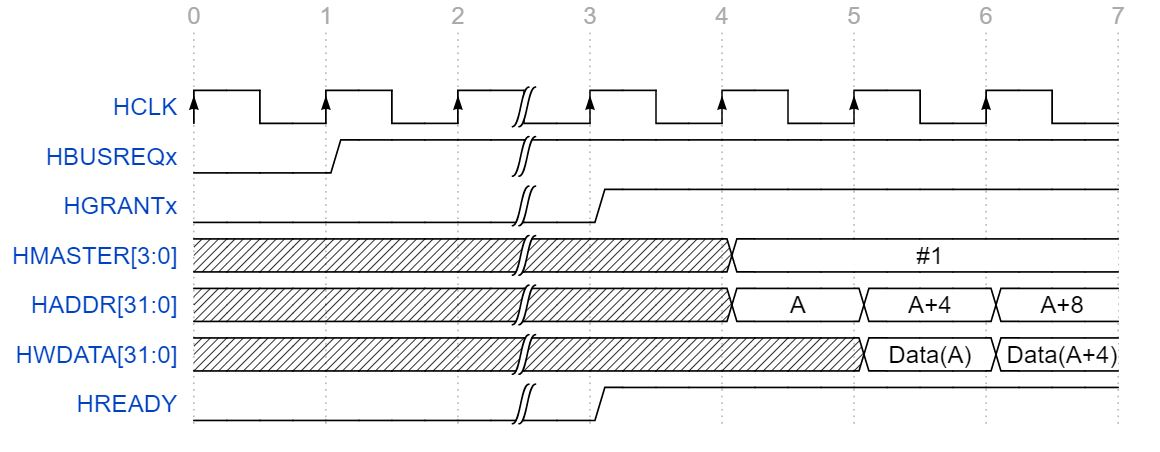
\includegraphics[width=\textwidth]{figures/others/read_grant_no_wait_new.JPG}
    \caption{Requesting grant with no wait states  }
    \label{fig:gnwsm}
\end{figure}


\begin{figure}[!ht]
    \centering
    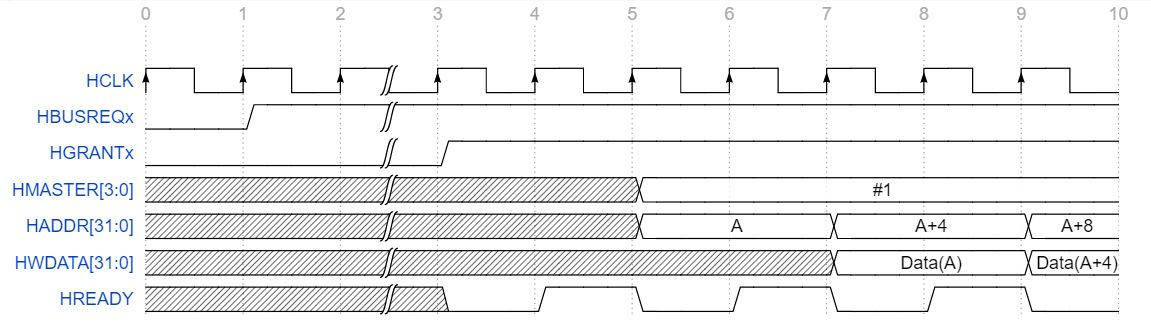
\includegraphics[width=\textwidth]{figures/others/read_grant_ec_new_exended.JPG}
    \caption{Requesting grant with wait states  }
    \label{fig:gwsm}
\end{figure}

  
  Once the arbiter asserts HGRANT,  the \sbuf~ is checked, and one of the positions is selected to be replaced, if the chosen \sline~ contains any updated value by the processor, then it needs to be written in the memory before loading a new \sline. In this is the case, \handler~ will send it to the \seceng~ to calculate a new \ptag~ before writing the line in the memory,  then change to WAIT PTAG WRITE  state while the security operations are done. If no changes were made in the \sline then a new one is loaded in the READ LINE state. 
  
  \item{\textbf{READ LINE}}
  
  A new \sline will be loaded from the main memory into the \sbuf to start a transaction after the bus is granted and all the control signals are in place, as described in section \ref{sec:amba2}. The Figure \ref{fig:ublsm} illustrates two different incremental read transfers,  the first  starts on time $2$ indicated by the first HTRANS=NONSEQ, with  halfword size reading positions $0$x$20$ and $0$x$22$, the second transaction starts at time $4$ where a small delay is exemplified to show how the HREADY controls the bus operations, and then three words are transferred to the master.  Once an entire \sline is transferred, the line is sent to \seceng~ and the state is set to IDLE again, where the system will halt until the execution is considered secure.
  After a power cycle, all the instructions are read and tagged, in this case, the execution is not safe, so the state is set to UNSAFE before going back to IDLE. This process is explained in Section \ref{sec:opmodes}.

  
 
  \begin{figure}[!ht]
    \centering
    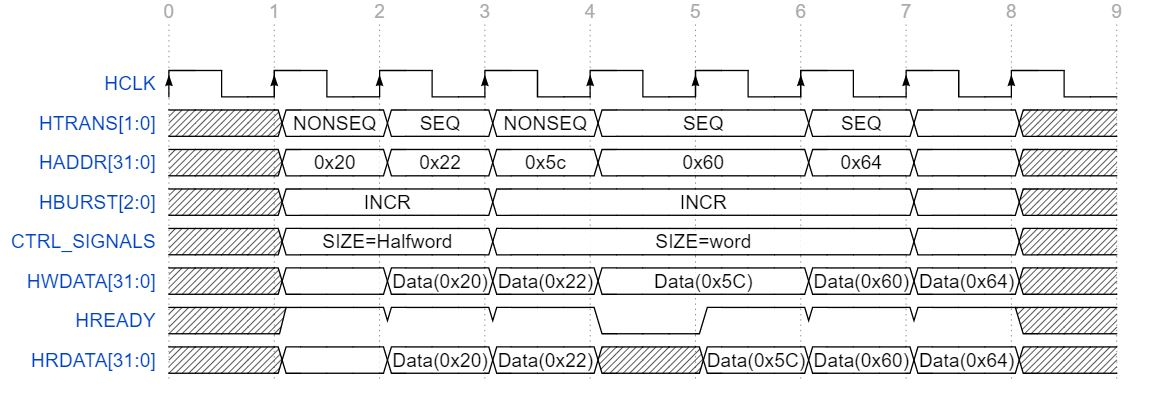
\includegraphics[width=\textwidth]{figures/others/basic_transfer_w_ctrl_new.JPG}
    \caption{Incremental burst transfers with halfword and word.}
    \label{fig:ublsm}
  \end{figure}
  
 \item{\textbf{WAIT PTAG WRITE}}
 When a \sline need to be written, first is sent to the \seceng~ to calculate the respective \ptag~ and store in the \ptagmem, this process can take a different number of cycles depending on the features used in the \seceng~, this process is explained in Section \ref{sec:secengine}. After the \ptag is calculated the line can be written in the state WRITE LINE.
 
 
 \item{\textbf{WRITE LINE}}
   \begin{figure}[H]
    \centering
    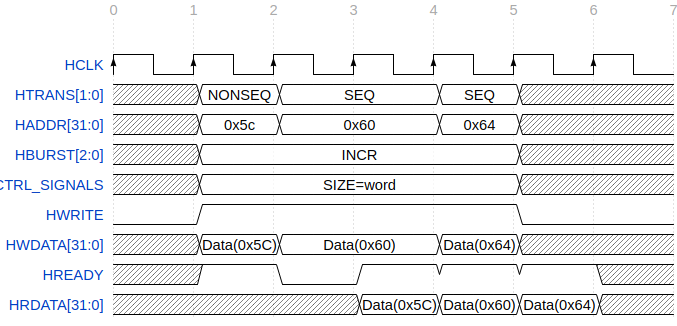
\includegraphics[width=\textwidth]{figures/others/ahbwrite.png}
    \caption{Incremental write burst of words.}
    \label{fig:ahbwrite}
  \end{figure}
The write process is much similar to the read, as Figure \ref{fig:ahbwrite} shows the difference is the HWRITE signal that is asserted during the entire transfer. After the write is completed the state is set to IDLE and the \handler~ is ready to send respond the processor requests.

 \item{\textbf{SERVE LEON}}

 On this state all LEON requests read or write are executed, the \handler~~will assert the HGRANT and starting acting like the bus until there is data in the \sbuf. The transfers towards the processor are the same as described before in Figures \ref{fig:ublsm} and \ref{fig:ahbwrite}, when the processor requests any address that is not on the \sbuf, the state is set to IDLE.
 
\item{\textbf{UNSAFE}}
After a power cycle all the instructions are read and tagged in a process called enrollment that can take a different number of cycles depending on the features used in the \seceng~, the enrollment is explained in Section \ref{sec:opmodes}. After a \sline is considered secure during the enrollment phase, the state goes to IDLE.
 
\end{itemize}

%======================================================
%Security Engine
%======================================================
\subsection{Security Engine}
\label{sec:secengine}

\begin{figure*}[!ht]
    \centering
    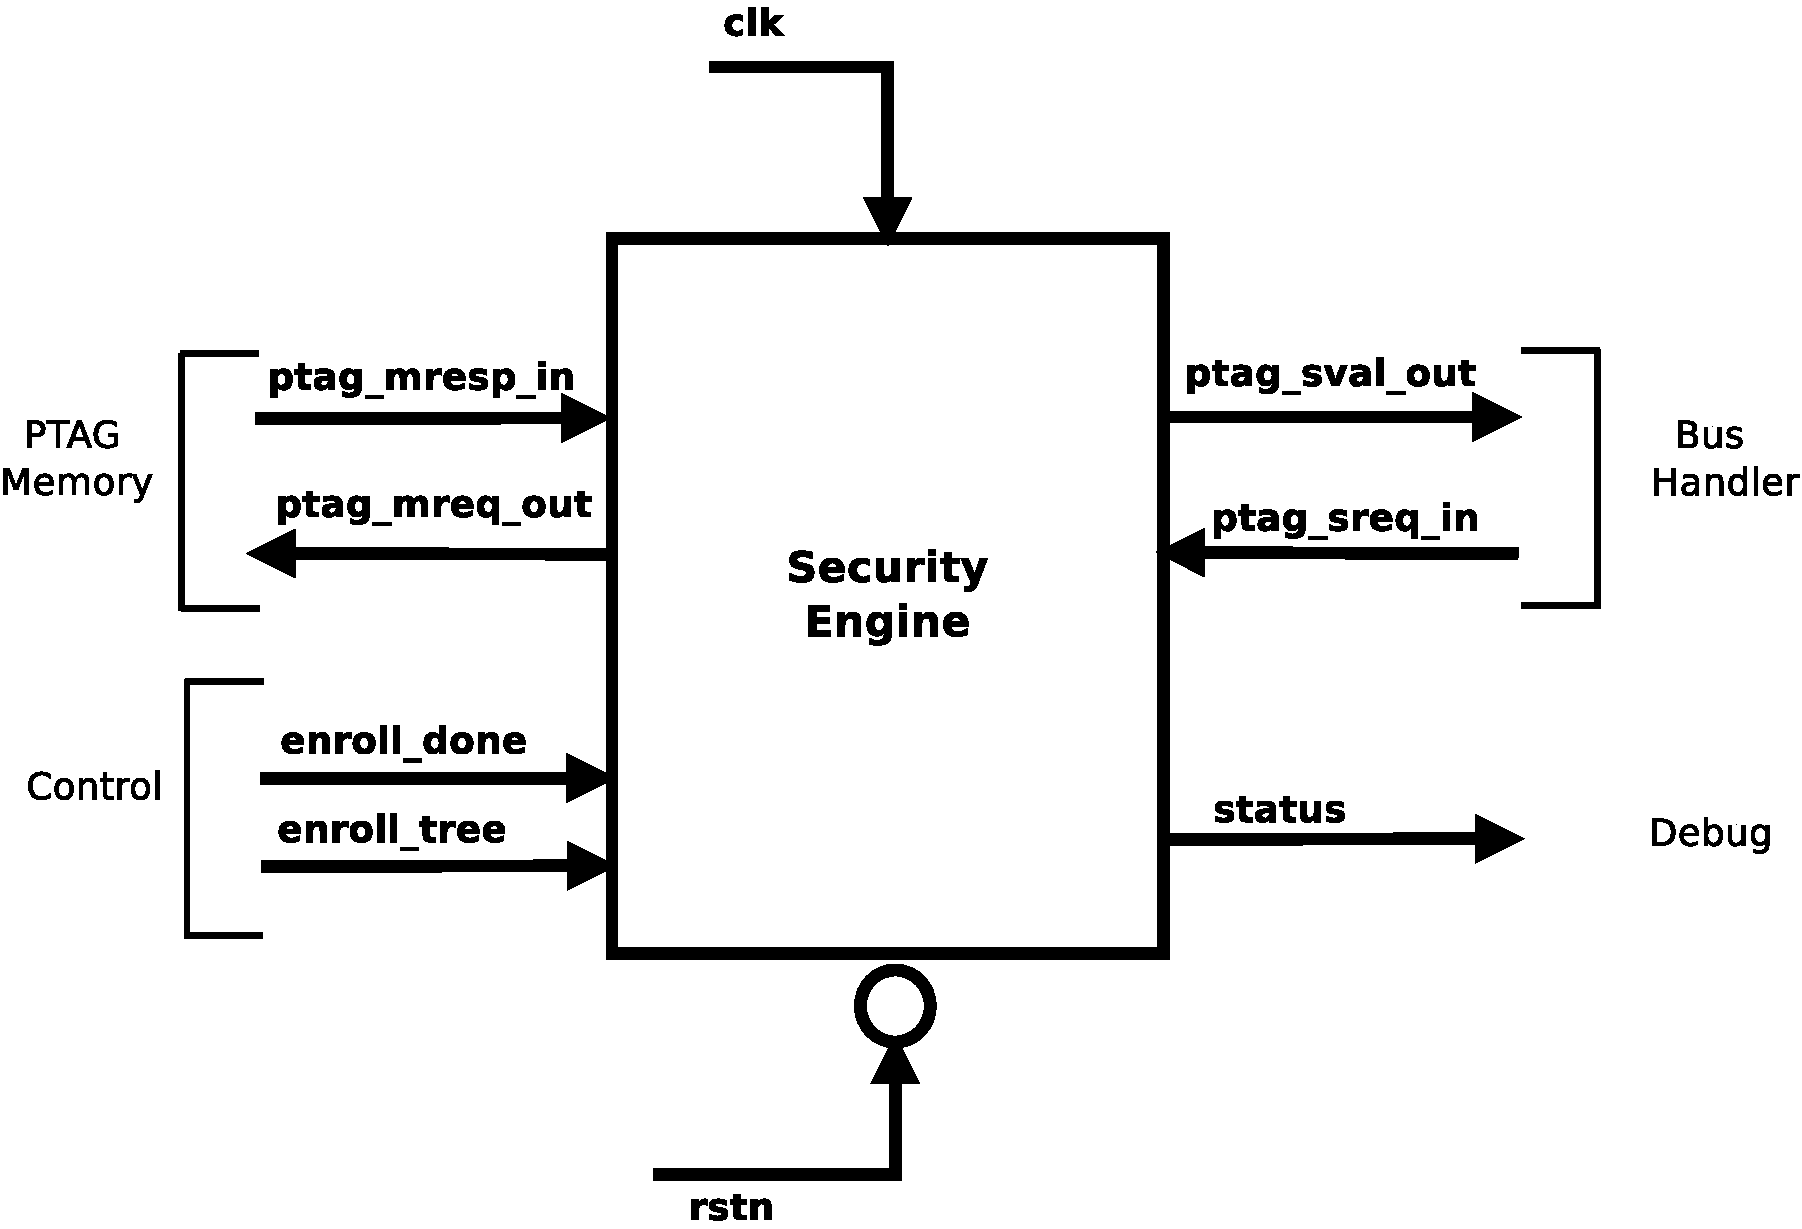
\includegraphics[scale=0.35]{security_engine_bb}
    \caption{Security engine interface.  }
%    \vspace*{-9pt} 
    \label{fig:sebb}
\end{figure*}


This block is responsible for the security part of \cshia~,  as shown in Figure \ref{fig:sebb} it contains one interface toward the \ptagmem~ to read and write \ptags~, one interface towards the \handler~  and also control and debug signals described in Table \ref{table:seports}.  The \seceng~ has three main functions, extract the key from the \puf~, generate and validate \ptags~ and make the \ptagmem operations transparent to \handler~ and the processor.



\subsubsection{Signal Description}
%TODO remove the enroll tree
\begin{table}[H]
    \centering
    \begin{tabular}{l l l l}
    
        \textbf{Port}   & \textbf{in/out} & \textbf{Type}        & \textbf{Description} 	\\ \hline \hline
        clk             & in              & std\_ulogic          & system clock         	\\ \hline
        rstn            & in              & std\_logic           & negated reset         	\\ \hline
        ptag\_sreq\_in  & in              & ptag\_sec\_req\_type & security check request    	\\ \hline
        ptag\_sval\_out & out             & ptag\_sec\_val\_type & security check response  	\\ \hline
        ptag\_mreq\_out & out             & ptag\_mreq\_type 	 & ptag memory  request    	\\ \hline
        ptag\_mresp\_in & in              & ptag\_mresp\_type 	 & ptag memory  response  	\\ \hline
        enroll\_done    & in              &  std\_logic      	 & enroll phase status  	\\ \hline
        %enroll\_tree    & in              &  std\_logic      	 & \mt~control 	\\ \hline
        status          & in              &  std\_logic      	 & internal state 	\\ \hline
        
    \end{tabular}
    \caption{Description of the \seceng~ ports.}
    \label{table:seports}
\end{table}




\subsubsection{Functional Description}

\begin{figure}[!ht]
    \centering
    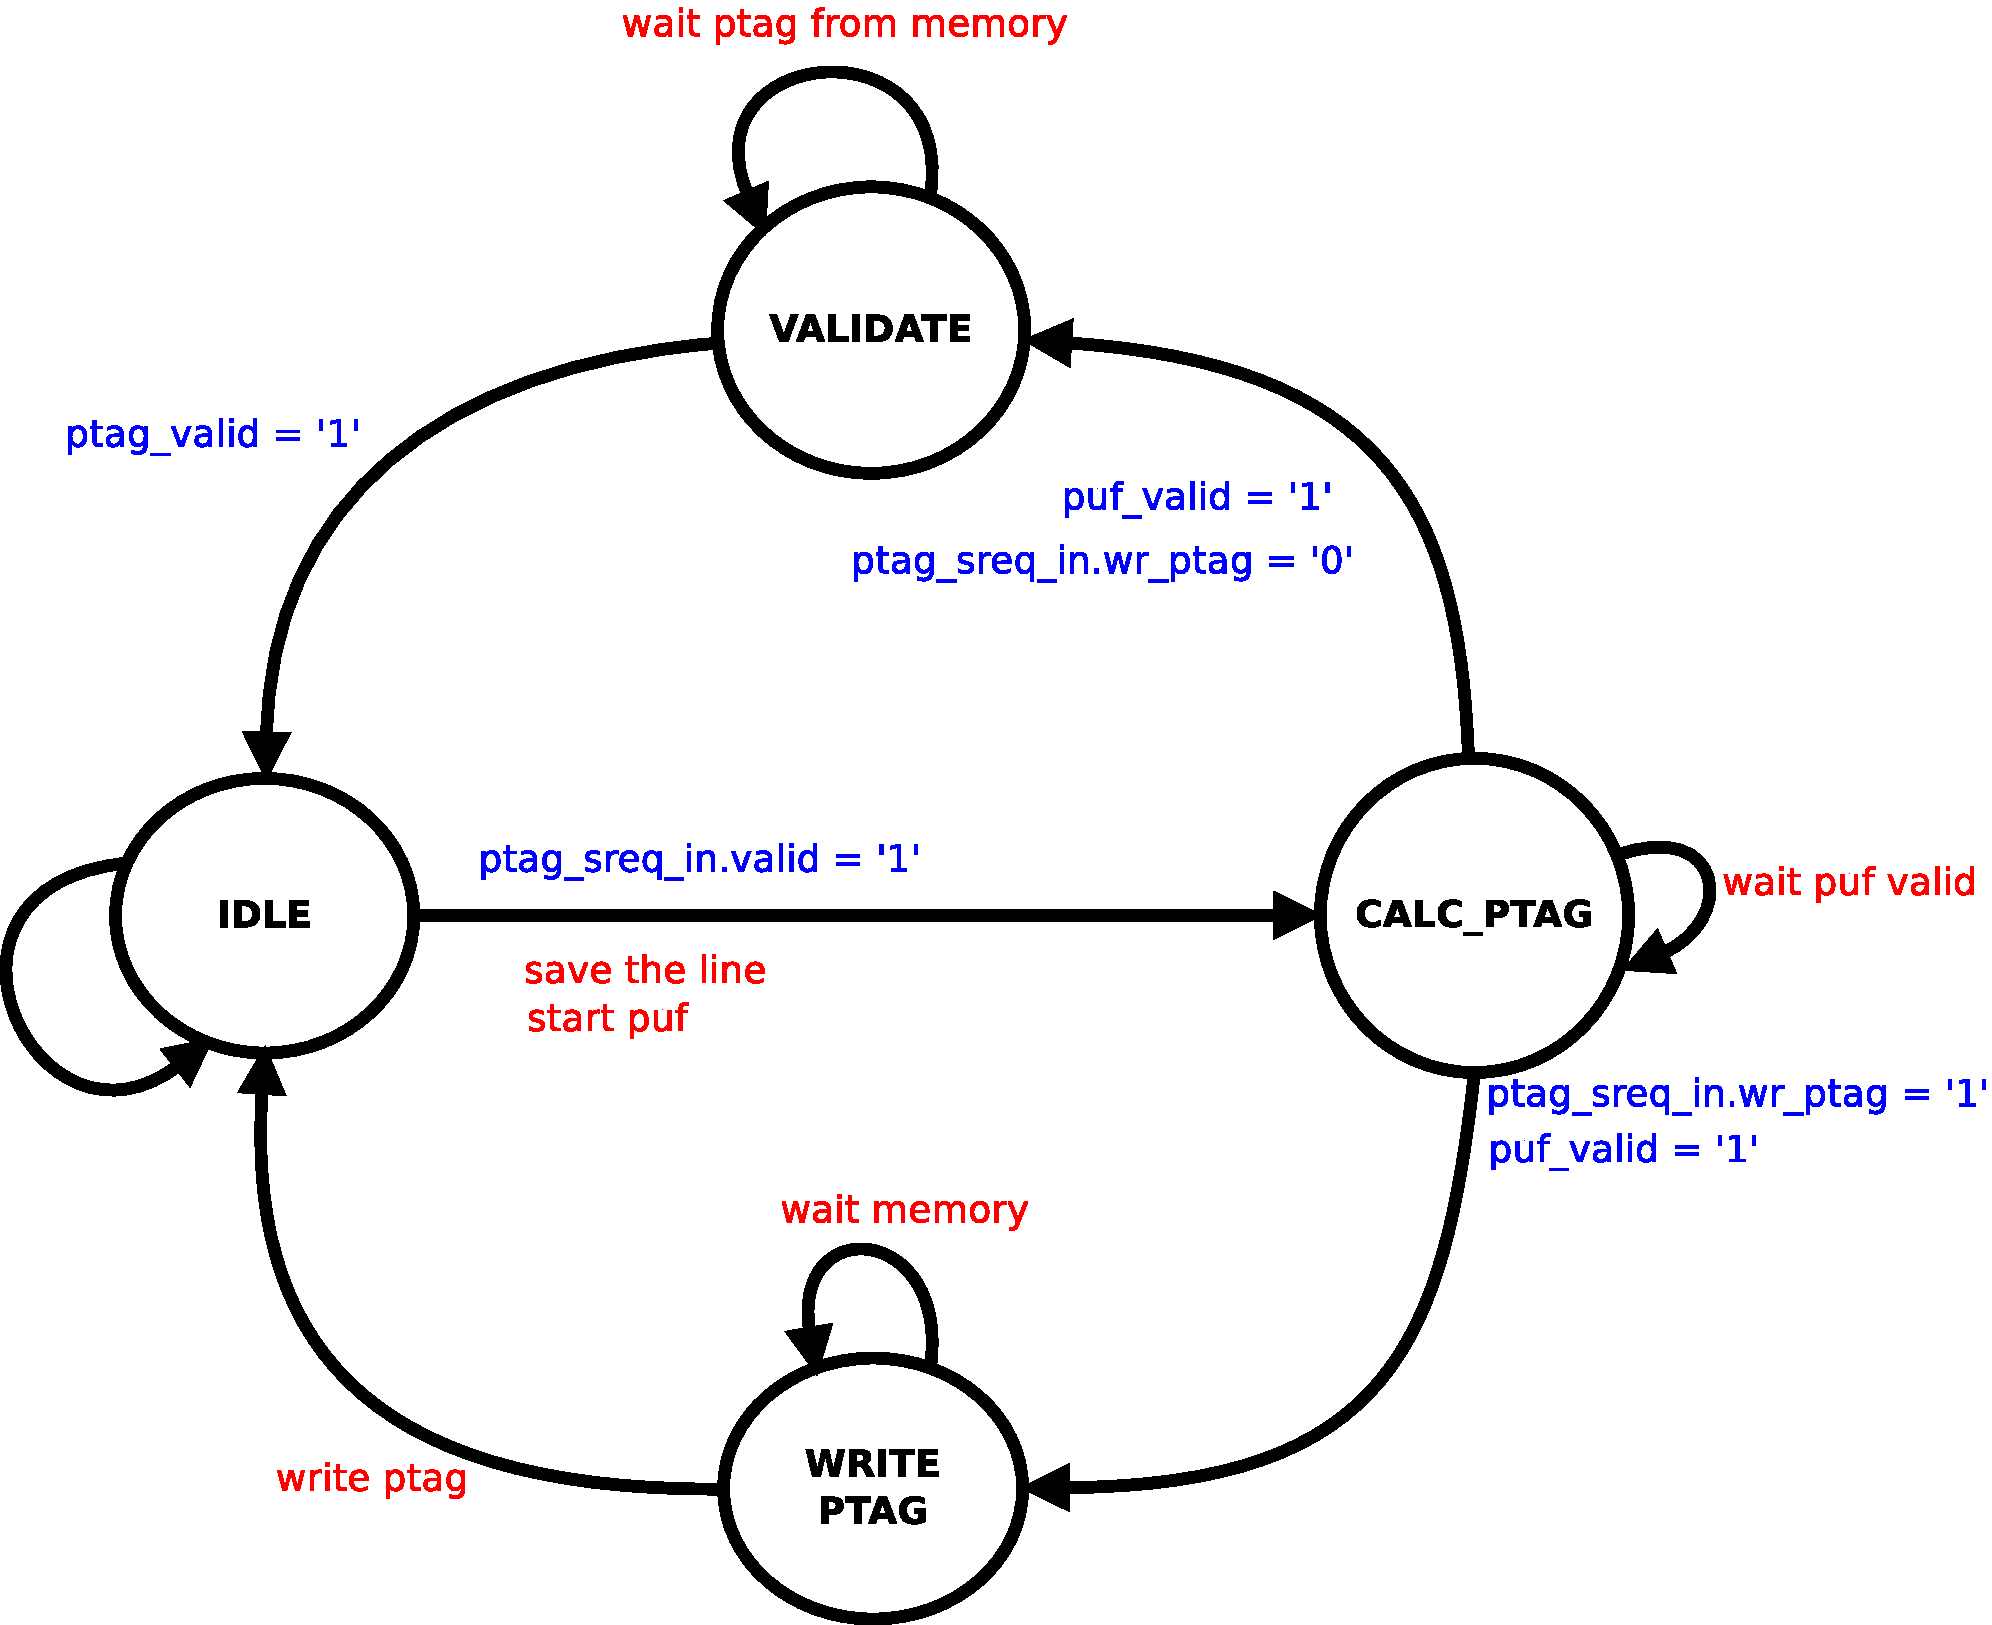
\includegraphics[width=0.70\textwidth]{figures/pdf/sec_engine_sm_no_tree.pdf}
    \caption{\seceng~ state  machine. }
    \label{fig:sesm}
\end{figure}

The \seceng~ is the core of \cshia~, here all the security features take place. This block has the following features: 
\begin{enumerate}
    \item Extract the cryptographic key from the SPUF
    \item Create the \ptags~for each \sline
    \item Validate \ptags an inform the \handler~that the execution is secure
    \item Control the \ptagmem~ 
\end{enumerate}
%TODO remove the tree from the thesis
%There are two possible configurations for the \seceng~, with or without a \mt~ to provide integrity, both options are evaluated in Section \ref{sec:hardware_setup}.
 The implementation of \seceng~ uses a state machine illustrated in Figure \ref{fig:sesm} to synchronize the internal components. The state machine transactions will be used to explain how \seceng~ works.


\begin{itemize}
  \item{\textbf{IDLE}}
 
The \seceng ~ stays in the IDLE  state until a valid \sline~ is sent by the \handler~ when the line arrives either is to write or validate a \ptag~, for both cases, the line will be registered and a \ptag~will be generated, so the next state will be CALC PTAG. 
 
  \item{\textbf{CALC PTAG}}
  After a \sline~ is registered in IDLE state it is used to generate a \ptag, a process that can take many clock cycles. After the \ptag is ready, the initial controls signal from the \handler~ are evaluated and the state is set to either VALIDATE or  WRITE PTAG if this is a write operation. If the next state is  VALIDATE, a request is made to the \pmmu~ to fetch the previously calculated \ptag ~ of the equivalent \sline.
  

  \item{\textbf{VALIDATE}}
  Since in this state the \ptag~ from the \ptagmem and the newly generated one from the CALC PTAG state are ready, the comparison between the two values can be done and the result as a security response to the \handler~ can be sent. Then the system goes back to IDLE.
  

 \item{\textbf{WRITE PTAG}}
  This state signalizes to the \pmmu~  that the \ptag~ from the CALC PTAG state can be written in the \ptagmem~ and confirmation to the \handler~ is sent.
\end{itemize}


\subsubsection{\seceng~ operation }
The\seceng~ operations described in the previous sections can be better visualized as a continuous operation, for this the validate and the write transactions are described next.
\begin{itemize}
 \item{\textbf{Validate \ptag~ - }} As can be seen in Figure \ref{fig:ptgag_rd_no_mt}  on time $2$ the \handler~ sends a  \sline to the \seceng~, the line is registered and the generation of the \ptag~ starts, when the ptag\_ready signal is asserted,  the equivalent \ptag~ for the \sline~ is requested from the \ptagmem~. On time $4$ in one cycle the comparison is made and if the \ptags~ match a line\_secure flag is asserted and the \handler can continue to serve the processor.
 
   \begin{figure}[!ht]
    \centering
    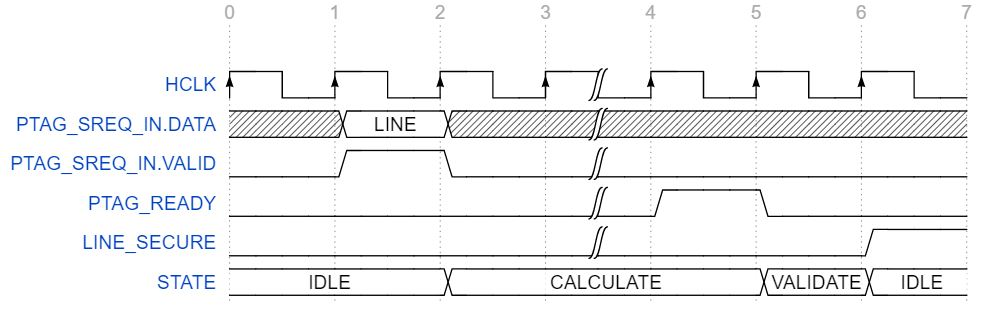
\includegraphics[width=\textwidth]{figures/others/ptag_read_sec_eng.JPG}
    \caption{\ptag~ read and validate on \seceng.}
    \label{fig:ptgag_rd_no_mt}
\end{figure}


 \item{\textbf{Write \ptag~ - }} for a write operation, like in the example from  Figure \ref{fig:ptgag_rd_no_mt}, the \sline~ that  come from \handler~  on time $2$ together with a write request are registered on IDLE state.  Next a new \ptag~ is generated in the CALC PTAG state, after the \ptag~is ready and the ptag\_ready signal is asserted on time $5$, a request to the \pmmu~ is made  to write the new \ptag in the \ptagmem on time $6$, finally the state is back to IDLE  and a line\_secure flag is asserted on time $9$ so the \handler~ can continue its operation. 
   \begin{figure}[!ht]
    \centering
    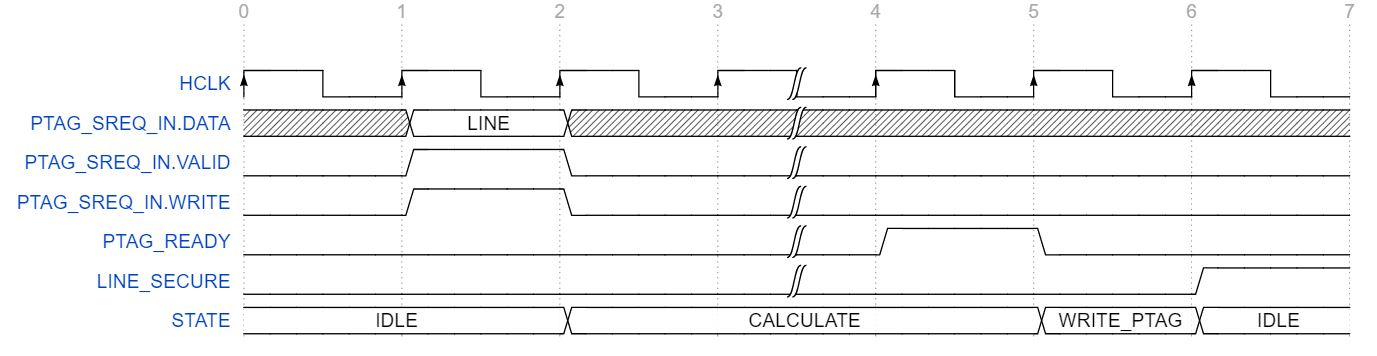
\includegraphics[width=\textwidth]{figures/others/ptag_write_sec_eng.JPG}
    \caption{\ptag~ write  on \seceng.}
    \label{fig:se_pw_no_mt}
\end{figure}
\end{itemize}

%  \begin{figure}[H]
%    \centering
%    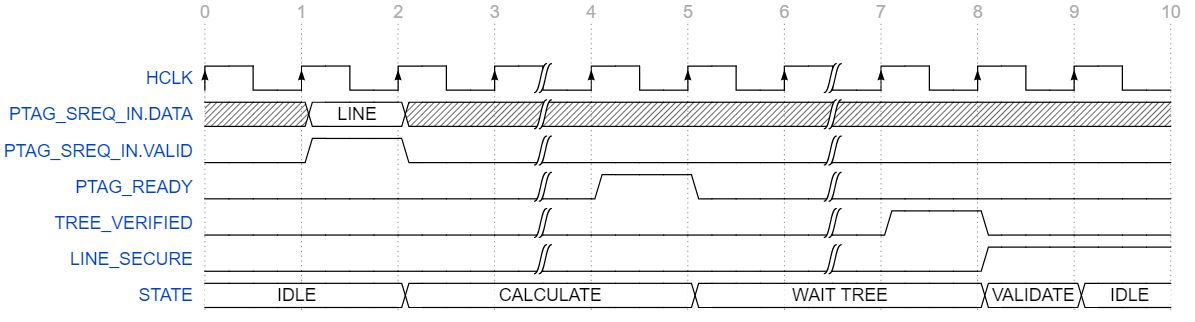
\includegraphics[width=\textwidth]{figures/ptag_read_tree_sec_eng.JPG}
%    \caption{\ptag~ read with \mt }
%    \label{fig:ptgag_rd_mt}
%\end{figure}
%  \begin{figure}[H]
%    \centering
%    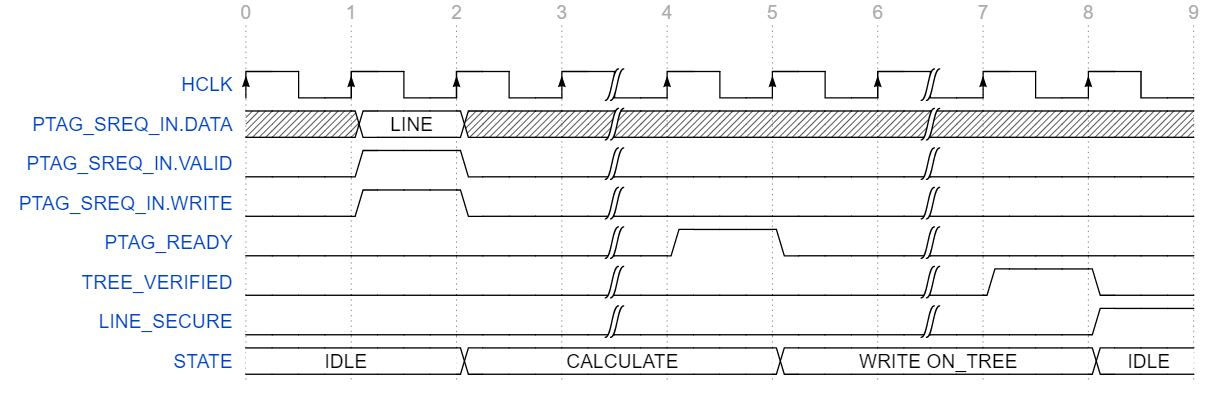
\includegraphics[width=\textwidth]{figures/ptag_write_tree_sec_eng.JPG}
%    \caption{\ptag~ write  on sec engine with \mt.  }
%    \label{fig:se_pw_mt}
%\end{figure}
%===========================================================================================================================================================




\subsection{\ptag~ Memory Management Unit (\pmmu)}
\label{subsec:pmmu}
The main functions of the \pmmu~are to store and request \ptags~from the \ptagmem~ and also to decode internal addresses of \ptags~to physical addresses of \ptagmem. This block is required every time the \handler~ needs to execute a security check, it needs to provide the \ptag ~ from the equivalent \slines~  to be compared in the VALIDATE state of the \seceng~  and write the newly generated \ptags when requested in the WRITE PTAG state of the \seceng.  Other blocks of \cshia~ are agnostic to the \pmmu operation since it controls the \ptagmem~ that is not connected to the bus.
 %In addition to that, \pmmu~can have two distinct designs. 
%If a designer chooses to use timestamps as the solution for replay attacks, \pmmu~will have an internal memory to store and control timestamps of the memory blocks.
% However, if the solution for replay attacks is a \mt\cite{Elbaz2009}, \pmmu~will control verification and update of the tree, as well as it will have cache memory, the \ptagcache, to speed up these tasks.
%\subsubsection{\ptagmem}
%\label{subsubsec:ptagmem}
%\augusto{describe memories connected to  PMMU}


\section{Operation Modes}
\label{sec:opmodes}

%describe all


\subsection{Runtime Phase}
\label{subsec:runtimephase}
\def\fenroll{Figure \ref{fig:fuzzy-extractor} \subref{fig:fuzzy-enroll}}
\def\fregen{Figure \ref{fig:fuzzy-extractor} \subref{fig:fuzzy-regen}}
After the enrollment phase, \cshia~instances are ready for distribution. Here is how \cshia's components work together. \handler~checks for memory read-write operations of the processor. When it perceives a memory read, it will capture memory words \andor~request memory words to compose a memory block. Then it sends this memory block and its address to \seceng. On its turn, \seceng~uses \pmmu~to bring the corresponding \ptag~of that memory block from \ptagmem, while \ptaggen~computes a \ptag~using the content served by \handler. After that, the \ptag~brought from \ptagmem~and the one computed are compared. If they match, \seceng~knows that neither the \ptag~nor the memory block were tampered with. Otherwise, \seceng~alerts the handler that can isolate the processor or sends a non-maskable interrupt to the processor.


For write operations, the process is more straightforward. Once any memory block that reached the processor was verified for integrity and authenticity, \handler~can serve the cache line to \seceng~that uses \ptaggen~to compute a new \ptag~and \pmmu~sends that \ptag~to \ptagmem.  During the product lifetime, the device can be rebooted and turned off and on multiple times. While this will not affect \ptags, which are externally stored in \ptagmem, the secret key has to be recovered every time the system comes back from off-line periods. This recovery procedure of the \fuzzy~is described next.

\subsubsection{Key Regeneration}
\label{subsubsec:Key-Regenation}
\begin{figure}[!t]
    \centering
    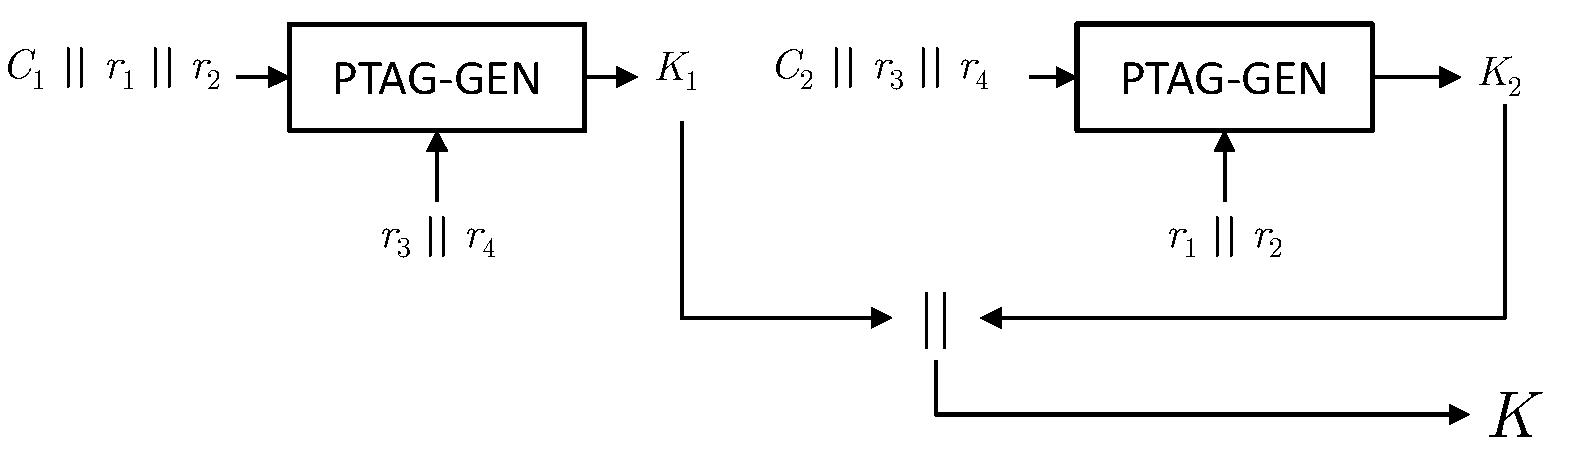
\includegraphics[width=0.7\textwidth]{key-construction}
%     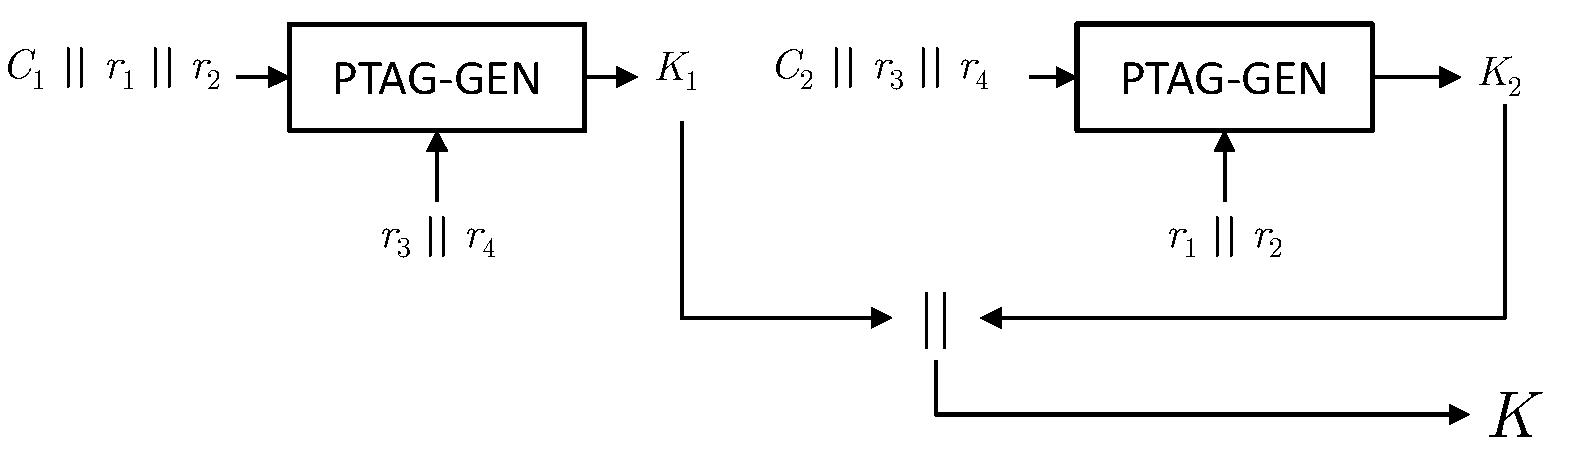
\includegraphics[scale=0.325]{key-construction}
    \caption{Key generation on \cshia.}
    \label{fig:key-construction}
\end{figure}

During the enrollment, there were eight challenges selected to produce four $r_i$ and four $w_i$ values. These challenges and helper data can be exposed off-chip and stored in \ptag~Memory if the designer chooses to do so. The recovery process of the secret key can be seen in \fregen. After using the challenges and all helper data, the syndromes are recovered. Due to inconsistent nature of \pufs, the fuzzy extractor actually recovers bit-flipped versions $w'_i$ and $r'_i$, what leads to the \bch~decoder receive $r'$ and $s'$. Once bit flips in $r_i$ values are corrected, the \fe~uses all $r_i$ to regenerate the secret key as Figure \ref{fig:key-construction} shows.

\subsection{Enrollment Phase}
\label{subsec:Enrollment-Phase}

In order to ensure authenticity and integrity, an initial procedure has to be conducted by the manufacturer\slash{}vendor. This enrollment procedure will activate the \fuzzy~to to extract the secret key from \pufs. Once that is done, the \handler~brings all memory blocks for tag generation. Next, this procedure is explained in detail.

\subsubsection{Key Extraction}
\label{subsubsec:Key-Extraction}

\ptag~Generator implements a Pseudo-Random Function (\prf), which is a primitive cryptographic very similar to a hash function with a significant difference: the input processing is based on a secret key. In order to provide uniqueness to every \cshia~ instance this key has to be unique. As aforementioned, \pufs~cannot be cloned, thus they can provide this uniqueness. Nevertheless, one big conundrum of using electronic \pufs~to generate keys is that they are inherently unstable. Due to their nature of leveraging on the imperfection of the fabrication process, external factors such as temperature variation, voltage variation, etc., can interfere with their responses. Thus, varying responses to challenges during the lifetime of devices. In order to provide consistency in \puf~responses, \fuzzy~(\fe) are employed. In simple terms, \fes~are schemes comprised of an extraction algorithm and a recovery procedure. Becker provides a solid review and formal definitions in \cite{Becker2017:RobustFuzzyExtractor}.

There are multiple ways of implementing a \fuzzy. Originally, \cshia~was proposed using a Code-offset \fe, which is well-known to reduce the entropy of extracted keys \cite{Armknecht2011:Formalization}. To strengthen the \cshia~design, we now use an adapted version of the Index-based Syndrome (\ibs) \fe~proposed by Yu and Devadas in \cite{Yu2010:RobustErrorCorrection}. \fenroll~illustrates the process of key extraction of \cshia's \fe. In general terms, a bit string $r$ is extracted from \pufs. Then, the \fe~generates a syndrome $s$ of $r$ using a $(n,k,t)$ Error Correction Code (\ecc). The \fe~also extracts a bit string $w$ and combines it to the syndrome $s$ to generate an encoded helper data $h$. This helper data $h$ can be externally exposed and will not leak information about $r$ (that can be used as a secret key or derive the key).


\begin{figure}
     \centering
     \begin{subfigure}[b]{0.5\textwidth}
         \centering
         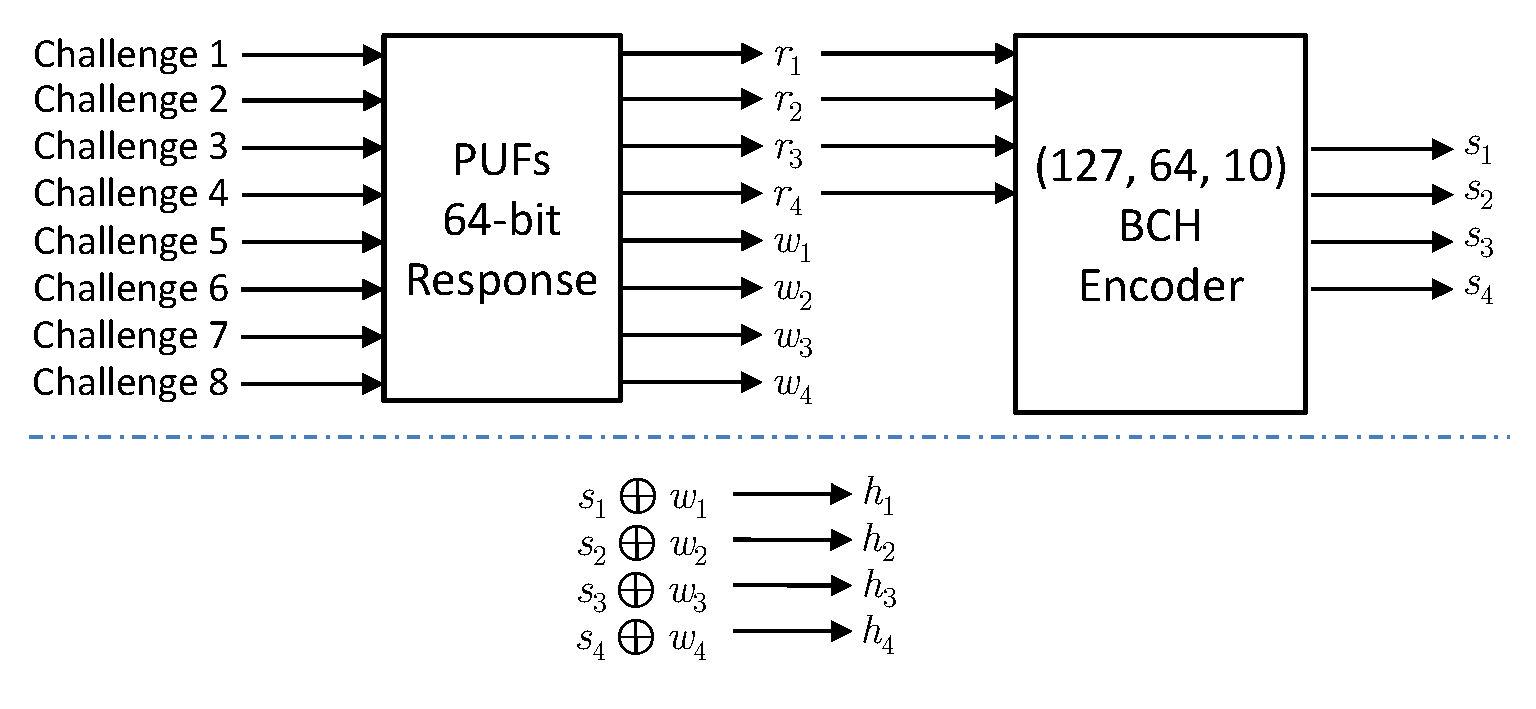
\includegraphics[width=\textwidth]{fuzzy-enroll}
         \caption{\fuzzy~during key extraction.}
         \label{fig:fuzzy-enroll}
     \end{subfigure}
     \hfill
     \begin{subfigure}[b]{0.5\textwidth}
         \centering
         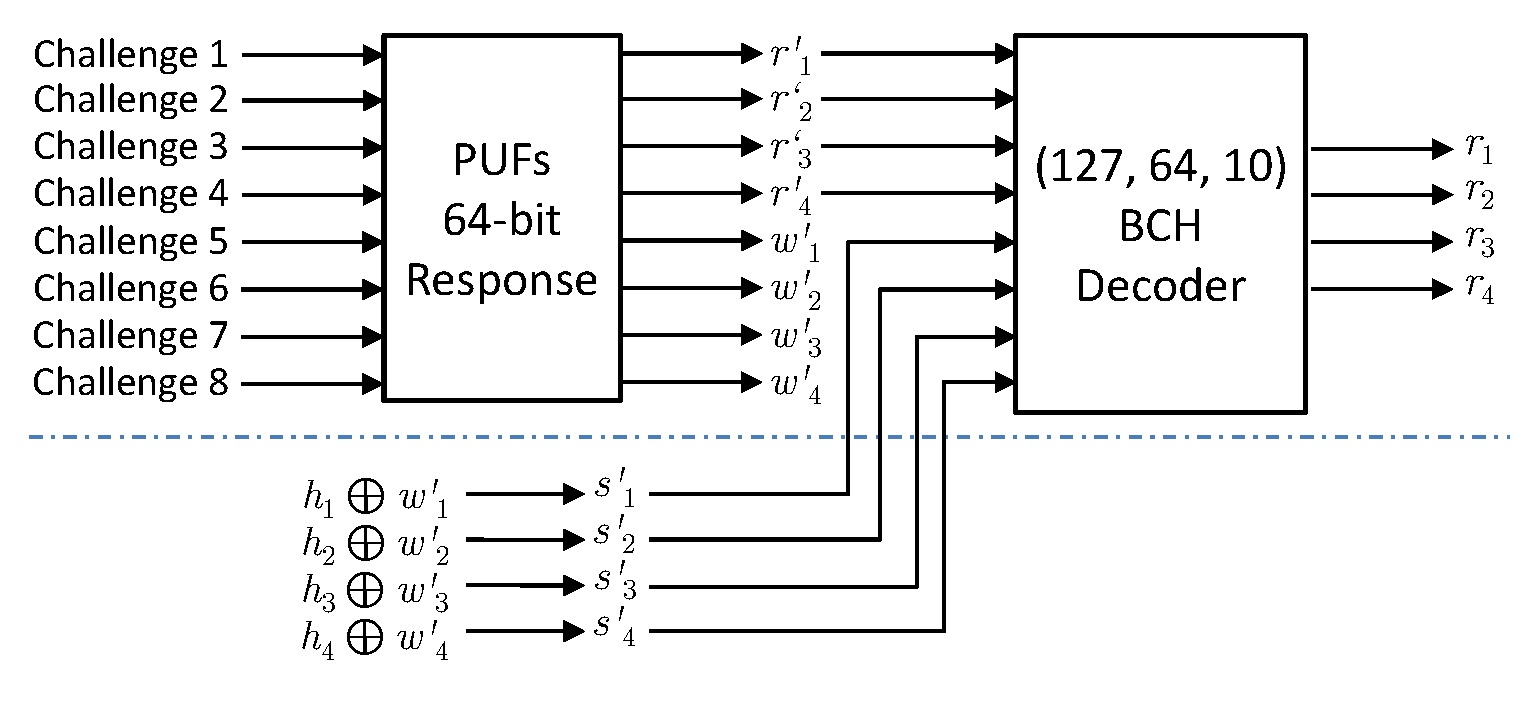
\includegraphics[width=\textwidth]{fuzzy-regen}
         \caption{\fuzzy~during key regeneration.}
         \label{fig:fuzzy-regen}
     \end{subfigure}

        \caption{\fuzzy~actions during the enrollment and recovery procedure.}
        \label{fig:fuzzy-extractor}
\end{figure}

To fully explain \fenroll, the chosen parameters are detailed. First, \cshia~incorporates \pufs~that produce 64-bit responses. These \pufs~ will be responsible for generating each string $r$ and $w$ that are 64 bits long. To match the length of $r$ and $w$, \cshia~has a $(127, 64, 10)$-\bch~\ecc. As \fenroll~depicts, there are four-bit strings $r_i$, which are compounded two by two and fed to the \prf~(Figure \ref{fig:key-construction}). Such combinations were specifically designed to match the \prf~chosen for \cshia, the \siphash~\cite{Aumasson2012:SipHash}, which has an output of 64 bits and uses a key of 128 bits. Therefore, the first pair of bit strings $r_i$ is concatenated with a constant and processed by the \prf~using the second pair of bit string $r_i$ as key. That generates a hash $K_1$. Then, inverting their places and concatenating the second pair with a different constant, a hash $K_2$ is obtained. Concatenating $K_1$ with $K_2$ results in $K$ which is the secret key of \cshia. Notice that $C_1$ and $C_2$ in Figure \ref{fig:key-construction} are replacing addresses for input of the \ptaggen. One can notice that assuming that each bit string $r_i$ has at least half of their length of entropy, each part of the key will have full entropy. Hence, the key has full entropy. 

\subsubsection{Full Memory Protection}
\label{subsubsec:Full-Memory-Protection}

The Enrollment Phase proceeds to tag the memory range the manufacturer\slash{}vendor specified during design. Now that \ptaggen~has a unique key, \seceng~orders \handler~to bring all memory blocks and deliver them to it. \seceng~will use \ptaggen~to generate \ptags.%, however, depending on the solution against replay attacks a designer chooses, \ptaggen~is used differently. 

% \paragraph{Timestamps Generation}
% \label{paragraph:Timestamps-Generation}

% When timestamps are the solution against replay attacks, \pmmu~will have a timestamp memory. This timestamp memory has the depth of the number of data memory blocks the designer chose to cover. Thus, before \handler~hands in data memory blocks, \pmmu~will clear the entire timestamp memory to avoid uninitialized values. While \seceng~receives code memory blocks, generated \ptags~are just passed to \pmmu~that stores them in \ptagmem. As \handler~starts to pass data memory blocks to \seceng, \pmmu~increments the timestamp of each memory block received and passes this value to \seceng, which combines with the address of the memory block. This combination is then concatenated with the memory block and then finally hashed into a \ptag. \pmmu~receives this \ptag~and stores it in \ptagmem.

% \paragraph{\mt~Generation}
% \label{paragraph:Merkle-Tree-Generation}

% A \mt~solution is more complex. The first procedure is very straightforward. \seceng~receives memory blocks and their addresses from \handler~and uses \ptaggen~to generate \ptags. \pmmu~receives these \ptags~and sends them to \ptagmem. After all memory blocks had their \ptags~generated, \pmmu~starts to bring \ptags~of data memory blocks. As soon as a chunk of \ptags~is formed, a \ptag~internal address of the chunk is calculated. \pmmu~provides this internal address and the chunk to \ptaggen~that generates a \ptag. This \ptag~is returned to \pmmu~that stores it in \ptagmem. This process will continuously happen (as we can see in Figure \ref{fig:vtree}) until \pmmu~identify that the last \ptag~calculated has no siblings. Hence, it is the root \ptag, which must be stored inside \pmmu. It is worth to clarify that \ptag~internal address is an address space that facilitates computation and identification of descendants and ancestors. Each internal address is directly translated to a physical address by \pmmu~and this translation has as goal to minimize unused spaces in \ptagmem. Moreover, in terms of security, this internal address mitigates a very specific attack on the tree, in which an descendant has the same \ptag~as one of its ancestors. In this case, an attacker could try to perform a relocation attack likewise. 


\chapter{CSHIA  Prototype}
\label{chap:cshia_prototype}


%   \section{Security Analysis} \label{sec:security}
   \begin{figure*}[!htb]
	  \centering
	  \includegraphics[scale=0.2]{sec_engine_tetec}
	  \caption{The prototype architecture.}
  %	\vspace*{-9pt} 
	  \label{fig:protcshia}
  \end{figure*}

   The prototype will be implemented upon a Leon 3 SPARC V8 platform from Aeroflex Gaisler~\cite{Leon} on an Altera DE2-115 Development Kit. To implement \cshia's pre design (Figure \ref{fig:system}), the design of two blocks are planned: the Security Engine (\tagsystem) and the Security Cache (\seccache) , to be inserted between the processor and the memory controller as shown in Figure \ref{fig:protcshia}. The \seccache~ will control bus transactions between the processor and the \mctrl, and provide data to the \tagsystem. Consequently, the \tagsystem~ will control the fuzzy extractor and the \ptaggen. To use  \cshia's fuzzy extractor a (127, 64, 10)-\bch~code instance for error correction and  an internal memory that emulates a \spuf will be used. The \ptaggen~ will use a \siphash-2-4 for \ptag~generation and verification.



  \subsection{Prototype Configuration}
  \label{subsec:cshia-configuration}

  
  Since the processor may ask for an arbitrary number of words from memory, and the architecture needs to check for the integrity of a full memory block in every cache miss, a buffer in \seccache will be used to hold isolated memory words required by the processor. When the processor demands a memory word, the buffer controller will request all the other words from the main memory to fit one \ptag block. That will allow \cshia~to authenticate entire memory blocks and,with the proper memory size, can also speedup sequential requests of the processor. The buffer will be configurable to fit a variable \ptag~block. 
  %for this work it is implemented in two separate blocks, one for reads and another one for writes, with only 256 bytes each. Because the current \cshia~prototype was planned as a preliminary platform for security evaluation, there are many auxiliary components and additional memories not present in the original Leon 3 platform. 
 
 


\chapter{CSHIA  Evaluation}
\label{chap:cshia:evaluation}


This chapter describes the experimental setup and results. First, it describes benchmarks and experiments configuration. Then, it presents experimental results on performance, area and power estimates.
\augusto{removed the Merkle tree tradeoff and analysis}


\section{Experimental Setup}
\label{subsec:Experimental-Setup}

Using \grmon, we are able to load programs, measure runtime, insert breakpoints, and set some \leon~parameters. As benchmarks, we chose nine programs from the MiBench suite \cite{MiBench}: \texttt{basicmath}; \texttt{bitcount}; \texttt{susan}; \texttt{qsort}; \texttt{fft}; \texttt{fft\_inv}; \texttt{sha}; \texttt{stringsearch} (or just \texttt{search} for short). These benchmarks were either executable without input files or easily modified to run without them. Thus, for some benchmarks we incorporated input files in their data segment, and these modifications were evaluated against reference outputs. MiBench usually provides two types of inputs: small and large. We ran both inputs for most of the benchmarks, except by \texttt{basicmath}, \texttt{fft}, and \texttt{fft\_inv}. The large inputs of these programs did not affect the size of the data segment and yet most of their run time was dominated by printing their outputs over \grmon.

As Section \ref{sec:hardware_setup} discussed, the \cshia~implementation is able to cover up to 512 KB of data. This was enough for most of the benchmarks except by the large inputs of \texttt{qsort} and \texttt{sha}, as Table \ref{tab:benchmarks} shows. Only the \texttt{.data} and \texttt{.bss} segments of the programs were covered. We did not have enough memory to reach the beginning of the \texttt{.stack} segment and we would only were able to cover a small portion of \texttt{.heap} segment.

Each benchmark was run in eight different instances of \cshia in \cite{caio}\augusto{i have to find out how to include caios work}. (1) The first \cshia~instance is the one that \handler~is disabled and bypasses incoming and outgoing bus transfers from the processor. We called this instance as \baseline. (2) The second instance of \cshia~uses the timestamps solution against replay attacks. We defined it as \timestamp. (3-8) The remaining instances are variations of \cshia~when a \mt~is used as a solution against replay attacks. Since this works only evaluate the \cshia~ implementation and not the tradeoffs of the \cshia~ extended security features, we will compare the (1) and (2) with (3) \cshiamt-64x2-\lru , an instance of \cshia~ with a \mt~ and \ptagcache of $64$ lines and $2$ sets.

\begin{table}[t]
	\center
	\caption{Coverage of data segment in benchmarks.}
	\label{tab:benchmarks}
	\footnotesize
	\begin{tabular}{|l|c|c|}
%\		\noalign{\hrule height 1pt}
%\		\rowcolor{lightgray}
		\hline
			Benchmark & .data segment size (KB) & Cover (\%)\\ 
		%\noalign{\hrule height 0.75pt}
		\hline
		\hline
			\texttt{qsort\_small}		&	54.9	&	100		\\
			\texttt{qsort\_large}		&	588.6	&	86.99	\\
			\texttt{bitcount\_small}	&	3.3		&	100		\\
			\texttt{bitcount\_large}	&	3.3		&	100		\\
			\texttt{sha\_small}			&	307.2	&	100		\\
			\texttt{sha\_large}			&	3174.4	&	16.13	\\
			\texttt{search\_small}		&	3.4		&	100		\\
			\texttt{search\_large}		&	13.4	&	100		\\
			\texttt{fft\_small}			&	2.7		&	100		\\
			\texttt{fft\_small\_inv}	&	2.7		&	100		\\
			\texttt{dijkstra\_small}	&	31.1	&	100		\\
			\texttt{dijkstra\_large}	&	31.1	&	100		\\
			\texttt{basicmath\_small}	&	2.7		&	100		\\
			\texttt{susan\_small}		&	23.9	&	100		\\
			\texttt{susan\_large}		&	326.7	&	100		\\
		\hline
	\end{tabular}
%\vspace*{-12pt}
\end{table}

\section{Performance Analysis}
\label{subsec:Performance-Analysis}

%\begin{figure}[!t]
%	\centering
%	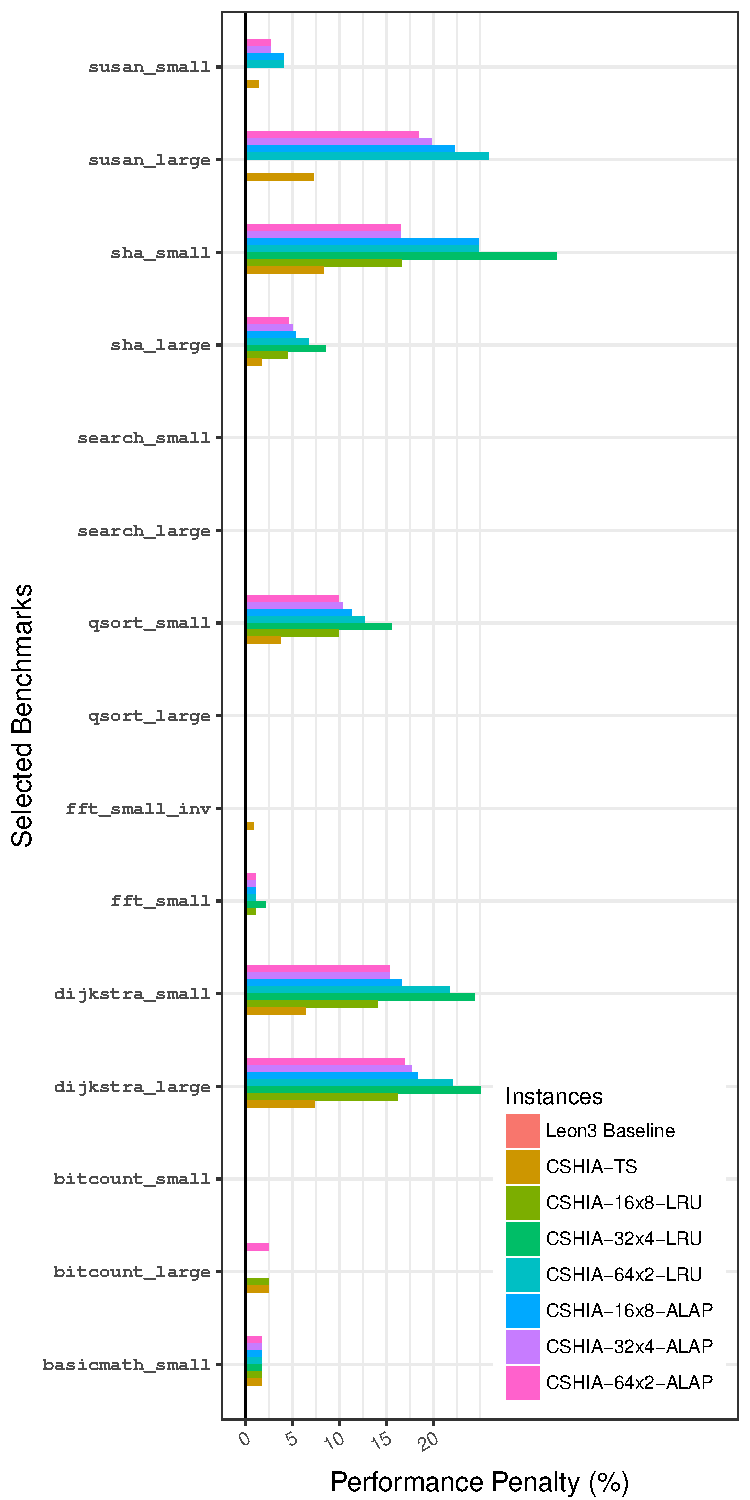
\includegraphics[scale=0.7]{benchmarks.pdf}
%	\caption{Execution time for benchmarks. For each benchmark, the running time was normalized by Leon's running time.}
%	\vspace*{-9pt} 
%	\label{fig:benchmarks}
%\end{figure}

\begin{table*}[t]
	\center
	\caption{Performance overhead in \% of the evaluated \cshia~instances in comparison of running times in \baseline.}
	\label{tab:results}
	\footnotesize
	\begin{tabular}{|l|c|c|}
%\		\noalign{\hrule height 1pt}
%\		\rowcolor{lightgray}
		\hline

	    Benchmarks				& \timestamp (\%)	& \cshiamt~instance(64x2-\lru)(\%)\\

		\hline
		\hline
		\texttt{qsort\_small}				& 	3.77	&	9.90\\
		\texttt{qsort\_large}				& 	0.05	&	0.05\\
		\texttt{bitcount\_small}			& 	0.00	&	0.00\\
		\texttt{bitcount\_large}			& 	2.43	&	0.00\\
		\texttt{sha\_small}					& 	8.31	&	16.55\\
		\texttt{sha\_large}					& 	1.78	&	4.75\\
		\texttt{search\_small}				& 	0.10	&	0.00\\
		\texttt{search\_large}				& 	0.00	&	0.01\\
		\texttt{fft\_small}					& 	0.00	&	1.07\\
		\texttt{fft\_small\_inv}			& 	0.92	&	0.00\\
		\texttt{dijkstra\_small}			& 	6.40	&	14.09\\
		\texttt{dijkstra\_large}			& 	7.35	&	16.90\\
		\texttt{basicmath\_small}			& 	1.73	&	1.73\\
		\texttt{susan\_small}				& 	1.37	&	2.73\\
		\texttt{susan\_large}				& 	7.23	&	18.72\\
		\hline
		\textit{\textbf{Average}}			&	\textbf{2.76}	&	\textbf{5.77}\\

		\hline
	\end{tabular}
%\vspace*{-12pt}
\end{table*}

Table \ref{tab:results} shows our results. The first conclusion is that \timestamp~performs better than the instance using the \mt. \timestamp~worst performance penalty is 8.30 \% for \texttt{sha\_small} and has an average performance penalty of just 2.76 \%. Because \cshia~could not entirely cover \texttt{sha\_large}, its performance penalty ended up being smaller than its counterpart. The \texttt{bitcount} and \texttt{fft} benchmarks had inconsistent results in some cases, when comparing all instances together. Delving into reasons for that, we found out that they are dependent of random number generation and this was affected by the intervention of \cshia~in the \amba~bus. Therefore, for those benchmarks, the performance difference between \cshia~instances should not be considered significant. Another observation regards to \texttt{qsort\_small} and \texttt{qsort\_large}. They presented similar behavior of the \texttt{sha}~benchmarks, despite \cshia~almost entirely covers the data segment of \texttt{qsort\_large}. 

Because verification of \ptags~of code memory blocks is equal in \timestamp~and \cshiamt, the only way to improve performance of \cshia~is reducing the number of accesses to \ptagmem~for data memory blocks. Thus, increasing the \ptag~cache size may lead \cshiamt~to obtain better performance than \timestamp. Obviously, these choices need to take into account other variables such as area and power, which we discuss next.

\section{Area and Power Estimates}
\label{subsec:Power-and-Area-Estimative}

Since we did not have access to standard tools from industry to synthesize \vhdl, we used the area and power proportionality relation \cite{Nemani1999:Area-Power} to compute our estimations. For that, we used well-known open tools like \cacti~5.3 \cite{HP:Cacti53} for cache memories estimative of power and area, and Ahmed \etal's work~\cite{Ahmed2009:Leon} that presents area and power for a synthesized \leon~processor on 65 nm LPLVT (Low Power Low Voltage Threshold) process using ST Microelectronics libraries.

Ahmed \etal~presented their \leon~design separating area, static and dynamic power for the core and its cache memory. We ignore their cache memory values since they differ from our implementation. Moreover, our primary goal is to estimate the area of logic elements. Thus, we will assume a proportional relation between their core area, 0.191 mm$^{2}$, and the number of \fpga~logic elements of the \baseline~implementation, which is 23,629 in the Altera's DE2-115 development kit. %tat static power (at 25\textordmasculine) 85.3 $\mu$W and dynamic power (at 100 MHz) was 5.75 mW. Although \cshia's~\fpga~implementation runs at 50 MHz, we can use Ahmed \etal~results to estimate \cshia's area overhead. As well as, for power, we can compute \leon's and \cshia's power using Intel's Early Power Estimators (\epe) \cite{Intel:EPE} for \fpgas~and deduce an estimative based on the ASIC power consumption of Ahmed \etal

Through this proportional relation between area and logic elements, our estimate for the \timestamp~and \cshiamt, without additional memories, is 0.246 mm$^{2}$ and 0.264 mm$^{2}$, respectively. As we said, area and power can be proportional, and thus we can use similar reasoning to estimate power. From Ahmed \etal's work, static and dynamic power (at 100 MHz) are 85.3 $\mu$W and 5.75 mW, respectively. Those numbers result in static power of 109.48 $\mu$W for \timestamp~and 117.41 $\mu$W for \cshiamt. In terms of dynamic power, we obtained 7.41 mW for \timestamp~and 7.94 mW for \cshiamt.
\begin{table}[!ht]
	\center
	\caption{Area and power for \cshia~implementation~without considering instruction and data cache memories of the processor.}
	\label{tab:area-power}
	\footnotesize
	\begin{tabular}{|l|l|p{0.65in}|p{0.6in}|}
%\		\noalign{\hrule height 1pt}
%\		\rowcolor{lightgray}
		\hline
			\multirow{2}{*}{Instance} & \multirow{2}{*}{Area (mm$^{2}$)} & Static & Dynamic\\ 
			 & & Power (mW) & Power (mW)\\ 
		%\noalign{\hrule height 0.75pt}
		\hline
		\hline
			\baseline & & & \\
				\hspace{0.25in} Core & 0.191 & 85.3 $\times~10^{-3}$ & 5.75 \\
			\timestamp & & & \\
				\hspace{0.25in} Core & 0.246 & 109.48 $\times~10^{-3}$ & 7.41 \\
				\hspace{0.25in} Memory & 0.141 & 72.00 & 7.15  \\
				\hspace{0.25in} \textbf{Total} & 0.387 & 72.11 & 14.56  \\
			\cshiamt-64x2 & & & \\
				\hspace{0.25in} Core & 0.264 & 117.41 $\times~10^{-3}$ & 7.94 \\
				\hspace{0.25in} Cache & 0.274 & 6.90 & 100.98  \\
				\hspace{0.25in} \textbf{Total} & 0.538 & 7.02 & 108.92 \\
		\hline
	\end{tabular}
%\vspace*{-12pt}
\end{table}

We used \cacti~to estimate how the timestamp memory and \ptagcache~affects the design. From Table \ref{tab:config}, the total timestamp memory size was 2 bytes $\times~2^{14}$ (or 32 KB). Even though \cacti~does do not offer an option for non-volatile estimative, a DRAM like estimation provides an insight of area and power. For the \ptagcache, we estimated 4-KB \ptagcache~with 64 lines and two sets, all estimations are summarized in Table \ref{tab:area-power}. 



Even if our estimates are not very accurate, they allow to analyze which solution would provide the best trade-off among area, power, and performance penalties. Thus, based on our numbers, the \timestamp~would be the best solution. Of course, that would only apply to this specific memory size we evaluated. In the security side, 16-bit timestamps will not provide the same security as our \cshiamt~instances with \ptags~of 64 bits. In addition, if the coverage of the data segment needs to be increased, the timestamp memory can reach prohibitive configurations for power and area. In such a situation, \cshiamt~would be capable of offering this higher coverage without impacting in on-chip power and area. Nonetheless, higher penalties in performance would happen. 


\chapter{Conclusion and Future Work}
\label{chap:conclusion}
    \section{Conclusion}
    \label{sec:conclusion}
    
\section{Future Work}
    \label{sec:future_work}
%\endgroup
% As referências:
\bibliographystyle{plain}
\bibliography{aqueiroz_msc_dissertation}



% Os anexos, se houver, vêm depois das referências:
%\appendix
%\chapter{Illustrative example files}
\label{appendix:example_files}

This appendix contains the plain text files that correspond to the
application, cloud, virtual machine repository, and generated
schedule of the illustrative example presented in subsection
\ref{sec:illustrative_example}.

\section{Application}


    \begin{tabular}{l c c l}
        $n$ & : & 4 &\\
        $I$ & : & [ & (1) 1 3 3 1]\\

        $S$ & : & [ & (1) 2 1 2 1]\\
        $B$ & : & [ & (1 1) 0 2 2 0 \\
            &   &   & (2 1) 0 0 0 1 \\
            &   &   & (3 1) 0 0 0 1 \\
            &   &   & (4 1) 0 0 0 0\\
            &   & ] & \\
        $D$ & : & [ & (1 1) 0 1 1 0 \\
            &   &   & (2 1) 0 0 0 1 \\
            &   &   & (3 1) 0 0 0 1 \\
            &   &   & (4 1) 0 0 0 0\\
            &   & ] & \\
    \end{tabular}



\section{Grid/Private Cloud}
    \begin{tabular}{l c c l}
        $m$  & : & 4 & \\       
        $TI$ & : & [ & (1) 1.000000 1.000000 1.000000 1.000000]\\
        $C$  & : & [ & (1) 1 1 1 1]\\

        $TB$ & : & [ & (0 1) 0.000000 2.000000 2.000000 2.000000 \\
             &   &   & (1 1) 2.000000 0.000000 2.000000 2.000000\\
             &   &   & (2 1) 2.000000 2.000000 0.000000 2.000000\\
             &   &   & (3 1) 2.000000 2.000000 2.000000 0.000000\\
             &   & ] & \\
        $N$  & : & [ & (0 1) 1 1 1 1\\
             &   &   & (1 1) 1 1 1 1\\
             &   &   & (2 1) 1 1 1 1\\
             &   &   & (3 1) 1 1 1 1\\
             &   & ] & \\
        $TR$ & : & [ & (1) 1.000000 1.000000 1.000000 1.000000]\\
    \end{tabular}



\section{Virtual machines repository}

    \begin{tabular}{l c c l}
        $o$  & : & 4 & \\
        $SV$ & : & [ & (1) 1 2 3 4]\\
        $BV$ & : & [ & (1) 4.000000 4.000000 4.000000 4.000000]\\
        $TV$ & : & [ & (1) 2.000000 2.000000 2.000000 2.000000]\\
    \end{tabular}



\section{Resulting schedule}

$T_{max}=24$
%     \chapter{The grid application generator}
    \ldots



\end{document}
